\documentclass[a4paper, 12pt]{book}

\RequirePackage[T1]{fontenc}
\usepackage{libertinus}

\usepackage{psl-cover}

\usepackage{subcaption}
\usepackage{graphicx} % Required for including images
\usepackage{tabularx}
\usepackage{footnote}
\usepackage[font=small,labelfont=bf]{caption} % Required for specifying captions to tables and figures
\usepackage{wrapfig} % Allows wrapping text around tables and figures
\usepackage{arydshln}
\usepackage{tikz}
\usepackage{pgfplots}
\usepackage{rotating}
\usepackage{flafter}

\usepackage{booktabs}
\usepackage{mathtools}
\usepackage{algorithm}
\usepackage{algorithmic}
\usepackage{gensymb}
\usepackage{epigraph}
\usepackage{csquotes}
\usepackage[toc,page]{appendix}
\usepackage{siunitx}
\usepackage{minted}
\setminted{fontsize=\footnotesize}
\setminted{breaklines}
\usepackage{etoolbox}
\AtBeginEnvironment{minted}{%
  \renewcommand{\fcolorbox}[4][]{#4}}
\usemintedstyle{bw}

\setmonofont{Inconsolata}
\usepackage{polyglossia}
\setdefaultlanguage{english}
\setotherlanguages{french,arabic}
\newfontfamily\arabicfont[Script=Arabic]{Amiri}

% nicer looking URLs
\usepackage{url}
\urlstyle{same}

\usepackage[style=ieee,backend=biber,maxnames=5]{biblatex}
\addbibresource{phd.bib}

\def\BibTeX{{\rm B\kern-.05em{\sc i\kern-.025em b}\kern-.08em
    T\kern-.1667em\lower.7ex\hbox{E}\kern-.125emX}}
\DeclarePairedDelimiter{\norm}{\vert}{\vert}

\makeatletter
\renewcommand\part{%
   \if@openright
     \cleardoublepage
   \else
     \clearpage
   \fi
   \thispagestyle{empty}%
   \if@twocolumn
     \onecolumn
     \@tempswatrue
   \else
     \@tempswafalse
   \fi
   \null\vfil
   \secdef\@part\@spart}
\makeatother

\usepackage{import}

\title{Improvements in Optical Character Recognition for Historical Arabic Manuscripts}

\author{Benjamin KIESSLING}

\institute{École Pratique des autes Études}
\doctoralschool{École doctorale de l'École Pratique des Hautes Études}{472}
\specialty{Voir spécialités ED}
\date{01 fevrier 2021}

%% cotutelle
%\entitle{Improvements in Optical Character Recognition for Historical Arabic Manuscripts}
%\otherinstitute{University of Leipzig}
%\logootherinstitute{logo-institute}

\jurymember{1}{Prénom NOM}{Titre, établissement}{Président}
\jurymember{2}{Prénom NOM}{Titre, établissement}{Rapporteur}
\jurymember{3}{Prénom NOM}{Titre, établissement}{Rapporteur}
\jurymember{4}{Prénom NOM}{Titre, établissement}{Examinateur}
\jurymember{5}{Prénom NOM}{Titre, établissement}{Examinateur}
\jurymember{6}{Prénom NOM}{Titre, établissement}{Examinateur}
\jurymember{7}{Prénom NOM}{Titre, établissement}{Examinateur}
\jurymember{8}{Marc BUI}{Directeur d'études, École Pratique des Hautes Études}{Directeur de thèse}
% \jurymember{9}{Prénom NOM}{Titre, établissement}{Invité}
% \jurymember{10}{Prénom NOM}{Titre, établissement}{Invité}

\frabstract{
	french abstract here
}

\enabstract{
	english abstract here
}

\frkeywords{ Caesar licentia post honoratis haec adhibens urbium
  honoratis nullum Caesar.}
\enkeywords{ Delatus delatus nominatus
  onere aut trahebatur quod tenus et bonorum.}

\begin{document}

\maketitle{}

\frontmatter
\input{layout/dedication.tex}
\cleardoublepage
\chapter*{Acknowledgements}
\thispagestyle{empty}

First, I would like to express my deepest gratitude to Marc Bui, who
accepted to supervise this thesis, for very interesting discussions, for his
valuable experience and guidance in matters both scientific and administrative.

I am so grateful to the eScripta team at EPHE and everyone at the Chair for
Digital Humanities at the University of Leipzig. Both provided an environment
were I was free to explore research ideas and their generous financial support
made my existence as a doctoral student a comfortable one. It was Maxim Romanov
through whom I had the first contact with Arabic text in Leipzig. I am also
eternally indebted to Daniel Stökl Ben Ezra and Peter Stokes for fending off
every imposition on my time during the last weeks of writing. 

I thank the OpenITI team for their incessant lobbying to get institutional
support for research into Arabic OCR. Without them, none of this would have
been possible. A special thanks goes to Matthew Thomas Miller and Jonathan
Allen who responded to my endless question on details of the Arabic script with
a celerity unheard of in academia.

The people of ALMAnaCH at INRIA should not be forgotten. They welcomed a
clueless foreigner on his arrival in France and integrated me in the lab.

I have wonderful friends who were there even at times when all they heard from
me was about this thesis. A huge thanks goes to Louise for helping improve the
French summary. Above all I thank Monika for reminding me in the darkest
moments that instant ramen is not the foundation of a balanced diet.

\cleardoublepage
\chapter{Résumé Long}

\begin{french}

\section{Introduction}

Cette thèse consiste en un certain nombre de publications qui étudient les
difficultés de la rétrodigitalisation de l'écriture arabe historique et propose
plusieurs méthodes pour faire progresser l'état de l'art en la matière. Bien
que ces méthodes visent principalement à remédier les problèmes résultant des
caractéristiques de l'écriture arabe, elles sont conçues pour être applicables
à l'écriture et aux inscriptions dans une variété d'autres systèmes d'écriture.

\section{L'analyse d'imges de documents et reconnaissance optique de caractères}

L'analyse d'images de documents (AID) est un sous-domaine de la vision par
ordinateur (VO) qui cherche à comprendre le contenu des documents par
le traitement de leurs images numériques.  Les documents sont définis
de façon libérale par le domaine, comprenant pas seulement les
documents manuscrits et le texte imprimé sur papier, mais aussi
l'écriture sur d'autres supports souples tels que le papyrus ou les
feuilles de palmier et même les inscriptions.

La différence vis-à-vis de la vision par ordinateur en général ne se trouve pas
dans les méthodes employées, mais dans la nature des images traitées.
Ces images sont généralement obtenues par des caméras ou des scanners,
souvent dans un contexte professionnel, ce qui permet d'obtenir un
matériel source avec un minimum de bruit provenant d'éléments non
pertinents que l'on rencontre souvent dans les images de scènes
naturelles traitées par d'autres branches du VO. Malgré des données d'entrée
plus propres, les représentations structurées souhaitées en sortie ont
tendance à être plus complexes et plus nombreuses dans la AID que dans
d'autres applications, nécessitant la détection, la classification et
la mise en relation de dizaines d'éléments de documents tels que des
lignes, des caractères, des illustrations et des tableaux.

Comme dans d'autres domaines de l'informatique, la recherche en DIA peut être
divisée en tâches spécifiques, dont une ou plusieurs sont résolues par
une méthode particulière proposée. La tâche la plus importante de la
DIA est la reconnaissance optique de caractères (ROC), mais d'autres,
basées sur la ROC ou entièrement nouvelles, telles que la
reconnaissance de documents de classification, de datation ou de
repérage par mot clé, existent. La ROC, la conversion de textes imprimés,
écrits ou inscrits en texte codé par machine, est un processus établi depuis
longtemps, à la fois en tant que tâche dans la recherche sur la vision
par ordinateur et son utilisation pratique dans des applications comme
l'analyse des adresses ou les aides aux aveugles. Il est sans doute à
l'origine de toute AID avec un certain nombre de brevets remontant
au début du XIXe siècle.

Ces premières approches, des décennies avant les premiers ordinateurs, ont
maintenant évolué en l'application quotidienne des techniques de DIA
pour des tâches telles que l'analyse des adresses pour la distribution
du courrier, la vérification des chèques et la rétro-numérisation des
livres. En effet, on revendique aujourd'hui dans la profession que la
ROC est fondamentalement résolue, au moins pour les documents imprimés
modernes en anglais avec un niveau de bruit raisonnablement faible, où
les logiciels commerciaux modernes de rétrodigitalisation atteignent
régulièrement des taux de précision des caractères supérieurs à 99\%.
Néanmoins, il existe près de 4000 langues écrites et plusieurs centaines de
systèmes d'écriture, pour la grande majorité desquels des systèmes de
ROC pratiques ne sont pas disponibles. Même en considérant seulement
l'utilisation d'écritures purement alphabétiques telles que le latin et
le cyrillique, qui posent moins de problèmes à la ROC de pointe
lorsqu'elles sont employées conformément aux pratiques typographiques
occidentales modernes, il est clair qu'une part importante de la
production littéraire humaine n'est pas encore accessible par la
rétro-numérisation.

C'est encore plus clair pour le matériel historique. Les projets de
numérisation à grande échelle dans les pays riches ont permis de créer de
vastes collections numériques de les bibliothèques qui sont de facto
inaccessibles au public et aux chercheurs, même pour des documents aussi
récents que ceux de la fin du XIXe siècle car les variations orthographiques et
typographiques dégradent considérablement la qualité du texte numérisé par les
logiciels adaptés aux documents modernes. Il s'agit très probablement d'un état
de fait temporaire pour les documents les plus nombreux dans les archives des
pays développés où des projets tels que OCR-D\footnote{\url{http://ocr-d.de}}
ouvrent la voie pour transférer les progrès de la recherche pure en AID à la
pratique des bibliothèques. Dans le cadre de ces projets et d'efforts plus
spécifiques tels que \cite{smith2018research}, on a vu la cristallisation d'un
programme de recherche collective pour la numérisation du matériel historique
et des systèmes d'écriture minoritaires, partagé par les chercheurs en sciences
humaines engagés dans les méthodes numériques et les experts de la vision par
ordinateur. Néanmoins, ces communautés restent fracturées sur le plan
géographique, les frontières linguistiques et professionnelles.

D'autre part, le manque de financement combiné à la détérioration des
collections dans les autres pays en raison de conflits et d'influences
environnementales augmente le risque de perte permanente du patrimoine culturel
qui n'intéresse qu'un petit nombre de chercheurs et de populations
minoritaires. Même des collections célèbres telles que les manuscrits de
Tombouctou ont à peine échappé à la destruction par les conflits de ces
dernières années et sont en grand danger d'être détruites par l'humidité. 

\subsection{Tâches}

En tant qu'application centrale de l'analyse d'images de documents, la ROC
s'est divisée en un grand nombre de sous-problèmes. Ils ne sont pas tous
strictement nécessaires à un système ROC fonctionnel et, en fait, beaucoup
d'entre eux ne peuvent être mis en œuvre que de manière spécifique aux
matériaux et sont donc relégués à des applications spécialisées.

Le pipeline typique de la reconnaissance optique de caractères est construit
autour de quatre étapes de traitement de base :

\begin{description}
\item [Prétraitement] Le débruitage, le redressement, et la binarisation
\item [Segmentation des pages] Extraction des informations structurelles des
images de pages de documents et les enrichir avec des informations sémantiques
supplémentaires.
\item [Transcription] Extraction d'informations textuelles de la totalité ou
d'un sous-ensemble des objets identifiés à l'étape précédente.
\end{description}

Si cette caractérisation est valable pour tous les pipelines de données, sauf
les plus ésotériques, les blocs fonctionnels exacts dépendent fortement du type
et de la structure des documents à traiter. Chacune de ces étapes de traitement
contient une ou plusieurs méthodes qui servent à résoudre une tâche
particulière, comme par exemple:

\begin{description}
\item [Binarisation] La classification des pixels d'une image en deux classes :
le front, c'est-à-dire le texte, et le fond, c'est-à-dire tout le
reste.
\item [Débruitage] Augmenter la qualité de l'image de la page pour les tâches
	suivantes. Le débruitage comprend des processus tels que la
		normalisation de fond ou l'élimination des taches.
\item [Deskewing and Dewarping] Corriger à la fois la distorsion de perspective
	inhérente à la capture par caméra et d'autres dégradations introduites
couramment pendant de scanning telles que la
rotation, le déformation le long de la reliure, \dots
\item [Segmentation en regions]  Subdiviser une image de page en éléments tels que du texte, de la décoration, des notes, des points, etc.
\item [Segmentation en lignes] Extraction des lignes de texte d'une image de page.
\item [Segmentation en caractères] Segmentation du texte sur une image de page
	jusqu'au niveau du glyphe ou même à un niveau inférieur. Bien qu'il
		s'agisse d'une opération courante dans les systèmes ROC
		traditionnels, elle est le plus souvent superflue avec les
		méthodes de pointe.
\item [Classification du système d'écriture et de la police de caractères] Classifier la langue, le système d'écriture, le style ou la police de
caractères du texte. Cette classification peut être effectuée à
différents niveaux, par exemple à l'échelle du document ou
individuellement pour tout ou partie d'une ligne.
\item [Reconnaissance des tableaux] Inférer la structure logique des images des tableaux.
\end{description}

\section{Motivation et contributions scientifiques}

L'écriture arabe représente l'une des plus grandes traditions littéraires de
l'histoire de l'humanité, tant en termes de volume que de diffusion
géographique. Les exemples vont des textes religieux, en particulier le Coran,
le livre saint de l'Islam, à la poésie, en passant par les textes scientifiques
et juridiques, sans oublier un vaste corpus de documents administratifs. Le
nombre considérable de ces textes dans une multitude de domaines en fait une
cible privilégiée pour les nouveaux paradigmes des sciences humaines qui
utilisent des méthodes computationnelles telles que la lecture à distance et la
paléographie quantitative. Ces méthodes nécessitent soit de grands corpus de
textes, soit des méthodes précises de AID basées sur une ou plusieurs des
tâches susmentionnées d'un système ROC. Comme la grande majorité des textes
arabes n'ont jamais existé sous forme numérique, la rétro-numérisation de haute
qualité par ROC constitue la base d'un nombre important de projets de recherche
en sciences humaines numériques arabes.

Lorsque j'ai commencé à travailler sur cette thèse, la ROC du texte arabe
imprimé a été largement rejetée par les chercheurs en sciences humaines
travaillant sur ces documents, même ceux qui étaient déjà très impliqués dans
les sciences humaines numériques, et par les organismes de financement comme
peu pratique, encore plus pour le matériel historique ou multigraphique. La
reconnaissance précise de l'écriture à la main arabe semblait totalement
inatteignable. Bien qu'il existe une longue tradition de publications sur la
ROC d'ensembles de données arabes simples tels que KHATT\cite{mahmoud2014khatt}
et qu'un certain nombre de logiciels de ROC ouverts et propriétaires tels que
Tesseract, Abbyy FineReader et Sakhr offrent un soutien nominal pour la
reconnaissance de textes en caractères arabes, ces solutions ne se sont jamais
concrétisées dans la pratique réelle des bibliothèques universitaires ou à
grande échelle. Les raisons en sont multiples : taux d'erreur élevé des
classificateurs et des segmenteurs mal adaptés à la nature cursive du système
d'écriture, manque de logiciels et de compétences techniques facilement
disponibles, et coûts et efforts substantiels nécessaires pour adapter les
solutions existantes au matériel d'intérêt.

Il est rapidement apparu que les obstacles qui empêchent les chercheurs
travaillant sur des textes imprimés et manuscrits en caractères arabes
d'utiliser la ROC dans la pratique sont les mêmes que ceux rencontrés par de
nombreux autres chercheurs engagés dans la rétro-numérisation de documents
historiques et non-latins. Imitant l'opinion dominante sur la ROC arabe,
\cite{widner2017toward} a revendiqué que les manuscrits médiévaux (en
caractères latins) étaient pratiquement imperméables à la ROC contemporaine. On
peut probablement trouver des évaluations similaires pour d'autres domaines.

En tant que telle, cette thèse doit être considérée à l'intersection plus
générale entre les sciences humaines et l'informatique. La recherche qui y est
présentée n'est pas un ensemble de méthodes non connectées permettant de
résoudre des tâches uniques dans l'AID arabe, mais fait partie d'un écosystème
cohérent pour l'AID des sciences humaines composé de deux éléments principaux :
le système ROC Kraken et l'environnement de recherche virtuel (ERV)
eScriptorium.

Le Kraken est un système ROC complet et modulaire. Il se distingue des autres
solutions de plusieurs façons importantes : les chercheurs en sciences humaines
à tendance numérique comme utilisateurs et la conception du logiciel qui
cherche une flexibilité maximale. Il a également été largement adapté en vue
d'un meilleur traitement des documents historiques en caractères non latins,
notamment en arabe.

Dans le cadre des travaux d'adaptation visant à faire de Kraken un outil plus
performant pour le travail sur les textes arabes, deux études de faisabilité de
la rétro-numérisation de livres imprimés en caractères arabes classiques et
d'une importante revue de langue arabe publiée par l'Université Américaine de
Beyrouth ont été réalisées, qui ont produit la première analyse détaillée sur
les faiblesses et les capacités des méthodes de ROC de pointe sur les textes
arabes imprimés.

Cette thèse contribue de deux systèmes de segmentation de lignes entraînables,
un système élémentaire capable de détecter uniquement les lignes de base, et un
système plus avancé permettant la segmentation des régions et des lignes en
plus de la classification. Ce dernier est inclus dans le Kraken et permet la
détection conjointe de régions et de lignes et l'inférence de l'orientation des
lignes. Cette seconde méthode a également été optimisée pour l'utilisation de
la mémoire, réduisant la consommation de mémoire d'environ cinquante pour cent
par rapport aux réseaux de neurones à segmentation sémantique à convolution
totale, ayant des performances similaires.

Un nouveau backend de réseau neuronal a été ajouté au Kraken. Basé sur la
bibliothèque de réseaux de neurones pytorch, il permet la reconfiguration
flexible des réseaux de neurones artificiels (ARN) utilisés à la fois pour la
segmentation des pages et la transcription du texte grâce à un langage de
définition d'ARN léger qui est capable d'exprimer de nombreuses
caractéristiques des architectures courantes utilisées dans les tâches de
vision par ordinateur. Cette couche permet l'ajout relativement simple de
nouveaux types d'ARN et donc un prototypage rapide et une optimisation efficace
des hyperparamètres, même pour les utilisateurs finaux sans connaissances
approfondies en matière d'apprentissage machine, comme l'a démontré
\cite{strobel2020much}.

Au cours des premières études de cas, plusieurs milliers de lignes de données
de formation pour la transcription de textes ont été annotées et mises à la
disposition du public. J'ai participé à la conceptualisation technique et aux
directives de transcription pour ces ensembles de données. Un autre ensemble de
données sous licence libre de quatre cents pages de manuscrits en écriture
arabe dans une variété de langues, de styles et de domaines a été annoté avec
des lignes de base et l'orientation des lignes pour permettre l'évaluation des
méthodes d'analyse de la mise en page sur des documents historiques en écriture
arabe.  Cet ensemble de données très complexe reste le seul ensemble de données
manuscrites non latines pour le paradigme de base de l'analyse de la mise en
page.

La deuxième composante de cet écosystème de rétro-numérisation est l'ERV
eScriptorium.  Alors que le Kraken est conçu pour une flexibilité maximale,
l'eScriptorium adopte une autre approche. Conçu comme un environnement de
recherche paléographique et de publication à part entière pour un usage
scientifique, la fonctionnalité ROC n'est qu'une petite partie des
caractéristiques prévues. Comme il n'est pas pratique d'exposer toutes les
fonctionnalités du Kraken sur une telle plate-forme, la conception
d'eScriptorium permet une intervention manuelle et semi-automatique à chaque
étape du processus, soit par une manipulation manuelle dans l'interface, soit
par des interfaces d'échange de données graphiques et programmatiques.

Comme eScriptorium vise à offrir des fonctions scientifiques supplémentaires
au-delà de la simple rétro-numérisation, la plateforme est également un cadre
de test idéal pour la recherche en sciences humaines assistée par la vision
artificielle. Dans certains cas, ces fonctions avancées sont liées à la
transcription de textes. Une méthode permettant de dériver les emplacements des
graphèmes à partir de l'alignement implicite produit par une reconnaissance de
texte par ligne ANN et une évaluation sur des fragments de matériel hébraïque
est présentée.

\section{L'écriture arabe}

Le système d'écriture arabe est l'un des systèmes d'écriture les plus répandus
de l'histoire de l'humanité, géographiquement et chronologiquement. Il s'agit
de l'écriture principale de la langue arabe, du farsi, de l'ourdou et de
plusieurs autres langues du sous-continent indien. Historiquement, elle a été
utilisée pour produire des textes de l'espagnol au chinois.

Bien que ses origines exactes soient encore controversées, les historiens
s'accordent à dire que l'écriture arabe a évolué à partir de l'écriture
nabatéenne ou syriaque au Moyen-Orient au cours de plusieurs siècles, la
maturation ayant eu lieu au cours du septième siècle de notre ère.  Étroitement
liés à la propagation de l'Islam, un certain nombre de variantes alphabétiques
et de styles calligraphiques régionaux se sont développés au cours des siècles
suivants. Néanmoins, on est loin d'une écriture purement liturgique avec une
abondance de documents administratifs, de traités philosophiques et
scientifiques, de poésie, etc.

Il est donc erroné de parler d'une seule écriture arabe du point de vue des
recherches de l'AID. Chaque style, en combinaison avec les préférences
régionales et le contexte de leur utilisation, présente des défis particuliers.

\subsection{Les principes de l'écriture arabe}

L'écriture arabe est un \emph{abjad}, un système d'écriture consonantique, ce qui
signifie qu'elle ne nécessite que l'écriture des consonnes et des voyelles
longues, le lecteur étant censé fournir lui-même les voyelles courtes
appropriées selon le contexte.  Les voyelles courtes et autres marques pour des
caractéristiques telles que le doublage (gémination) et la nunation (ajout d'un
n final), peuvent être ajoutées en option (\emph{tashkil}) mais ne sont
systématiquement utilisées que lors de la transcription du Coran ou de textes
élémentaires pour les apprenants en langues. Comme le syriaque et l'hébreu, il
s'écrit de droite à gauche, à l'exception des nombres qui s'écrivent de gauche
à droite.

Contrairement à d'autres écritures très courantes comme le latin, l'arabe est
écrit uniquement dans une forme cursive. Comme les variantes cursives d'autres
écritures, les lettres individuelles changent de forme en fonction de leur
position dans un mot : des formes initiales, médianes, finales et indépendantes
existent, en plus des règles calligraphiques spécifiques au style pour le
placement des lettres. Une différence avec l'écriture cursive des autres
écritures est que toutes les lettres ne peuvent pas être reliées entre elles.
Comme les espaces n'indiquent pas nécessairement le début d'un nouveau mot, les
calligraphes sont largement libres de faire varier l'espacement entre les mots,
les syllabes et les coups comme ils le souhaitent.  Cette variation de
l'espacement peut perturber les systèmes de reconnaissance optique des
caractères.

Une autre distinction est l'absence de majuscule et la ponctuation de type
occidental, cette dernière n'ayant été introduite qu'au XXe siècle de notre
ère. Au lieu de cela, des mots et des phrases particuliers sont utilisés pour
introduire une nouvelle phrase ou question et les accents sont placés au-dessus
des titres et des rubriques.

Il existe d'autres formes de lettres dans des variantes de l'écriture arabe
adaptées à d'autres langues qui comportent des phonèmes qui ne se trouvent pas
en arabe. Elles sont généralement adaptées en ajoutant des points aux graphèmes
représentant des sons similaires en arabe, comme le persan \emph{pe} dérivé de
\emph{bāʾ} en ajoutant deux points supplémentaires ci-dessous. Comme il y a
beaucoup de langues qui sont ou ont été écrites dans l'écriture, il existe un
grand nombre de ces variantes.

Une difficulté particulière pour les systèmes ROC est la façon particulière
dont le texte arabe est justifié. La césure, c'est-à-dire la division des mots
pour faciliter le retour à la ligne, est absente de tous les textes, sauf les
plus anciens. Au lieu de la justification par espace blanc, courante dans les
écritures alphabétiques, des alternatives plus agréables visuellement ont été
conçues.  L'allongement des liens entre les lettres, la courbure de la ligne de
base et la superposition ou le déplacement de fragments du dernier mot
au-dessus ou à côté de la ligne sont des phénomènes courants, ces deux
dernières méthodes posant un défi particulier, même aux systèmes modernes de
segmentation des pages.

\subsection{Styles}

Un grand nombre de styles calligraphiques ont été conçus au cours des siècles.
Si certains sont reconnus dans l'ensemble du monde islamique, comme le
\emph{naskh}, d'autres sont spécifiques à certaines zones géographiques, par
exemple le \emph{maghribi} nord-africain ou le \emph{nastaʼlīq} persan. Les
premiers styles tels que le \emph{ḥijāzī} et le coufique sont des familles de
styles différents, car la standardisation était faible. Au treizième siècle de
notre ère, six styles canoniques étaient apparus. Ils sont généralement
appariés, une écriture d'affichage (majuscule) et une écriture de texte
(minuscule) :

\begin{itemize}
        \item \emph{ṯuluṯ} et \emph{naskh}
        \item \emph{muḥaqqaq} et \emph{rayḥān}
        \item \emph{tawqīʿ} et \emph{riqāʿ}
\end{itemize}

Les styles régionaux n'étaient pas seulement liés aux zones géographiques mais
aussi à l'utilisation de la langue.  Dans les parties du monde islamique
influencées par le persan (Empire Ottoman, Iran, Inde), des styles suspendus
tels que \emph{nastaʼlīq} avec des mots individuels descendant sur une ligne de
base commune étaient populaires car ils étaient plus adaptés aux différentes
combinaisons de lettres du turc et du persan. D'autres styles étaient à la fois
géographiquement limités et restreints à certains usages comme le
\emph{divanî} style chancellerie ottomane.

\subsection{Critères pour les systèmes de ROC arabes}

En résumé, la reconnaissance des textes arabes imprimés et manuscrits nécessite
un certain nombre de caractéristiques que l'on ne trouve pas couramment dans
les systèmes ROC actuels. Les principales exigences sont, dans l'ordre de
traitement à l'intérieur d'un pipeline typique :

\begin{description}
	\item[Èlimination de la binarisation] La variété des supports, des encres et des décorations utilisés
		dans les textes arabes rend peu probable le développement d'une
		méthode générale de binarisation. Une système ROC arabe devrait
		donc être sans binarisation.
	\item[Segmentation des lignes courbes et inclinées] L'utilisation
		fréquente de lignes inclinées et courbes à des fins tant
		pratiques qu'esthétiques nécessite une méthode de segmentation
		des pages capable de les extraire et de les représenter
		efficacement.
	\item[Segmentation sémantique des pages] L'utilisation extensive du
		paratexte nécessite un système de segmentation capable de
		séparer plusieurs textes sur la même page de document.
	\item[Détermination de l'ordre de lecture avancée] En plus de
		classifier les différents éléments textuels d'une page, il est
		également nécessaire de les mettre dans le bon ordre pour une
		véritable compréhension du document.
	\item[Transcription sans segmentation] Comme l'arabe s'écrit uniquement
		sous forme cursive et que les liaisons entre les lettres
		peuvent changer de manière significative d'un style à l'autre,
		une méthode de transcription arabe devrait fonctionner sur des
		lignes entières au lieu de les séparer en caractères.
	\item[Les outils de création et de conservation des données]
		Même s'ils ne font pas directement partie d'un pipeline de ROC,
		les outils ergonomiques qui peuvent être utilisés pour annoter
		toute la gamme des caractéristiques du texte arabe sont
		essentiels pour les projets de numérisation concrets et pour
		créer des ensembles de données pour les recherches futures.
\end{description}

\section{Études sur le ROC en écriture arabe}

Deux études de précision sur un certain nombre de textes classiques en écriture
arabe et sur la principale revue savante de langue arabe, al-Abhath, ont été
réalisées avec une version antérieure du système ROC Kraken afin de déterminer
les points forts et les limites des logiciels ROC actuels sur ces documents. En
conséquence, nous avons déterminé deux recommandations clés pour améliorer
substantiellement la ROC en écriture arabe : (1) une approche plus systématique
de la production de données de l'entrainement, et (2) le développement de
composants technologiques clés, en particulier des modèles multilingues et une
meilleure méthode de segmentation des lignes et de la mise en page.

La première étude préliminaire a montré que malgré les faibles taux d'erreur de
caractères (<3\%) obtenus par les modèles spécifiques aux polices de
caractères, les différences substantielles entre les polices de caractères se
traduisent par des taux d'erreur nettement plus élevés desdits modèles sur des
polices de caractères dissemblables. Bien que cette mauvaise généralisation
puisse être attribuée dans une certaine mesure aux limites du réseau de
transcription (LSTM peu profond entraîné sans régularisation) dans cette
première version du Kraken, elle a montré la nécessité à la fois d'un backend
de réseau neuronal plus puissant dans le système et d'une sélection minutieuse
des données d'entraînement pour assurer la représentativité de l'ensemble des
données d'entraînement pour le domaine cible souhaité.

La seconde étude a été construite dès le début autour d'une analyse beaucoup
plus rigoureuse des polices de caractères présentes dans le matériel et d'une
évaluation manuelle approfondie des résultats de la ROC par rapport à une
évaluation purement computationnelle. Son sujet, la revue al-Abhath, a été
déterminée à comporter deux groupes de polices de caractères, bien qu'il y ait
de légères variations intra-groupe, en particulier pour la première police de
caractères qui a été utilisée pour la majorité du cycle de la revue. Pour se
conformer à cette analyse, il a été décidé de produire 5000 lignes de données
d'entraînement pour la première police de caractères et 2000 pour la seconde.
Les lignes d'entraînement ont été tirées au hasard des deux groupes de
caractères et transcrites manuellement avec le logiciel CorpusBuilder. Des
modèles de transcription spécifiques aux polices de caractères ont été
entraînés sur les deux ensembles de données, puis évalués par un prestataire
extérieur et OpenITI sur un ensemble de validation distinct (voir tableaux
~\ref{tab_champs:table_1} et ~\ref{tab_champs:table_2}). À l'issue de l'examen,
il est apparu clairement que Kraken surpasse significativement le logiciel ROC
d'Abbyy pour la reconnaissance de textes arabes. Une évaluation manuelle
détaillée de la transcription automatique a permis d'identifier plusieurs types
d'erreurs courantes : mauvaise reconnaissance de ligatures peu courantes, de
formes de lettres rares et de caractères d'allongement, de texte multigraphique
et le sortie de lettres doublées. Bien que certains de ces problèmes aient pu
être résolus grâce à des données d'entraînement de meilleure qualité, le
traitement de texte multigraphique dans le système ROC a été ajouté
subséquemment (chapitre~\ref{ch:multi}). L'évaluation a également identifié le
besoin d'une meilleure segmentation des lignes des textes arabes, car le module
optimisé pour le latin dans le Kraken avait tendance à tronquer et à diviser
les lignes de texte avec une certaine fréquence.

\section{Segmentation des pages}

Pour le traitement des documents imprimés et manuscrits en caractères arabes,
il est évident qu'une méthode d'analyse de la mise en page flexible, et de
préférence entraînable, est nécessaire, vu que l'impossibilité d'extraire des
lignes de texte rend automatiquement impossible leur transcription correcte
avec n'importe quelle méthode de reconnaissance de texte.

Alors qu'il existe un grand nombre d'ensembles de données d'entraînement
suivant différentes représentations de lignes de texte pour les documents
modernes et historiques en écriture latine, ce n'est pas le cas pour les
manuscrits arabes. Pour aider au développement, nous avons préparé un ensemble
de données de 400 pages de manuscrits arabes et persans annotés avec leurs
lignes de texte.

Il est important de comprendre la nature exacte de la segmentation des lignes
de texte dans un pipeline ROC et son lien avec la méthode de transcription. Si
l'objectif premier est d'identifier les lignes de texte, la tâche d'un
segmenteur de lignes de texte est également d'aider à l'extraction des lignes
de manière à optimiser les performances de la transcription. Ainsi, différentes
représentations de lignes de texte peuvent être produites par un système de
segmentation, par exemple des boîtes englobantes, des polygones englobants, des
nuages de pixels, des lignes de base, etc. Tous ces éléments ne sont pas
adaptés aux conventions calligraphiques de l'écriture arabe. Par exemple, le
tracé d'un rectangle englobant une ligne courbe ou inclinée inclura
nécessairement des parties de lignes adjacentes à l'intérieur du rectangle.  En
outre, la précision de la transcription est améliorée lorsque les lignes sont
centrées à l'intérieur de la bande d'image rectangulaire introduite dans le
réseau de transcription.

Une représentation capable à la fois d'encoder une ligne sans bruit adjacent et
de permettre la normalisation de la ligne sur une ligne droite est donc
hautement souhaitable pour les documents qui contiennent des lignes non droites
avec une certaine régularité.  Pour l'ensemble de données, la représentation de
la ligne de base a été choisie car elle est à la fois rapide à annoter,
relativement facile à apprendre par les méthodes de vision par ordinateur, et
suffisamment polyvalente pour permettre la normalisation de lignes de forme
arbitraire.

Une ligne de base n'est qu'une ligne virtuelle sur laquelle la plupart des
caractères reposent. Alors qu'ils soient généralement droits dans les documents
imprimés, ils peuvent être définis comme des polylignes, ce qui leur permet de
suivre la courbure de la ligne. En projetant les éléments courbes sur une ligne
de base droite, nous pouvons transformer une ligne courbe en une ligne droite
pouvant être traitée par le modèle de transcription. Si la ligne de base est
associée à un polygone englobant, il est également possible de supprimer des
éléments en dehors de la ligne de texte qui nous intéresse dans le processus.

Nous avons proposé une méthode de segmentation, basée sur un réseau neuronal de
segmentation sémantique convolutive profonde (U-Net), suivant cette
représentation de la ligne de base et l'avons évaluée sur notre ensemble de
données et un ensemble de données latins cBAD. La méthode a atteint une
précision similaire à celle d'autres méthodes de pointe (voir
tableau~\ref{tab:foo}).   Bien que les résultats obtenus sur l'ensemble de
données arabes aient été inférieurs à ceux obtenus sur l'écriture latine, notre
ensemble de données est beaucoup plus diversifié, ce qui indique la pertinence
générale de cette approche pour la segmentation des lignes de texte des
manuscrits arabes.

Bien qu'efficace, cette méthode manquait de plusieurs caractéristiques
nécessaires à un segmenteur pratique. Premièrement, elle ne comporte pas de
moyen de calculer l'orientation des lignes, deuxièmement, elle ne dispose pas
d'un algorithme pour calculer un polygone englobant pour la suppression du
contenu non-ligne, et elle est incapable de reconnaître conjointement les
lignes et les régions. En changeant la couche de sortie du réseau neuronal pour
effectuer une classification de pixels multi-étiquettes, la nouvelle méthode
est capable de détecter à la fois les lignes et les régions simultanément. Les
nouvelles classes de marqueurs dans la carte de sortie indiquent quelle
extrémite d'un ligne est le début et quelle fin permet de déterminer
l'orientation de la ligne. En outre, une nouvelle méthode de post-traitement a
été proposée pour extraire les lignes de base de la sortie de la carte de
pixels brute du réseau de segmentation sémantique et pour calculer un polygone
englobant. Enfin, le réseau de segmentation sémantique a été changé en un
réseau de type ReNet plus efficace en mémoire qui utilise des couches LSTM
balayées verticalement et horizontalement au lieu de piles profondes de couches
convolutionnelles pour obtenir de grands champs récepteurs.

Cette deuxième méthode a été évaluée à la fois sur l'ensemble de données
arabes, une nouvelle version de l'ensemble de données cBAD et un certain nombre
d'ensembles de données latines plus petites. Les résultats étaient comparables
à la pointe de la technologie pour la segmentation des régions et des lignes de
texte, avec une certaine amélioration par rapport à la méthode précédente dans
les résultats sur l'ensemble de données arabes.

Enfin, nous avons proposé une méthode simple pour la détection du système
d'écriture et de I'emphase dans le texte lignes. Ce système est utile pour le
traitement des textes et documents multilingues où l'emphase, c'est-à-dire le
texte en italique, en gras, etc. est utilisée pour le balisage sémantique, tel
qu'il se produit fréquemment dans les dictionnaires.

La méthode profite de l'alignement implicite fourni par le réseau de
transcription de texte formé avec la fonction de coût CTC.  Bien qu'il ne soit
pas garanti que les activations pour un caractère particulier soient proches de
son emplacement dans la ligne, les capacités limitées de modélisation à longue
distance d'un réseau LSTM font qu'il le place presque toujours correctement.
En entrainant un réseau de transcription de texte à produire une séquence de
codes d'identification au lieu de caractères réels, nous pouvons diviser une
ligne en bandes appartenant à un seul système d'écriture. Ces bandes peuvent
ensuite être traitées par des modèles de reconnaissance spécifiques à
l'écriture. Une propriété intéressante de notre approche est que le système
peut être entraîné et que les données de son apprentissage peuvent être
dérivées automatiquement des données d'apprentissage existantes pour les
modèles de transcription.

\section{La transcription et l'alignement}

\subsection{Le logiciel ROC Kraken}

Le Kraken est un logiciel de ROC modulaire et open source conçu pour être
particulièrement utile pour la rétro-numérisation dans les sciences humaines.
Outre les méthodes de pointe pour la transcription et l'analyse de la mise en
page, il comprend un certain nombre d'autres fonctionnalités qui le rendent
intéressant pour les chercheurs en humanités.

Un grand soin a été apporté à son développement pour réduire les hypothèses
implicites sur le fonctionnement du texte et pour rendre ses limitations
explicites. Il a été étendu depuis ses origines en tant que bifurcation du
système OCRopus avec un support Unicode complet de droite à gauche,
bidirectionnel et vertical de l'écriture, la détection des scripts et la
reconnaissance multigraphique. Une interface JSON simple permettant la
configuration d'un mappage entre les sorties de modèles numériques et les
séquences de points de code Unicode et vice versa. Ce mécanisme est
particulièrement utile pour les écritures logographiques de grande dimension
telles que le système d'écriture chinois car il permet la décomposition d'un
point de code Unicode représentant un seul groupe de graphèmes en ses
composants logiques dans la sortie du réseau neuronal.

Comme le Kraken est conçu pour être facilement intégré dans d'autres
applications, il offre à la fois une API simple et un système de sérialisation
flexible grâce à des templates. Des templates pour un certain nombre de formats
tels que ALTO, hOCR, et TEI sont fournis par défaut. Les modules de traitement
sont accessibles à la fois par l'API et par la ligne de commande qui permet la
substitution flexible de blocs fonctionnels ou l'utilisation de sous-systèmes
pour compléter ses propres méthodes.

Dans le cas où des défauts raisonnables sont souhaitables mais peuvent être
désavantageux dans les cas marginaux, ils peuvent généralement être désactivés
ou adaptés. Les exemples vont du traitement textuel tel que la prise en charge
de texte bidirectionnel\footnote{L'algorithme Unicode BiDi a des cas où un
balisage explicite de la directionalité peut être requis.} et de la
normalisation du texte au changement des architectures et des paramètres
d'entraînement des réseaux neuronaux artificiels employés dans la segmentation
et la transcription des pages.

Le module de transcription fonctionne comme un classificateur de séquences sans
segmentation, utilisant un réseau neuronal artificiel pour mapper une image
d'une seule ligne de texte en une séquence d'étiquettes qui sont ensuite
mappées en points de code Unicode.  L'ARN utilisé par défaut est un CNN-RNN
hybride entraîné avec la fonction de coût CTC. Un langage simple de
spécification de réseau permet d'adapter le réseau à des tâches spécifiques.
Les précisions des caractères pour un certain nombre de scripts différents
utilisant ce classificateur sont indiquées dans le tableau~\ref{tab:acc}.

La segmentation des pages est assurée par le système de segmentation des
régions et des lignes décrit ci-dessus. Comme d'autres parties du logiciel, il
est hautement configurable et permet la détection de régions et de lignes de
texte arbitraires avec suffisamment de données d'entraînement. Les données
d'entraînement peuvent être fournies dans un certain nombre de formats de
fichiers standard tels que ALTO et PageXML ou via une simple API.

\subsection{L'alignement des Caractères}

Une tâche d'un certain intérêt paléographique est l'alignement automatique de
la transcription du texte avec les glyphes respectifs dans une image. Bien que
cela puisse être fait naïvement avec une approche de segmentation des
caractères similaire aux anciens logiciels de ROC, nous avons évalué une
méthode qui utilise l'alignement implicite de la fonction de coût CTC pour
localiser les graphèmes dans une image, à partir d'une transcription
diplomatique, et nous l'avons comparée à un système SIFT-flow. La méthode est
destinée à fonctionner sur les manuscrits de la mer Morte, des manuscrits très
fragmentaires écrits principalement en hébreu.

Dans un premier stade, les manuscrits hébraïques fragmentaires sont segmentés à
l'aide d'un modèle de segmentation des pages spécifiquement entraîné pour ce
matériel. Les transcriptions diplomatiques par ligne de la base de données QWB
sont ensuite mises en correspondance avec la sortie du segmenteur afin de créer
des données d'entraînement pour un modèle de transcription de manière
semi-automatique.  Environ 2500 lignes provenant de 440 fragments ont ensuite
été utilisées pour faire une apprentissage par transfer d'un nouveau modèle de
transcription à partir d'un modèle de transcription de manuscrit hébraïque
médiéval existant.  Comme les données d'apprentissage varient énormément en
termes de style, les caractères individuels sont souvent gravement dégradés, et
le modèle est entraîné à surajuster sévèrement, le CER est assez élevé avec
environ 30\% sur l'ensemble de validation.

Les activations de ce modèle surajusté sont utilisées pour déterminer les
positions des caractères sur le matériel dans l'ensemble d'entraînage créé
semi-automatiquement. Lorsqu'il est évalué vis-à-vis des positions de glyphes
annotées par l'homme, le système place le caractère le plus proche de la
position réelle 90,3\% du temps avec une IoU moyenne de 0,81, surpassant
significativement la méthode SIFT-flow même lorsqu'il l'ancre avec les
positions brutes des caractères ROC.

\section{eScriptorium}

eScriptorium est une plateforme d'analyse et d'annotation de documents open
source. Elle cherche à combiner des techniques de calcul avec des outils
numériques manuels pour la transcription et l'annotation approfondie de textes
et d'images aux niveaux paléographique, philologique et linguistique. Il
s'adresse aux chercheurs en sciences humaines, mais aussi aux bibliothécaires
et archivistes, aux étudiants, aux informaticiens et au grand public. Issu du
projet Scripta, qui cherche à faciliter l'étude de l'écriture sous toutes ses
formes au fil de l'histoire, ses principes de base sont la transparence, la
flexibilité et l'indépendance de la langue et du système d'écriture.

Ce dernier point est particulièrement important car la gamme des langues et des
systèmes d'écriture étudiés dans le cadre de Scripta est énorme, couvrant le
Proche-Orient ancien, l'Iran et l'Asie centrale, l'Inde, l'Asie du Sud-Est et
de l'Est, ainsi que l'Occident classique et médiéval. Par conséquent, comme
pour le Kraken, un effort concerté a été fait pour réduire les hypothèses sur
le fonctionnement du texte.

eScriptorium utilise le Kraken pour ses besoins en vision par ordinateur.
Ainsi, la construction du pipeline ROC est reflétée dans l'interface
d'eScriptorium, avec une approche par étapes de l'importation des données, de
la segmentation des pages (automatique ou manuelle), de la transcription
(automatique ou manuelle), de l'annotation et de l'exportation.

La nécessité de s'adapter à une grande variété de systèmes d'écriture, en
particulier la volonté de pouvoir traiter des écritures rares et historiques,
impose à eScriptorium certaines restrictions de conception qui vont au-delà des
mesures prises pour rendre les méthodes computationnelles de Kraken
polyvalentes. Par définition, les langages rares manquent de grands ensembles
de données préexistants qui peuvent être utilisés pour lancer le processus de
ROC.  Par conséquent, l'annotation et la vérification manuelles de la
segmentation et de la transcription ne peuvent pas être une simple réflexion
après coup, mais doivent être considérées comme une partie fondamentale de
l'interface, à la fois pour permettre un travail pratique avec les plus petits
ensembles de données qui ne peuvent pas encore être traités avec les méthodes
automatiques mises en œuvre et pour aider au démarrage efficace du traitement
automatique.

Elle empêche également l'utilisation de techniques courantes pour augmenter la
généralisation et la charge de formation des méthodes automatiques telles que
les modèles de langage statistique et les modèles généralisés pour des tâches
comme la segmentation des pages. Les modèles linguistiques puissants pour les
langues à faibles ressources telles que le vietnamien ancien sont tout aussi
irréalistes qu'un segmenteur de pages capable d'extraire avec précision des
lignes d'inscriptions chinoises, de manuscrits arabes, d'incunables et de
journaux avec un seul modèle RNA. Par conséquent, la plate-forme est conçue
pour permettre un apprentissage et un réapprentissage fréquents grâce à des
inventaires de modèles, des interfaces intermédiaires pour l'importation et
l'exportation de données, et des rapports d'évaluation prospectifs à grain fin
comme ceux qui existent déjà dans le Kraken.

Un dernier aspect renforçant ces contraintes de conception dans la plate-forme
provient non pas du matériel source mais du type de travail effectué sur
celui-ci. Les chercheurs en humanités effectuent un large éventail de
recherches en utilisant un grand nombre de paradigmes différents sur le
matériel textuel. Ce pluralisme méthodologique se traduit par des conventions
de transcription différentes, même sur du matériel dans la même langue, en
fonction des préférences particulières du chercheur et de son domaine. Il
existe donc un besoin fondamental de s'adapter aux différentes normes et de les
rendre visibles aux autres, en particulier dans le contexte des systèmes
d'intelligence artificielle qui ne sont, après tout, que de puissants outils
d'inférence statistique. Les systèmes ouverts peuvent aider à communiquer les
normes et les hypothèses de ces procédures, mais il n'en reste pas moins que
pour un simple utilisateur de sciences humaines peu familier avec la
terminologie de l'informatique, celles-ci sont cachées dans une boîte noire
magique (et vice versa).  Les ontologies peuvent principalement combler ce
fossé, mais elles sont complexes à mettre en place et à entretenir et se
heurtent souvent à la nature ad hoc de la recherche. Notre meilleure option
reste de suivre les standards lorsqu'ils existent, d'offrir des interfaces pour
prendre et apporter des données et des artefacts depuis et vers l'eScriptorium,
et d'accepter qu'il est très peu probable qu'un seul outil soit à la fois
pratique et universel.

\section{Conclusions et Perspectives}

En conclusion, nous avons présenté dans cette thèse un travail qui représente
un pas en avant vers la rétro-numérisation pratique des documents en écriture
arabe et des documents historiques et non-latins en général. La segmentation
des pages et la transcription sont maintenant en principe capables de numériser
n'importe quel document en caractères arabes, mais surtout l'inclusion de ces
méthodes dans un système de ROC de bas niveau et un ERV de haut niveau, qui
sont tous deux totalement ouverts à l'adaptation, la réutilisation et le
partage, rendent l'utilisation de ces outils dans les projets de sciences
humaines numériques, petits et grands, beaucoup plus attrayante.

Il est clair qu'un travail substantiel reste à faire. Nous avons étudié les
exigences générales d'un système de ROC à usage général en écriture arabe et
validé l'état de l'art au début de la thèse dans deux études. Bien que les
questions les plus urgentes, l'analyse de la mise en page, des méthodes de
transcription plus puissantes et de meilleurs outils pour la création, la
conservation et la diffusion des données, aient été résolues dans une large
mesure, toutes les tâches ne sont pas actuellement résolues de manière
satisfaisante.

La tâche la plus urgente pour la ROC des manuscrits arabes est la détermination
de l'ordre de lecture. Comme décrit ci-dessus, la recherche sur ce sujet est
rare et les méthodes existantes sont des heuristiques artisanales incapables de
traiter la structure souvent complexe des manuscrits historiques. Alors que les
ensembles de données sont inexistants ou implicitement cachés dans des
ensembles de données pour d'autres tâches, les capacités de l'intelligence
artificielle pour le raisonnement spatial avec un grand nombre d'objets ont
augmenté ces dernières années avec le développement des réseaux neuronaux de
graphes.

Bien que les systèmes de ROC de pointe sont capables de réaliser des exploits
impressionnants même sur des documents très dégradés et atypiques, avec des
exigences en matière de données d'entraînement plus ergonomiques que jamais, le
repérage des données d'entraînement est toujours la tâche la plus longue des
techniques modernes de vision par ordinateur. Alors que nous pouvons maintenant
utiliser efficacement l'apprentissage par transfert pour adapter les modèles
existants à de nouveaux documents avec des quantités minimales de données, des
méthodes d'adaptation de domaine plus avancées offrent de grandes promesses
pour rendre plus de documents accessibles sans intervention humaine.

Le développement d'eScriptorium va sûrement se poursuivre et intégrer les
progrès des méthodes automatiques dans la mesure où il aide la recherche en
sciences humaines. Les pistes non explorées dans cette thèse comprennent les
opérations non textuelles, telles que diverses tâches de classification
d'images, la datation, le regroupement de documents similaires ou la détection
de la réutilisation de textes.

Enfin, même avec la disponibilité d'outils de vision par ordinateur puissants
et ouverts, le paysage des ensembles de données reste fracturé. Alors que les
chercheurs reconnaissent plus que jamais l'importance du partage des données
pour faire progresser non seulement les sciences humaines mais aussi la
recherche informatique, le moyen préféré pour y parvenir reste le dépôt github
profane avec un fichier README non descriptif. Une combinaison d'ERV conscients
de l'importance de métadonnées appropriées, d'un apport élargi de la pratique
archivistique dans la recherche scientifique, et de l'utilisation
d'infrastructures de données de recherche ouvertes comme c'est déjà le cas dans
d'autres disciplines scientifiques, a le potentiel d'améliorer considérablement
cet état de fait dans les prochaines années.

\end{french}



\tableofcontents
\listoffigures
\listoftables

\mainmatter
\begin{refsection}
\chapter{Introduction}
\thispagestyle{empty}
\label{ch:intro}
\newpage
\refsection

This dissertation consists of a collection of publications and proposes several
methods with which to facilitate the retrodigitization of historical
Arabic-script material. While we are only concerned with the Arabic script
here, our findings are relevant to the analysis of writings and inscriptions in
other writing systems.

\section{Document Image Analysis and Optical Character Recognition}
\sectionmark{Document Image Analysis}

Document Image Analysis (DIA) is a subfield of Computer Vision (CV). It aims at
understanding document content through the processing of its associated digital
images. The term “document” is defined loosely as including both handwritten
and printed text on paper, as well as writing on other supple supports (e.g.
papyrus and palm leafs) or even inscriptions.

Rather than the methods employed, it is the nature of the input images that
differentiates Document Image Analysis (DIA) from other fields in Computer
Vision (CV).  These images are usually obtained through cameras or scanners,
often in a professional setting, resulting in source material with minimal
noise from non-pertinent elements which are often encountered in the natural
scene images treated by other branches of CV.  Notwithstanding the cleaner
input data, the structured representations desired as output tend to be of
higher complexity and quantity in DIA than other applications, requiring
detection, classification, and relation of dozens to hundreds of document
elements such as lines, characters, illustrations, and tables. 

Like other fields of computer science, DIA research can be subdivided into
particular tasks, and specific and targeted methods are designed to solve one
or more of them. The most prominent task in DIA research is optical character
recognition (OCR)\footnote{While in most contexts optical character recognition
and handwritten text recognition are treated as distinct, both are subsumed
under the term OCR here. A detailed justification is given in \ref{s:soa}},
although other tasks also exist, whether they be based on OCR or entirely novel
(e.g. document classification and dating, or keyword spotting).

OCR is the conversion of printed, written, or inscribed writing into
machine-encoded text. It is a well-established process, both as a task in
computer vision research as well as for practical day-to-day applications,
ranging from address parsing to aids for the blind. As a matter of fact, it is
the latter which motivated the first and earliest attempt at creating a
document image analysis system, with an 1809 US patent for a non-tactile
reading instrument. Early systems were rudimentary and their output required
significant human interpretation. Fournier D’Albe’s 1914 optophone, for
instance, converted strokes into tones and expected the reader to interpret
them mentally as character information. Such systems were little more than
intellectual curiosities at the time and none of them achieved widespread use.

These early explorations preceded the invention of computers by several
de\-cades. Their evolution into modern-day DIA techniques has allowed for a broad
range of applications in tasks such as address parsing for mail routing, cheque
verification and book retrodigitization. It is now a claim largely unchallenged
in the field that OCR is fundamentally solved at least for modern,
machine-printed documents in English with a reasonable low level of noise, for
which modern commercial retrodigitization software achieve character accuracy
rates above 99\% routinely. Nevertheless, while this holds true for English, we
count almost four-thousand other written languages and several hundred associated
writing systems or scripts. No practical OCR systems are available for the vast
majority of them. Even accounting for the use of purely alphabetic scripts such
as Latin and Cyrillic, which present less of a challenge to state-of-the-art
OCR when employed accordant with modern western typographic practices, it is
clear that a substantial proportion of human literary output is not yet
accessible through retrodigitization.

This is all the more true when we consider historical literary output. While
large scale digital scanning in rich countries has resulted in the creation of
substantial digital libraries, these text are de facto inaccessible to both the
public and scholar, even for material as recent as the late nineteenth century.
Typographical and orthographical variations degrade digitized texts' quality to
a significant extent when transcribed with software geared towards the
treatment of modern documents. For most archival material from the Global
North, this is most likely a temporary situation as projects such as
OCR-D\footnote{\texttt{http://ocr-d.de}} pave the way for greater integration
of pure DIA research into library practice. Other collective and more specific
efforts include \cite{smith2018research}, which gathered both humanities
scholars engaged in digital methods as well as computer vision experts, with
the shared goal of establishing a research program for the digitization of
historical and \emph{minority script} material. Nevertheless, these communities
of interest remain fractured along geographical, linguistic, and professional
boundaries.

Meanwhile, the threat of permanent loss of cultural heritage looms over
collections, at risk of permanent deterioration due to political unrest and
ill-adapted storage conditions, combined with utter lack of funding and limited
interest from parties other than minority populations and a small number of
scholars. Even famed collections such as the manuscripts of Timbuktu have
barely escaped destruction due to conflict in recent years, and humidity
continues to threaten their integrity very much.

Many writings lack a fundamental technological basis to work with: the Berkeley
Script Encoding Initiative alone lists over a hundred writing systems that
remain to be encoded in Unicode. Circa two-thirds of them are historical and a
substantial remainder is used liturgically. Without a standardized way to
represent them digitally, their retrodigitization and dissemination becomes
infinitely more difficult. A number of these writing systems have substantial
scholarly communities – ranging from Egyptian Hieroglyphs and Demotic,
Cuneiform, to a variety of Chinese scripts. Even scripts already encoded in
Unicode often lack code points for certain surface forms required for
paleographic or epigraphic practice. This is not always an oversight. Rather,
it can be the result of the Unicode Consortium’s encoding guidelines which
largely proscribe inclusion of new allographs and ligatures in the standard.
While alternative standards exist (e.g. the code tables as defined by the
Medieval Unicode Font Initiative \footnote{http://mufi.info}), this situation
favors the emergence of ad-hoc standards and thus limits interchangeability and
machine-readability of text considerably.

\subsection{Tasks}

As one of the core applications of document image analysis, OCR has dwelt upon
a large number of its subproblems. Some of them have become obsolete with time,
thanks to the increasing capability of new algorithms. Others are new,
resulting from the need to deal with increasingly challenging material. It is
not necessary to deal with all of them at once to have a functional OCR system.
As a matter of fact, many of them are material-specific, and are of concern
only when dealing with specialized applications. A closer analysis of the
design requirements for a largely script-independent OCR system, capable of
processing Arabic-script text based on a survey of its calligraphic and
typographic features, will follow in chapter~\ref{ch:arabic}.

A non-exhaustive compilation of generally accepted tasks can be found below.

\begin{description}
\item [Binarization] Classifying the pixels of an image into two classes:
foreground, i.e. text, and background, i.e. everything else.
\item [Denoising] Increasing the page image quality for subsequent problems.
Denoising includes processes such as background normalization, color space
adjustments, deblurring, or stain removal.
\item [Deskewing and Dewarping] Correcting both the perspective distortion
inherent in camera capture and other degradations introduced commonly in
scanning setups such as rotation, warping along the binding, \dots
\item [Region Segmentation] Subdividing a page image into components such as text, decoration, notes, \dots
\item [Text Line Segmentation] Extracting the text lines from a page image.
Text line segmentation is notable for being a task where not only a large
variety of techniques exist but the modellisation of the line itself has been
subject to considerable research.
\item [Character Segmentation] Segmenting text on a page image down to the
glyph or even lower level. While a common operation in traditional OCR systems
it is mostly unnecessary with state of the art methods. A related task that is
of interest to the humanities, especially paleo- and epigraphers, is character
alignment, i.e. the locating individual characters on a document page given the
full page text.
\item [Script and Font Recognition] Classifying the language, writing system,
style, or typeface of the text. This classification can be performed at
different levels, such as document-wide or individually for whole or parts of a
line.
\item [Table Recognition] Inferring the logical structure of table images.
\item [Scene Text Recognition] Recognition of text in images taken in the
\emph{wild} that contain substantial non-text content.
\end{description}

To solve these problems, the typical optical character recognition pipeline
uses specific methods, which operate in three distinct steps:

\begin{description}
\item [Preprocessing] Denoising, deskewing and dewarping, and binarization
\item [Layout Analysis] Extracting structural information from document page
images and enriching it with additional semantic information.
\item [Transcription] Extracting textual information from all or a subset of
objects identified by in the layout analysis step.
\end{description}

This characterization holds true for all but the most esoteric pipelines.
However, the exact functional blocks depend heavily on the type and structure
of the documents processed. For example, traditionally, binarization is used as
a simple process to: enable the use of fast binary morphology in the layout
analysis step; reduce the dimensionality of data for classifiers; or, more
generally, as a type of basic feature extractor. The relative ease with which
accurate binarization for high quality scans of machine-printed text on paper
can be computed contrasts with the difficulty of treating documents on other
writing surfaces, faded writing, fragmentation, etc. As a result, methods
geared towards the treatment of the latter kind often attempt to reduce the
reliance on binarization or skip it entirely. Similar to most other
preprocessing steps, there is a tendency today to eliminate binarization
altogether, due to the increased availability of more advanced techniques.
This, however, remains a topic of debate in the research community.

\section{Motivation}

Arabic-script material represents one of the largest literary traditions in
human history, both in terms of volume and geographical spread. Examples range
from religious texts (most prominently the \emph{qurʼān}, the holy book of
Islam) to poetry, and include scientific and legal texts in addition to a large
corpus of administrative records. The sheer number of sources and the diversity
of domains they cover make them a prime target for new paradigms in the
humanities that employ computational methodology, e.g. \emph{distant reading}
and quantitative palaeography. These methods require either large text corpora
or accurate DIA methods based on one or more of the abovementioned component
tasks of an OCR system. As the vast majority of Arabic texts have never existed
in digital form, high quality retrodigitization through OCR favors the
development of a substantial number of Arabic Digital Humanities research
projects.

When I started working on this thesis, humanities scholars working on
Arabic-script texts largely dismissed OCR of machine-printed Arabic text,
especially of historical and multilingual material. This was even true for
scholars already deeply involved in the digital humanities, as well as funding
agencies. At the time, accurate Arabic handwriting recognition was deemed
completely out of reach. A long trail of publications on OCR of simple Arabic
datasets, such as KHATT~\cite{mahmoud2014khatt}, existed and a number of open
and proprietary OCR software (e.g. Tesseract, Abbyy FineReader, Sakhr) did
offer nominal support for the recognition of Arabic-script text.  However, it
never translated into actual scholarly or large-scale library practice. A
multitude of factors accounts for this situation: high error rates caused by
classifiers and segmenters ill-suited to the cursive nature of the writing
system; a lack of readily available software and technical expertise; and
substantial cost and effort required to adapt existing solutions to the
material of interest.

It was soon evident that the challenges that prevented scholars working on
Arabic-script printed and handwritten texts from relying on OCR
mirrored that of many other researchers engaged in retrodigitization of
historical and non-Latin script material. Imitating the prevailing opinion on
Arabic OCR, \cite{widner2017toward} claimed medieval (Latin-script) manuscripts
to be practically impervious to contemporary OCR. Similar statements can be
found elsewhere. This entailed an overall lack of established best practices,
data formats, and requirements on software capability and interfaces suited to
the workflows of digital humanists. Existing projects like
Lace\footnote{\texttt{http://heml.mta.ca/lace/index.html}} and
\cite{alpert2016machine} used OCR technology in an ad-hoc manner. It often
resorted to extensive \emph{data carpentry}\cite{carpentry} and incorporated
significant domain knowledge to boost accuracy to an acceptable level.

Our goal is therefore twofold. While the research presented here incorporates
an understanding of the Arabic writing system and its associated calligraphic
practices, we aim at conceiving a largely script- and language-independent
\emph{universal} OCR system, one that is useful beyond the immediate community
of Arabic-script scholars. It also allows for methods to be evaluated against
non-Arabic datasets when Arabic datasets are not available. As such, if the
algorithms presented here are particularly suitable to Arabic material, it has
been of primary importance in this research to create algorithms that are
universally applicable.

\section{Scientific Contributions}

Most of the work presented here should be read in relation to the broader field
of Digital Humanities. The research presented in the next chapters is not a
heterogeneous collection of methods solving single tasks in DIA that are only
of use to humanities scholars engaged in retrodigitization. It is part of a
coherent ecosystem consisting of two major components: the Kraken OCR engine
and the eScriptorium virtual research environment (VRE). As such, not only does
this research aim at advancing methods for particular tasks; it also seeks to
improve existing scholarly workflows, ones that are more often than not
laborious and impractical to use, not to say completely unworkable.

Kraken is a feature-complete, freely-licensed and modular OCR system. It
differs from other solutions (both open and proprietary) in multiple and
important ways, i.e. target audience, software design, and generalizability.
These differentiated features are the result of its roots as a large-scale
refactorization of the OCRopus source code, that was performed to enable its
integration into a digitization pipeline for scholarly use at the Chair of
Digital Humanities at the University of Leipzig. It boasts a stable application
programming interface and is also highly modular. Users can create their own
workflows or substitute functional blocks with minimal effort. Recognizing the
sheer diversity of OCR systems-related needs among humanities scholars, a
concerted effort has been made to limit implicit assumptions regarding the
functioning of text, and the software accommodates varied material and
transcription guidelines as much as possible. As a result, Kraken performs only
minimal normalization, is fully compatible with Unicode private use area (PUA)
utilization, and supports both horizontal and vertical directions.

A number of case studies were performed as part of the work to enhance Kraken’s
capacity to support Arabic text work. It led to the first detailed analysis of
state-of-the-art OCR methods on machine-printed Arabic text, evaluating their
respective weaknesses and strengths. A first preliminary study was conducted on
a small number of printed classical Arabic-language books, soon followed by a
large-scale retrodigitization feasibility study using a leading Arabic-language
journal published by the American University of Beirut.

Partly as a result of these studies, the engine has been extended in multiple
ways. This thesis contributes two trainable line segmentation systems, a basic
one capable of only detecting baselines, and a more advanced one allowing
region and line segmentation in addition to classification. The latter is
included in Kraken. Initially, a trainable line segmentation method constructed
on top of a U-Net for semantic segmentation was developed. In a second step the
training procedure was adapted to allow joint region and line detection and
inference of line orientation. This second method has also been optimized for
memory usage by employing a ReNet-like stack of separable recurrent layers,
reducing memory consumption by circa fifty per cent in comparison to similarly
performing fully convolutional semantic segmentation networks.

In addition, a basic script and emphasis detection system, built on Kraken’s
text transcription module, was devised.

The segmenter in Kraken is currently the only openly available layout analysis
module in a complete OCR engine which is able to accurately segment complex
curved lines in Arabic manuscripts. In addition, it is the first method
following the baseline paradigm for line modellisation incorporating line
orientation detection. 

A flexible abstraction layer on top of the pytorch neural networking library
has been added which allows the flexible reconfiguration of the artificial
neural networks (ANN) employed for both layout analysis and text transcription
through a lightweight ANN definition language which is able to express many
features of common architectures employed in computer vision tasks (see
appendix~\ref{app:kraken}). This new layer allows the relatively simple addition of
new layer types and thus quick prototyping and efficient hyperparameter
optimization even for endusers without in-depth machine learning knowledge as
has been demonstrated by~\cite{strobel2020much}. 

In contrast to older open engines such as Tesseract and OCRopus which use
custom neural networking backends, a standard library in widespread use in both
industry and the machine learning research community offers a multitude of
benefits such as easier transfer of development skills and automatic or
low-effort inclusion of performance improvements and additional features like
GPU acceleration, distributed training, or model quantization.

\cite[pg. 19]{smith2018research} notes that one of the main obstacles to
advancing OCR for historical and non-Latin texts is lack of training and
evaluation datasets. During the process of putting together the initial case
studies, important efforts were made in this direction. Several thousand lines
of training data for text transcription were annotated and made publicly
available as freely-licensed datasets. I was involved in the process through
technical conceptualization and the creation of transcription guidelines. In
addition, to evaluate the proposed layout analysis methods against historical
Arabic-script material, another openly licensed dataset comprising of four
hundred Arabic-script manuscript pages was annotated with baselines and line
orientation. It is purposely diverse in the languages, styles and domains it
covered. The composition of this dataset is particularly challenging and it
remains the only handwritten non-Latin dataset available for the baseline
paradigm for layout analysis.

The second component of the proposed OCR ecosystem is the eScriptorium VRE.
eScriptorium is currently under development at Université Paris Sciences et
Lettres, under the umbrella of the eScripta Project. While Kraken is designed
for maximum flexibility by offering well-defined interfaces at different
levels, eScriptorium takes another approach. It is conceived as a complete
paleographic research and publication environment for scholarly use, and OCR is
but one of its planned features. This is why much effort has been put into
designing a user-friendly OCR workflow whose different steps are explained
clearly, without scarifying any of the required flexibility in addressing a
large number of scripts and languages.  While the above-mentioned advances in
the Kraken OCR engine make it a versatile tool suitable for a multitude of
scholarly purposes, eScriptorium cannot possibly expose its full functionality
without devolving into a highly specialized tool for OCR exclusively.  As a
result, eScriptorium is designed to allow manual or semi-automatic intervention
at each step of the process, either through the manual manipulation of the
interface or via graphical and programmatic data exchange interfaces.

eScriptorium is also an ideal test case for computer vision-assisted research
in the humanities, as the platform aims to offer additional scholarly functions that
stretch far beyond pure retrodigitization. Potential functions include text
reuse detection, automatic sampling of graphemes for palaeographic analysis,
document classification, \dots. In certain cases, advanced functionalities are
linked with text transcription. To illustrate this point, a method for
deriving grapheme locations from the implicit alignment produced by a
line-based text recognition ANN trained with Connectionist Temporal
Classification loss and its performance on fragmentary Hebrew  material is
presented. Depending on the user’s choices regarding transcription standards ,
different palaeographic sampling goals can be met with this method, ranging
from semi-automatic allographic inventories to decoration extraction.

\section{Outline}

The remainder of this chapter will be dedicated to a review of computer vision
techniques in general and as they pertain to optical character recognition.
This includes a summary of the state of the art in research and practical
available software packages, in joint with an analysis of general challenges
faced by both in a variety of settings.

All subsequent chapters included in this dissertation have been published as
scientific articles or have been accepted for publication, except for the
conclusion and the presentation of the Arabic script. Since the work presented
here is closely linked with the development of the Kraken OCR engine as well as
the eScriptorium project, notable differences with current implementations are
mentioned in introductory notes to each chapter whenever necessary.  This
thesis is organized into four parts: introduction to the Arabic script,
segmentation and script recognition, character recognition and alignement, and
virtual research environments.

Part I focuses on the Arabic script. It is organized into three chapters.
Firstly, it proposes a general introduction to the writing system with an
emphasis on calligraphic features, and the ensuing specific requirements
associated with the development of an Arabic-script OCR system. Secondly, it
presents a preliminary study on classical Arabic machine-printed books.
Finally, it concludes with an in-depth case study performed on a printed Arabic
language journal.

Part II contains three chapters on layout analysis and segmentation of
Arabic-script documents. We present a first of its kind, freely-licensed,
Arabic-script historical manuscript dataset and a competitive method to perform
basic layout analysis on it. In the second chapter a novel, modular method for
region and text line segmentation is presented. Lastly, a method to perform
sub-line script classification on printed multi-scriptal text for multi-lingual
OCR is shown.

Part III is composed of two articles: a general description of the Kraken OCR
engine design and features, and a method to perform character alignment on
highly fragmentary Hebrew manuscripts.

The final part IV presents the virtual research environment (VRE) context in
which a modern OCR engine like Kraken can be embedded. We do so through two
articles: one containing a conceptual description of the eScriptorium VRE and a
second one investigating the friction between automatic processing,
standardization, user-friendliness and methodological pluralism in the
humanities.

\section{Literature Review}

In this literature review, we start with a general review of the existing
techniques in Machine Learning or Artificial Intelligence (ML/AI), Computer
Vision, and Document Image Analysis, as well as current trends in the research
community, with the view of contextualizing the state of the art for the
specific task of OCR. This brief survey not only includes the current state of
OCR research; it also covers libre and proprietary OCR engines as well as
workflow engines, most of which are used primarily for large-scale digitization
in a institutional context. Since the present dissertation aims, among other
things, at advancing the practical application of OCR for humanities research,
this section concludes with a review of the existing virtual research
environments targeted at the retrodigitization of historical material.

\subsection{Computer Vision Techniques}
\label{ss:techniques}

Commercial DIA (including computerized DIA) preceded by several years the
creation of both Computer Vision and Artificial Intelligence as academic fields
\cite[pg. 11-14]{herbert1982history}. With the establishment of CV and AI as
fields however, DIA research progressively came under their larger research
umbrella. Today, techniques that became obsolete after this \emph{fusion}
remain of interest only to historians and have largely disappeared from
academic discussions. This review therefore limits itself to methods
established after the late 1960s.

Computer vision processes are generally divided into the following steps: 

\begin{description}
	\item[Image acquisition] refers to the capture of an digital image
		through one or multiple image sensors. Limitations of a
		particular image acquisition system, such as noise levels and
		distortion, are often integral in the design of subsequent
		steps. The most common acquisition systems in DIA are visible
		light cameras and flatbed scanners, although in some cases
		multispectral and radiographic sensors are employed.
	\item[Preprocessing] aims to boost the performance of subsequent steps
		through normalizing input data. It is frequently targeted at
		eliminating degradations introduced during image acquisition.
	\item[Feature extraction] reduces the dimensionality of input data
		through combination and selection of its characteristics that
		are deemed pertinent for the desired analysis. 
	\item[Analysis] transforms extracted features into an output
		representation specific to a particular task, e.g. class
		probabilities for an image classification task, text for OCR,
		object locations and labels for object detection, \dots
\end{description}

These steps have developed over time and their relative importance have changed
with each new paradigm shift in CV and adjacent fields such as machine
learning, as well as with increasing computational capabilities. As a matter of
fact, advances in research have often emerged across all steps simultaneously.
To understand how the current research context has emerged and to best capture
the relationships that tie the different methods together, a chronological
account of the development of computer vision is presented below. 

Early computerized DIA relied on rather rudimentary OCR systems. They barely
differed from the early opto-mechanical systems that dominated the first half
of the 20th century. Their limitations were similar and severe, and stemmed
from using rudimentary template matching, with various attempts at
preprocessing to increase accuracy as generalization was generally poor.
 While at the time of the infamous 1966 CE
summer project on pattern recognition \cite{papert1966summer}, the currently
most popular machine learning paradigm, artificial neural networks, had existed
for more than twenty years they did attract little interest in the field.
Minsky and Papert's 1969 CE book on perceptrons \cite{minsky1969perceptron}
relegated research on ANNs to at best secondary role and caused a decade-long
stagnation in the field in favor of alternative approaches.

Advances in the 1970s included rule-based expert systems, the
popularization of various low-level filters and operators such as gradient
approximators, median and gaussian filter smoothing, and morphological
operators. The 1970s also saw the first attempts at feature representations
such as edges, corners and binarization\cite{otsu1979threshold} of images that
were suitable to the limited modeling capability of the classification methods
of the time. By the early 1990s, a bewildering array of hand-crafted feature
representations had been devised, not to mention an ever growing collection of
edge and corner detectors, contour and shape descriptors, unsupervised
segmentation methods, and other transforms. Assemblies of these carefully
selected features were usually coupled with relatively simple unsupervised or
supervised classifiers such as k-nearest neighbor, multilayer perceptrons, or
decision trees. \cite{wilkinson1992first} , a comparative study which focuses
on large-scale digitization methods using US census records, is an early
example of this trend combining complex feature descriptors and relatively
simple neural and non-neural classifiers. It is around this period that it
became standard practice in both research and industry to construct completely
hand-crafted heuristic methods based on a combination of low-level instructions
to perform high-level CV (i.e. true analysis and interpretation of image data).

Methods that follow this approach work on narrow document domains reasonably
well. However, they do not generalize to larger classes of documents. This is
due to the fact that the selected features are often relatively specific to the
source material. In addition, their adaptation is labor-intensive.

Paralleling the proliferation of feature descriptors in the 1970s, classifiers
and training methods gained power throughout the 1970s and 1980s. What would
later come to be known as convolutional neural networks started to emerge in
the form of learned feature maps and weight sharing in ANNs. Fukushima’s 1980
\emph{neocognitron}~\cite{fukushima1982neocognitron} and LeCun's 1989
CNN~\cite{lecun1989backpropagation} are two such examples. Both of them were
designed for character recognition purposes.
Backpropagation~\cite{rumelhart1986learning}, an algorithm allowing for the
efficient supervised training of functions through gradient descent (which
remains the standard for supervised learning today), enabled, in theory, for
the first time, the supervised training of deep neural networks. In practice,
the vanishing/exploding gradient problem, i.e. the tendency that cumulative
error signals backpropagated through the network either shrink or grow
rapidly with each antecedent layer, a phenomenon that was first identified by
\cite{hochreiter1991untersuchungen}, proved to be a difficulty. As a result,
ANNs were limited to shallow problems, for which most computer vision
applications still required extensive feature engineering. By the mid-2000s
however, the problem was, for the most part, solved. In the case of recurrent
neural networks (RNNs), alternative architectures such as Long Short-Term
Memory (LSTM) units proved to have more stable gradients.  For most other ANN
architectures, increased computational power and large datasets proved
instrumental in circumventing the issue: it allowed training with small
gradients without overfitting and in a reasonable amount of time. The
literature from the period is prolific in identifying alternative solutions and
circumvention methods, including unsupervised pretraining, hessian-free
optimization, gradient-less training, and ensemble methods~\cite[sec.
5.9]{schmidhuber2014deep}. None of them, however, are currently in widespread
use.

Multiple alternative classification methods for computer vision filled the gap
that separated the emergence of feature descriptors and the establishment of
deep ANNs' predominance in today’s landscape. Hidden Markov Models (HMMs), that
were already used in the speech recognition field successfully, started to be
used for the modelization of sequences in computer vision. One notable
application was cursive handwriting recognition
~\cite{kaltenmeier1993sophisticated}. The soft-margin formulation
for Support Vector Machines (SVM) and the kernel trick extended the use of
linear classifiers to data that is not linearly separable. While either of
these methods have largely been surplanted by ANNs in CV, they remain popular
in certain parts of the DIA community, most notably in the use of HMMs for
Arabic text recognition research.

The major resurgence of ANNs for computer vision can be traced to significant
improvement to the overall state of the art shown by deep convolutional neural
networks trained with straightforward backpropagation on a number of image
classification contests in 2011 and 2012, often halving the error rate in
comparison to previous years and in some cases achieving superhuman performance
on constrained domains. While the contests in question, foremost on the
\emph{ImageNet} dataset, were limited to image classification, deep
convolutional networks disposing completely of hand-crafted features were
rapidly adapted to other tasks such as object detection, semantic segmentation,
optical flow, image captioning, \dots.

Advances in neural network design in the following years were, disregarding
brief periods of popularity of alternative network architectures and training
schemes, mostly driven by attempts to increase the feasibly trainable depth of
deep CNNs for image classification. The initial 2011 eight layer AlexNet
\cite{krizhevsky2017imagenet} already contained staples like ReLU activation
functions which diminish gradient vanishing in layers, dropout regularization,
and data augmentation to inhibit overfitting. The 2014
VGG-Net\cite{simonyan2014very} with up to nineteen layers introduced an
architecture made up solely of small 3$\times$3 convolutional filters, increasing
the effective receptive field through additional layers. The 2015 Resnet
\cite{he2016deep} preserves the error signal by introducing shortcut
connections skipping one mor more layers effectively training the network as an
ensemble of shallower sub-networks \cite{veit2016residual}. SkipNets
\cite{wang2018skipnet} and Highway Networks \cite{srivastava2015training}
follow the same idea but parametrize the data flow between layers, comparable
to the gating mechanism in LSTM RNNs. DenseNets \cite{huang2017densely} go even
further and input the concatenated feature maps of all previous layers directly
into the next layer. With ever-increasing model complexity, techniques to
reduce both the number of model parameters and operations required were
devised: SqueezeNets \cite{iandola2016squeezenet} introduced 1$\times$1
bottleneck filters for dimensionality reduction, neural architecture search was
used to find the more efficient AmoebaNet architecture
\cite{real2019regularized}, and \cite{tan2019efficientnet} investigated
principled hyperparameter choices to increase computational efficiency.

The deep learning paradigm fundamentally relies on large datasets,
\emph{ImageNet} contains fourteen million images organized in more than
twenty-thousand classes, which are often not available in fields working with a
more constrained data basis such as DIA. This constraint, in addition to
computational efficiency, have resulted in the popularization of using all or a
part of the convolutional layers in deep networks trained on large image
classification datasets as good general purpose features even for vastly
different target domains, i.e. performing \emph{transfer learning} for the
desired task. Depending on how these layers, the so-called \emph{backbone
architecture}, are incorporated, this technique can be seen either as
supervised pre-training or as a fixed feature extractor.  In the latter case, a
shallow ANN is trained on top of the features maps computed by the deep CNN,
leaving the convolutional layers untouched. In the pre-training configuration,
the last layers trained to produce the representation for the task at hand are
trained jointly with the convolutional feature extracting layers in a process
called \emph{fine-tuning}. As the weights in the pre-trained layers are already
expected to be relatively good, the training hyperparameters are often chosen
separately for layers trained from scratch and ones to be fine-tuned. Hybrid
schemes exist as well. These keep some layers fixed and fine-tune others,
usually under the assumption that the first layers compute generalized features
such as edges, corners, \dots while later layers compute more task-specific
features that require adaptation.

Pre-training in this vein has generally been seen as an important success, as
it broadens the applicability of deep learning in CV tasks significantly
\cite{huh2016makes}. However, its relevance has been put into question recently
\cite{he2019rethinking,zoph2020rethinking}, with some indication that deep CNNs
performing better on the image classification task do not necessarily translate
into better features for other tasks \cite{kornblith2019better}. 

Methods that derive in one way or another from discriminative convolutional
image classification networks dominate the landscape for the majority of tasks.
However, other approaches exist. Recurrent neural networks, i.e. ANNs with
connections between layers along a temporal sequence, have been popular for
sequence modelling ever since training on arbitrary length sequences became
possible after the invention of LSTM units. RNNs have been used in the
processing of sequential visual information, e.g. video recognition, natural
language description of images, connected writing recognition, robotics, \dots
They have also been adapted to tasks that are not conventionally sequential
such as image classification \cite{visin2015renet} and
\cite{stollenga2015parallel} segmentation. Nevertheless, RNNs do not rule out
the use of convolutional feature extractors. Common constructions such as
\cite{shi2016end} either combine fixed convolutional feature extractors or
train smaller convolutional stacks from scratch. In some cases an additional
attention mechanism is inserted, which allows \emph{decoding} recurrent layers
to weigh certain areas of the input feature maps dynamically \cite{xu2015show}.

While LSTMs constitute a powerful and versatile sequence modelling method, one
major problem is the lack of a differentiable loss that could allow the
supervised training of RNNs without an explicitly given alignment between
inputs and output sequences. Traditional losses such as cross-entropy require
an explicit output-target pair for each time step. If the network output
sequence is of different length than the input sequence, it entails spreading
target labels across multiples steps through some mechanism, usually manual
annotation. The 2006 Connectionist Temporal Classification (CTC) loss
\cite{graves2006connectionist} permits alignment-free training, thus solving
the issue for many computer vision applications through an efficient dynamic
programming based algorithm that sums the probabilities of possible alignments
of network output and target. It has some limitations: chiefly a requirement
for the target sequence to be of shorter length than the network output, an
assumption of conditional independence between target labels, and the
complexity of fast and numerically stable implementations. However, these are
rarely important in applications of non-linguistic sequence modelling in CV. 

Other approaches aimed at solving the alignment problem in sequence modeling
exist, although none of them are as prominent as CTC in the DIA domain.
Attentional models decouple input and output sequences completely and can thus
be trained with standard losses. They are in widespread use in natural language
processing due to the limitations of CTC, and  have had a brief period of
popularity with applications in image \cite{xu2015show} and video
\cite{song2017hierarchical} captioning, sequential object recognition
\cite{ba2014multiple}, and whole paragraph handwritten text recognition
\cite{8270105, bluche2016joint}. Transformer networks, on the other hand, are
advanced self-attentive networks which have significantly improved the state of
the art in NLP, dispensing with both convolutions and recurrent layers. They
have also recently made inroads in both OCR \cite{transcribr} and
non-sequential CV tasks such as semantic segmentation and image classification
\cite{wu2020visual}.

All methods described above are trained in a discriminative manner. In other
words, models learn the conditional probability $P(Y|X)$ of a target $Y$ given
an observation $X$. By contrast, generative models learn the joint probability
$P(X, Y)$, which can be used for classification using Bayes' rule but also has
other applications. It notably allows the generation of realistic synthetic
data by sampling the model's latent space. A particular construction to train
generative neural models in an unsupervised or semi-supervised manner are
generative adversarial networks (GANs) \cite{goodfellow2014generative}, which
became popular after 2014. They consist of two adversarial ANNs: a generative
model that captures the data distribution and a discriminative model that is
tasked with distinguishing real data sourced from the training dataset, using
synthetic samples created by the generator. Both are trained simultaneously,
usually until the discriminator fails to distinguish generator-produced output.
Deep GANs were used to establish a number of CV tasks such as image synthesis
from text \cite{reed2016generative} and conversion from one image domain into
another\cite{CycleGAN2017}. Their impact on DIA research has been relatively
modest, although the literature does contain various image reconstruction and
enhancement methods \cite{nguyen2019character,suh2020two} and at least one
layout analysis system \cite{quiros2018multi} built upon GANs.

Other deep neural generative models exist but they have generally fallen out of
favor. Autoencoders, i.e. networks consisting of a contracting encoding and
expanding decoding path trained on reconstruction loss, were widely used for
unsupervised pretraining\cite{vincent2008extracting,erhan2010does} before the
advent of supervised ImageNet features. Some newer methods in DIA still use
them in tasks such as binarization \cite{calvo2019selectional} or page
segmentation \cite{chen2015page,wei2015selecting}.

\subsection{State of the Art in OCR}
\label{s:soa}

As a subfield of CV, DIA and OCR use similar techniques: for tasks that are
most popular among researchers, methods generally resemble that of the wider CV
and machine learning community. For other tasks that do not benefit from the
same amount of research (e.g. reading order determination), the picture is
different: they remain the domain of seemingly obsolete and ineffective
algorithms and techniques that do not compare well with modern alternatives.

Traditionally, both the DIA research community and commercial applications make
a distinction between methods designed to process machine-printed (OCR) and
methods geared towards hand-written text (HTR). In the second case, recognition
is further sub-divided into \emph{offline} and \emph{online} text recognition,
i.e. between the processing of already completed handwritten text and the
recognition of text using information on the production process such as stroke
orders and paths.  As our interest is largely limited to historical material,
we will ignore online text recognition.

Several reasons explain the traditional distinction made between OCR and HTR.
Handwritten material is naturally less uniform and regular than machine-printed
texts and is generally considered to be more challenging. In addition, until a
few years ago, many printed OCR methods were designed around character
classifiers which only processed isolated characters and as such required
commensurate layout analysis methods to extract single characters from the
page. This paradigm is fundamentally not suitable for connected or cursive
text. This fact was recognized as far back as 1973 \cite{sayre1973machine}
through Sayre's paradox: to be able to recognize a (cursive) handwritten word
it is necessary to segment it into characters but segmentation is not possible
without recognizing it first. In OCR research, the Latin script is the writing
system which has attracted most interest. When machine-printed, the Latin
script appears in a disconnected form, and by contrast its cursive form was
until recently almost exclusively handwritten. As such, when describing the
fundamental capabilities of a text recognition system, it is appropriate to see
the two terms as short-hands for \emph{block letter} and \emph{cursive} text
recognition.

As modern text transcription methods are generally able to process both block
and cursive text with identical error rates, the two terms are now almost
interchangeable if we only take into account the conception of the text
transcription method. Certainly, there are differences in capability between
text recognition systems that are optimized for handwritten material and those
geared towards machine-printed material. However, since the two terms do not
convey enough information about the operating principles of the overall
recognition system anymore (\emph{hard} segmentation and character
classification in OCR \emph{vs} implicit or probabilistic segmentation and
sequence modeling in HTR), they will be used interchangeably from here on.

Following the above-mentioned three step model of OCR pipelines, we will now
look at the state of the art in both the research community and practically
available OCR systems.

\subsubsection{Preprocessing}

The first step afer digitization of the source material in an OCR pipeline is
preprocessing. Preprocessing includes a wide variety of tasks aimed at
improving the document quality and in the case of binarization preliminary
classification to aid in the subsequent layout analysis and text transcription
steps. While for modern machine-printed material the inventory of commonly
employed preprocessing methods is fairly static and often rely on hand-crafted
algorithms for denoising, deskewing, binarization with a general trend of a
reduction in preprocessing over time as later steps in the pipeline have become
more powerful, the capabilities of new deep learning techniques have resulted
in a renewed interest in image enhancement and reconstruction for historical
and degraded material. Two main operations are performed for preprocessing:
document image enhancement/normalization and document binarization.

Image enhancement and normalization encompasses a multitude of specific tasks.
Denoising, deskewing and dewarping are the three tasks that have the longest
and most extensive history of research. Image denoising is a classic task in
low level vision. It aims at recovering a noise-free image from a noisy
observation affected by environmental factors such as low light, acquisition
method, and transmission channels. To remove this noise while preserving
salient image features, classical denoising methods utilize spatial filters
such as gaussian or median filters, image transforms, or morphological
operations. 

Their accuracy is often conditioned to the existence of an accurate model of
the type of noise that is present in the digitized material. Elementary
denoising algorithms are implemented in OCR engines such as
OCRopus~\cite{breuel2008ocropus} and OCR4All~\cite{reul2019ocr4all},
digitization workflow engines~\cite{neudecker2019ocr}, and dedicated
preprocessing utilities~\cite{scantailor}. A short review discussing the range
of manually constructed denoising algorithms can be found
in~\cite{fan2019brief}. Newer methods employing deep learning also exist
\cite{cha2019fully,laine2019high,soltanayev2018training,chen2018image},
although they do not target document images specifically.

Deskewing and dewarping aim at correcting deformations introduced during the
digitization process. While deskewing is limited to correcting simple rotation,
dewarping includes the correction of perspective and lens distortion,
non-planar surfaces, \dots. Both are primarily intended to support layout
analysis. They do so by ensuring that individual lines are horizontal and can
thus be modeled accurately by algorithms which assume straight lines and
single-orientation writing or printing. Conventional skew detection methods
\cite{bloomberg1995measuring,amin2000document,papandreou2011novel} exploit this
assumption mostly by searching for a skew angle that produces a characteristic
pattern between dark and light areas in the projection profile. Likewise,
dewarping techniques such as
\cite{zhang2003correcting,ulges2005document,masalovitch2007usage} either assume
straight lines or that the writing surface in the unwarped state is rectangular
\cite{stamatopoulos2008two}. In general, systems as described above are only
useful for modern-machine text of decent quality, and are frequently included
in OCR pipelines that are optimized for print processing (e.g. Tesseract,
OCRopy, or Abbyy FineReader). A few neural dewarping
\cite{das2019dewarpnet,ma2018docunet} and skew detection \cite{ocropus3} have
been proposed. However, a large corpus of document images contains lines in
multiple orientations, not to mention the advent of LA modules capable of
accurately detecting rotated and warped lines. As a result, their relevance to
state-of-the-art OCR engines can be put into question. 

Other more advanced enhancement methods have also been studied, albeit with
much less frequency. They have not found applications in openly available OCR
systems as of yet. Neural super-resolution methods for document images as
proposed by \cite{dong2015boosting,lat2018enhancing,fu2019cascaded} result in a
circa fifty per cent error rate reduction on the resulting high resolution
output, in comparison to the original low resolution images, when using a
character segmentation OCR for recognition. Wholesale reconstruction of
illegible writing in fragmentary historical handwritten documents using a
modified PixelCNN is described in \cite{uzan2017qumran}. 

Document binarization constitutes the other major area of interest in
preprocessing. It transforms color- or gray-level images into black-and-white
images by classifying each pixel of a given page image as belonging to either a
foreground or a background class. It serves multiple purposes, including noise
suppression and data domain restriction in subsequent steps. Binarization used
to be considered an integral part of any OCR system, and a long tradition of
research on the topic testifies of this practice (see, for instance, the 1979
Otsu thresholding\cite{otsu1979threshold}, the earliest method still in common
use). A plethora of hand-crafted methods have been devised over the years. They
can be divided into two categories, global (\cite{otsu1979threshold}) or local
(\cite{sauvola2000adaptive,niblack1986introduction,kim2002document,gatos2004adaptive})
thresholding algorithms, depending on whether they compute a single threshold
for the whole image or individual thresholds for smaller patches. A special
case concerns algorithms that perform normalization in the grayscale domain and
then apply a global threshold. An example of this is
\cite{shafait2008efficient}, which is part of the OCRopus engine. Global
thresholding often suffers from significant output degradation if the input
image shows inner variations across it, such as uneven illumination or partial
fading of ink. As a result, local methods are usually preferred, although they
are comparatively slower. In Tesseract, it is global thresholding using Otsu’s
method which is implemented. On the other hand, the OCR-D workflow engine
\cite{neudecker2019ocr} and the proprietary Transkribus HTR engine
\cite{ntirogiannis2014combined} prefer more accurate local algorithms. A number
of binarization methods based on ANNs exist, and they are usually variants of
semantic segmentation methods. However, they suffer from the high cost of
producing accurate ground truth. \cite{tensmeyer2017document} is exemplary of
these systems. It uses a Fully Convolutional Network~\cite{long2015fully}
trained in a supervised fashion and fuses lower-level features in the decoding
path to improve reconstruction of fine-grained structures in the output image.
U-Nets~\cite{ronneberger2015u} are another popular choice of architecture for
similar methods.

Binarization is a complex operation that often fails to achieve acceptable
results on historical documents with faded or differently colored ink and
degraded or structured writing supports or inscriptions. Its inclusion in OCR
systems intended for such material is therefore controversial, especially
considering that many recent LA methods do not require binary input data
anymore. Nevertheless, to the best of my knowledge, all current OCR systems do
include a binarization algorithm. Kraken is one of the few engines where its
use is only optional and disabled by default.

\subsubsection{Layout Analysis}
\label{s:la}

Layout analysis aims to identify and recognize the physical and logical
organization of document pages. The exact requirements of an LA system can vary
widely, depending on the particular use case and the capabilities of the
subsequent text transcription method. The LA module is of critical importance
in any OCR system as the transcription method will not be able to recognize any
misidentified characters or lines. In fact, LA methods often constitute the
limiting factor which determines whether an OCR engine is capable of processing
a given document, and it frequently accounts for a substantial proportion of
the system’s overall error rate.

Traditionally, LA systems operate as character segmenters, as the first text
transcription methods were only capable of recognizing one character at a time.
They can operate as single-stage methods directly extracting characters from
the page image. However, they are usually designed as a multi-stage process
that identifies smaller entities iteratively (e.g. text blocks first, then
lines, words, and finally characters). Unfortunately, even the process of
segmenting machine-printed block text can be prone to error. The most common
approaches to dissection, projection analysis and connected components are
indeed susceptible to over- and under-segment due to broken or merged
characters~\cite[sec.2]{casey1996survey}. This is all the more so as the
segmentation of cursive machine-printed or hand-written text requires
considerable prior knowledge regarding the structure of the writing system to
be segmented. It is common that results are unsatisfactory. According to a
survey on Arabic-script character recognition carried on several methods
\cite{alginahi2013survey}, segmentation accuracy lies between seventy-six and
ninety-nine percent, with the best-performing algorithms optimized for
particular typefaces. Advanced character segmenters (e.g. in
Tesseract~\cite{smith2007overview}) perform oversegmentation and use the
confidences returned by the text transcription algorithm to determine correct
segmentation by testing multiple hypotheses. Due to its significant drawbacks
regarding character segmentation, few developed OCR engines still use this
paradigm actively. There are, however, two major exceptions: the proprietary
Abbyy FineReader and Sakhr engines, both of which are most likely classifying
single characters.

\begin{wrapfigure}{O}{7cm}
	\centering
	\begin{subfigure}[t]{7cm}
        \centering
        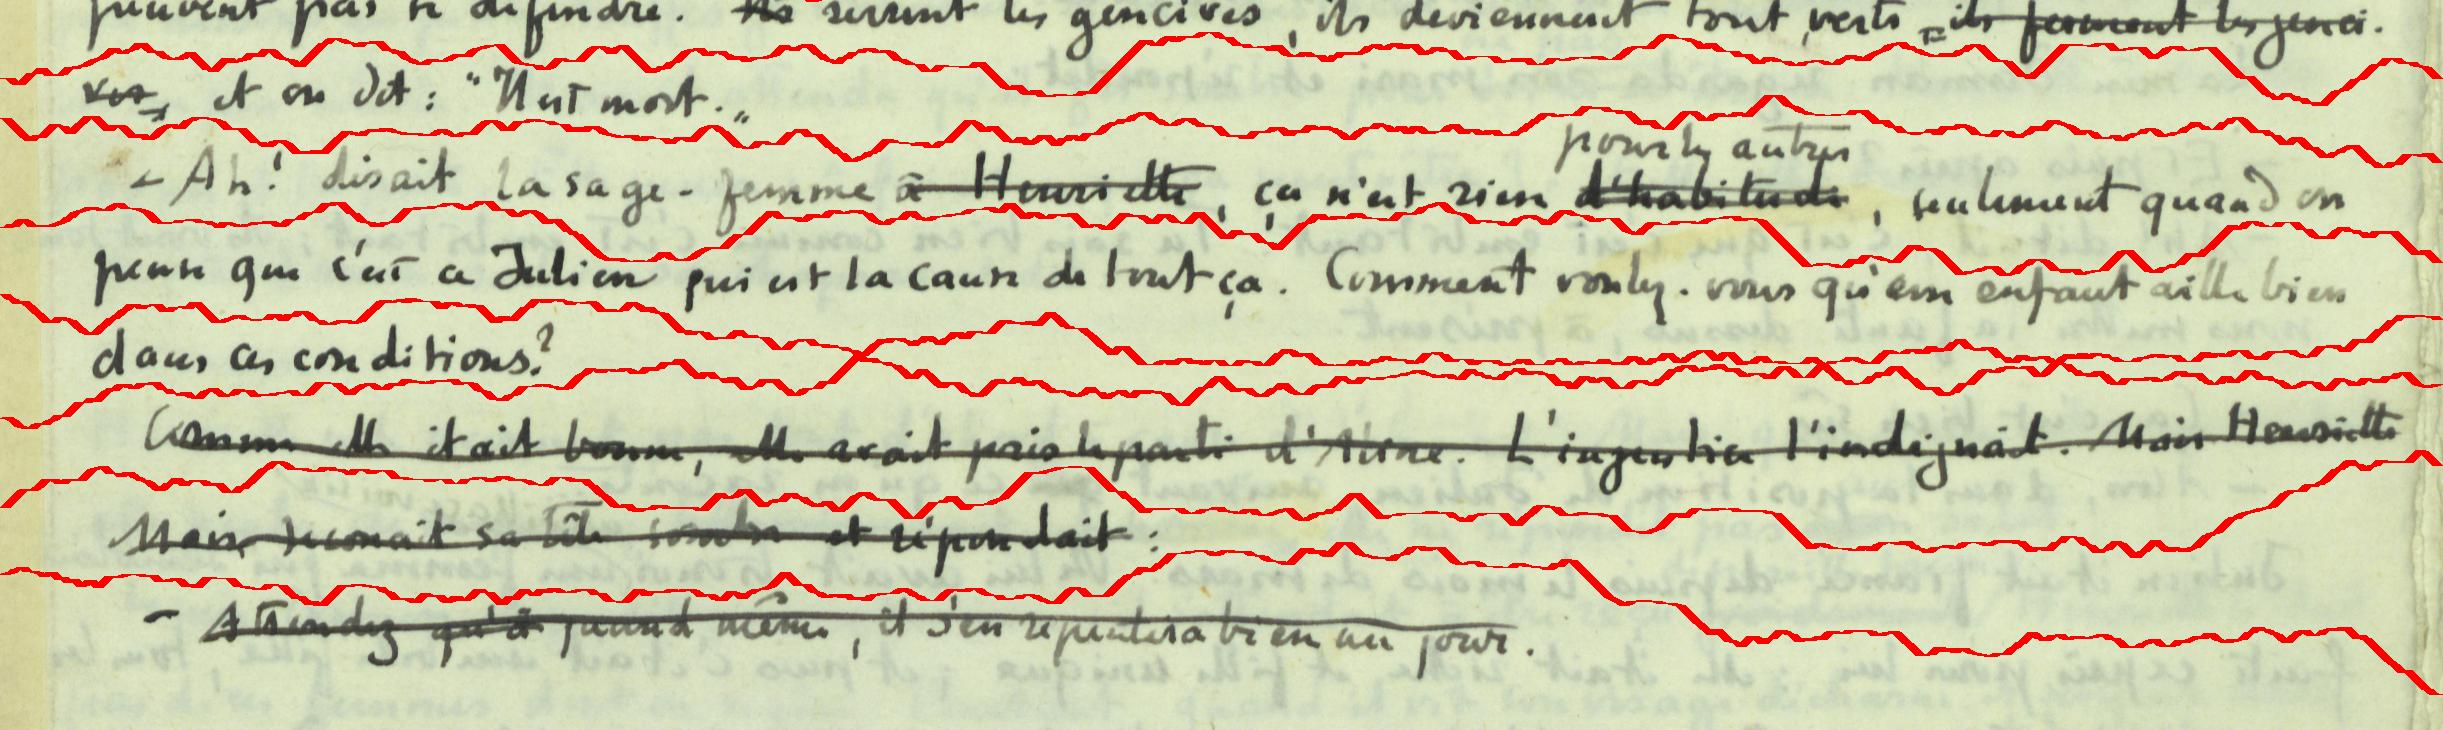
\includegraphics[width=\linewidth]{images/seams.jpg}
	\caption{Paths dividing a text block into lines. (from \cite[figure 5a]{arvanitopoulos2014seam})}
        \end{subfigure}
        \begin{subfigure}[t]{7cm}
        \centering
        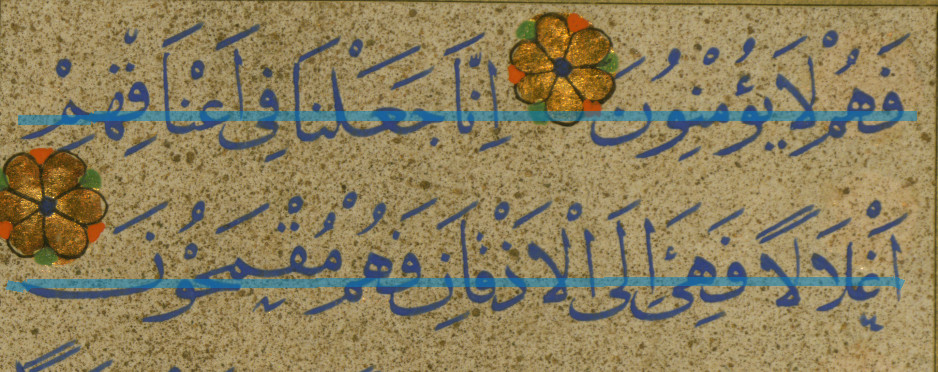
\includegraphics[width=\linewidth]{images/bl.jpg}
	\caption{Baselines (detail of Walters W.578 fol. 5a)}
        \end{subfigure}
        \begin{subfigure}[t]{7cm}
        \centering
        \includegraphics[width=\linewidth]{images/bbox.jpeg}
	\caption{Bounding box around a line (detail of Penn Libraries CAJS Rar Ms 132 fol. 53v)}
	\label{fig:intro_bbox}
        \end{subfigure}
	\caption{Principal representations of lines}
        \label{fig:intro_para}
\end{wrapfigure}

The prevalent paradigm since the development of segmentation-free text
transcription that is able to recognize a sequence of characters at once has
been text line segmentation. While the \emph{what} is evident, the
representation of the text lines is of more interest. The three principal
representations with spread in both research and practical applications are
paths, bounding boxes, and baselines (see figure~\ref{fig:intro_para}).
Axis-aligned bounding boxes, i.e. a bounding box whose edges are parallel to
the image boundary, which contains all the textual content of a particular line
and have an, often implicit, orientation are the most basic practical way to
encode a text line.  One of the benefits of this representation is that
rectangular boxes are a natural fit to the rectangular line strips ingested by
text line transcription methods, and therefore require only minimal processing
in the transcription method. There is a wide array of methods which fit
machine-printed and handwritten text to bounding boxes such as those described
in ~\cite{marti2001influence,papavassiliou2010handwritten} or the LA module in
the OCRopus system~\cite{Breuel03highperformance}. In general, these text line
segmenters struggle with slanted or curved texts, either natural or as a result
of the digitization process, and require the aforementioned preprocessing to
eliminate skew and warping but are inherently unable to accurately segment
multi-oriented and highly curved text. A minor extension implemented in the
Tesseract LA module which increases the versatility of the text line model is
to allow rotation of the text bounding box in combination with an explicit
orientation detection algorithm~\cite{smith2007overview}.

Paths are a flexible alternative which allow the segmentation of slanted and
curved lines with relative ease. They encode blocks of lines that are roughly
in the same orientation through a series of separating linear or non-linear
paths. This representation has one drawback: segmenting a page document into
blocks can already prove to be a challenge. Early methods utilized projection
profiles~\cite{antonacopoulos2004document}, at times piecewise to improve
segmentation of curvature~\cite{zahour2001arabic}. More recent approaches tend
to treat path finding as an optimization problem using the Viterbi
algorithm~\cite{tseng1999recognition} or seam carving~\cite{arvanitopoulos2014seam,zhang2014text}. Notwithstanding the fact that this
approach is superior to using bounding boxes to ensure tight bounds around
curved and/or slanted lines, the above-mentioned block segmentation challenge
prevented its dissemination, and it has never been implemented in any
mainstream OCR engine. It should be noted, however, that the
Aletheia~\cite{6065274} document analysis system implements human-triggered
path-based line segmentation.

Baselines are currently the state of the art for text line segmentation in
highly challenging historical documents. The baseline is an imaginary line
which letters rest on, although letters frequently have parts (called
descenders) that dip below it. It is a fairly common concept which exist in a
large number of alphabetic writing systems, although certain scripts (e.g.
Hebrew, Tibetan, or Bengali) are written with a hanging base or topline
instead, and most logographic scripts such as Chinese do not have any in the
strict typographic sense. In spite of these variations, approximations can
often be systematized well enough to allow the processing of most scripts using
a baseline LA method.

Representing text lines by their baseline has one major advantage: the model
can accommodate arbitrary curvature by defining the baseline as a simple
polyline, i.e. a sequence of straight line segments. Apart from being able to
express any text written in linear writing systems compactly, baseline
representation has the added benefit of allowing rectification through
projection of the individual polyline segments onto a straight line. However,
there is also one drawback. A baseline alone is not sufficient to extract a
complete text line as it is not known which points around it belong to the line
in question or to adjacent content. As a result, baselines are usually
accompanied with additional bounding polygons. Baseline representation appears
in the literature as early as 1989~\cite{srihari1989analysis}. However, it went
largely unnoticed until recently, except for a few segmentation systems~\cite{Breuel03highperformance,smith2007overview} that used baselines internally
for clustering line blobs. Two factors helped their popularization among
researchers. Firstly, \cite{romero2015influence} showed that bounding polygons
had only but a small impact on transcription error rates, although this
certainly does not hold true for all historical documents. Secondly,
\cite{diem2017cbad} published cBAD, a large dataset annotated with
(poly-)baseline, and an evaluation metric for a ICDAR contest. This was
followed by a larger and more complex dataset in 2019~\cite{diem_markus_2019_3568023}. Since then, the literature has produced a
number of methods
\cite{xu2018multi,quiros2018multi,mechi2019text,oliveira2018dhsegment,romain2019semi,gruning2019two,melnikov2020fast}.
They usually combine a deep neural semantic segmentation method (common choices
are U-Nets and FCNs) with a postprocessing heuristic of varying complexity.
While progress in accuracy levels using the ICDAR contest dataset have been
impressive, practical hurdles remain. Since bounding polygons are not part of
standard evaluation metric, they do not define an algorithm for computing one.
Likewise, the metric does not take line orientation into account and the cBAD
dataset is almost exclusively made of upright lines. As a result, there is
neither academic incentive nor any datasets available to develop baseline LA
methods that are able to determine line orientation effectively. Currently, two
OCR systems include trainable baseline LA systems: Transkribus and Kraken (see
chapter~\ref{ch:kraken}), to which must be added support in the eScriptorium
VRE and the OCR-D workflow engine, via the Kraken module.

Other text line representations do exist but they are rarely used in practice.
Pixel labelings and bounding polygons are relatively easy to produce using deep
convolutional ANNs for semantic \cite{pastor2016complete,alberti2019labeling}
or instance segmentation \cite{prusty2019indiscapes}. However, they require
tedious training data acquisition. In addition, in the case of semantic
segmentation-based methods, separation between close lines can be problematic.
Furthermore, without an additional way to determine line orientation or
estimate line curvature, text recognition on rotated and highly curved purely
polygon-bounded lines affects recognition accuracy negatively. This is due to
the fact that lines cannot be effectively normalized to the rectangular line
image strips processed by text transcription methods. 

Some ancillary tasks are also associated with layout analysis. Region
segmentation (also known as page segmentation or zoning) divides a document
image into semantic regions such as main text, decoration, illustration, \dots.
Its output has several applications: to improve the OCR engine’s final textual
output through semantic annotation; to restrict the range of valid output in
other tasks, e.g. by only providing regions of interest to the text line
detector or by limiting the text transcription method to numerals in a postal
code field; or to increase the information available to algorithms for reading
order determination. 

Region segmentation is well-established as a task. There are hundreds of
hand-crafted region segmentation algorithms. They are often optimized for
particular use cases and employ various filtering~\cite{PAVLIDIS1992484},
cutting~\cite{ha1995recursive,kruatrachue2005fast}, and
clustering~\cite{drivas1995page,kise1998segmentation} techniques. As for text
line segmentation, the capabilities of deep convolutional ANNs have made them a
popular choice, and since 2018 a number of publications have focused on this
task~\cite{wick2018fully,oliveira2018dhsegment,xu2018multi,quiros2018multi,he2017multi,chen2017convolutional,monnier2020docextractor}.
A number of systems such as \cite{oliveira2018dhsegment} (U-Net),
\cite{xu2018multi} (FCN), and \cite{quiros2018multi} (GAN with custom CNN) have
implemented an attractive proposition: the possibility to perform both baseline
detection and region segmentation with the same network architecture, or even
the same model \cite{quiros2018multi,xu2018multi}. Certain OCR engines have
started to incorporate neural region segmentation, for instance
anyOCR~\cite{bukhari2017anyocr}, Transkribus, or Kraken. Other systems (e.g.
Tesseract or OCR4all) retain heuristics for this purpose.

Reading order determination (ROD) is an integral part of layout analysis,
albeit it is often overlooked. While systems as described above detect layout
structure, they fail to give any information as per how layout elements are
related logically.  The reading order (i.e. the order in which human readers
will read textual and non-textual components) constitutes one of the most
important logical structures and is critical to understanding a document. It
may sound simple at first, as most modern documents are read following a simple
top-to-bottom order. However, there is a large body of documents for which this
is no trivial matter. Newspapers, for example, contain articles spanning
multiple columns and pages; scholarly editions have critical apparatus which do
not obey the normal reading order; and historical manuscripts often display
extensive marginal notes, interlinear additions, and parallel texts. The
literature on the topic is sparse, in particular when compared to many other
DIA tasks. As a matter of fact, the current state of the art has not evolved
since the early 2000s in any substantial way. \cite{nagy1984hierarchical,ishitani2003document,meunier2005optimized} generate
a region tree with X-Y cuts which is subsequently ordered using simple
heuristic rules (top-to-bottom, left-to-right). \cite{Gao} incorporates
language modelling to determine likely text block sequences in newspapers.
\cite{Breuel03highperformance} uses topological sorting to sort individual text
lines on a page. \cite{AielloIJDAR2002} utilize decision trees that incorporate
both spatial and linguistic features, so as to fit to a complex document
understanding model. A partially trainable system using linear programming to
reconcile user-defined constraints is proposed in \cite{malerba2008machine}.
Despite the fact that some of the above methods are indeed intended for highly
complex documents, all of them make assumptions regarding the spatial ordering
of lines which are ill-suited to many historical documents. However, graph
neural networks have shown promise in logical document structure
analysis~\cite{dejean2019versatile} and might be adapted for ROD in the future.

ROD implementations in OCR engines mirror the current state of the art in
research. OCRopus and Kraken use \cite{Breuel03highperformance}. Tesseract
employs a simple rule-based algorithm described in \cite{5277715}. The OCR-D
workflow engine does not treat ROD as a separate task, instead relying on the
implicit order provided through the respective LA modules.

\subsection{Transcription}

As described in section \ref{s:la}, conventional OCR systems were constructed
around character classifiers. Character classifiers require accurate character
segmentations, which are frequently difficult to obtain for historical,
degraded, and cursive text. To solve this problem, different segmentation-free
methods have been proposed. They recognize one sequence of characters (e.g. a
word or a line) at a time. It should be noted that if the term
segmentation-free is commonplace in the literature, it only applies to the
input data and the training process. This is due to the fact that it is often
possible to extract segmentation as well as estimates of character locations
from their output, as an implicit segmentation is performed internally.

It was via the adaptation of HMM-based methods used in speech recognition that
the earliest approaches, able to both perform sequential classification and to
produce an hypothesis for a possible segmentation, were designed
\cite{kaltenmeier1993sophisticated,rigoll1996comparison}. Such approaches can
be trained easily using Expectation Maximization. In addition, they allow
straightforward incorporation of domain knowledge such as language models, with
the goal of increasing their capacity to model long term dependencies. However,
most HMM OCR methods operate on feature representations that are calculated on
a sliding window over the text line, as is indeed necessary to reduce the
number of model parameters to avoid severe overfitting. HMM-based methods may
differ widely from one to another, in particular when it comes to the choice of
these types of features, and the literature abounds with descriptions of
different general-purpose and heuristic features. An outline of different
feature extractors, modeling granularity, and language models employed in
HMM-based OCR methods is contained in a 2009 survey~\cite{plotz2009markov}.

The inferiority of HMM-based methods to RNNs trained with CTC loss became
blatantly apparent in 2009, when a CTC trained multidimensional LSTM (MDLSTM)
\cite{graves2008offline} won three contests on French, Arabic, and Persian
handwriting transcription without any language-specific method adaptation.
Because the computational requirements of MDLSTMs for both inference and
training made them unsuitable to large scale applications, and also because
some doubts existed regarding their assumed superiority over
1D-LSTMs~\cite{puigcerver2017multidimensional}, simpler bidirectional LSTMs
(BiLSTM)~\cite{graves2008novel} became the basis for numerous derivations of
the general BiLSTM+CTC schema. The first hybrid convolutional and recurrent
neural network (CRNN) for natural scene text recognition was proposed in
\cite{shi2016end}. Meanwhile, \cite{dutta2018improving} augmented a basic CRNN
with a spatial transformer network block that learned to dewarp input text line
images. \cite{stuner2016cohort} incorporated lexicon verification to control a
cascade of text transcription RNNs. \cite{bluche2017gated} combined novel gated
convolutional layers with a multilayer BiLSTM and CTC loss. More complex
training procedures are sometimes constructed around these methods, for
instance incorporating auxiliary language model losses to adapt a transcription
model to an unseen language \cite{tensmeyer2018language}. Another example is
domain adaptation from synthetic machine-printed to handwritten text with
virtual adversarial training \cite{keret2019transductive}.

In recent years, various attempts were made to find alternatives to RNNs or CTC
for text transcription. Apart from the everlasting search for greater accuracy
and generalization, RNNs (and especially LSTMs) are slow and cannot be
parallelized easily. CTC has the aforementioned limitations, to which one must
add complexity, not to mention that fast implementations suffer from
restrictions such as maximum target sequence lengths. Attentional models such
as \cite{sueiras2018offline,michael2019evaluating,kang2018convolve} replace CTC
with conventional losses. In general, they consist of an encoder and a decoder,
where the encoder produces a feature map.  Through an attention mechanism
(which can be of different types, including content- and location-aware
attention), the decoder can weigh at each decoding step the relative importance
of the different parts of the feature map. The number of times the decoder runs
steps is arbitrary, and characters are output directly from the weighted feature map. It
follows that these methods hardly allow the character sequence to align with
the input image. This contrasts with HMMs and CTC-trained ANNs sharply.
\cite{coquenet2020recurrence} describes a recurrence-free, CTC-trained, gated
convolutional ANN which, if compared to CRNNs, achieves similar (albeit
slightly lower) character error rates. Focusing on the recognition of in-air
handwritten Chinese text, \cite{gan2020air} proposes a system that uses
increasingly strided 1D convolutional layers to achieve large receptive fields
in the feature extractor, quite similarly to non-causal temporal convolutional
networks (TCNs). While the complete ANN architecture includes some final LSTM
layers, an ablation study shows that the TCN on its own achieves error rates
that are similar to a simple two-layer LSTM.

As state-of-the-art hybrid CRNNs trained with CTC loss largely surpass older
HMM-based systems and have existed for a few years, many OCR engines include
(C)RNN+CTC transcription modules. The OCRopus system uses a one-layer
bidirectional LSTM trained with a particular variant of CTC loss, implemented
completely in Python. The latest (fourth) version of Tesseract includes a
dynamically configurable neural networking library which is highly optimized
for inference on CPU. In addition, Tesseract’s default network configurations
include unconventional summarizing LSTM layers that compute local features as
the last time step output of an LSTM layer ingesting a one-pixel-wide vertical
slice of the line, one pixel at a time. The OCR4All system uses the Calamari
text classifier, which implements an ensemble method of confidence-weighted
voting of cross-fold-trained CRNNs \cite{wick2018calamari}. Kraken implements a
configurable neural networking backend with a model specification
language~\ref{app:kraken}, defaulting to a simple six layer CRNN.
anyOCR~\cite{bukhari2017anyocr} uses BiLSTMs trained in a conventional
supervised fashion with CTC, but includes a procedure to harvest imprecise
training data through manually labelled character clusters. It aims to
drastically reduce training data requirements.

\subsubsection{Specialty tasks}

Certain specialty tasks exist without being part of any general-purpose OCR
systems. Either the material they are designed for is too uncommon and
dissimilar to writing systems for natural languages, or the state of the art is
not sufficiently accurate to warrant implementation in practical OCR engines.

Table analysis is a task in DIA whose goal is to detect and recognize both the
contents of a table and its logical structure. Despite a long history of
research in table processing methods which extends far into the early
nineteen-nineties \cite{zanibbi2004survey}, this task is still considered
unsolved even for modern printed tables \cite{gao2019icdar}. There is limited
research pertaining to the processing of historical tabular material. Even
hand-crafted methods that are optimized for a particular table style have high
error rates~\cite{lehenmeier2020layout}. Since table retrodigitization remains
an area of commercial interest in the data entry industry, certain proprietary
OCR engines (e.g. Abbyy FineReader) include table detection and structure
recognition.

Optical Music Recognition (OMR) aims to transcribe sheet music into a
ma\-chine-readable representation. The process is analogous to OCR in many ways;
yet the term OMR remains rather ill-defined. It encompasses output
representations (e.g. MIDI) that one would not traditionally associate with
OCR. In addition, musical notation behaves quite differently from most scripts
used for natural language, as it is a featural writing system whose information
is contained both in the ordered sequences of symbols and their spatial
relationships. Some researchers such as \cite{calvo2020understanding} reject
the categorization of OMR as a sub-type of OCR or \emph{OCR for music} and the
field has developed a number of OMR-specific tasks such as staff processing and
musical information reconstruction that have no equivalent in the domain of OCR
(see \cite{shatri2020optical} for a recent survey of OMR tasks and methods).
For practical purposes, the OCR and OMR research fields are distinct. OCR
engines are not capable of processing musical notation and vice-versa.

Likewise, digital map processing is usually treated separately even when the
goal is limited to textual content extraction. This is due to the fact that
non-text elements make up for a larger proportion of the total writing surface
than most other documents. This makes text finding harder for most LA methods.
However, it should be noted that in comparison to other DIA applications text
transcription in maps can better exploit domain knowledge, as the nature of
naturally-expressed geographical data allows alignment with other maps and
incorporation of toponym
dictionaries~\cite{weinman2013toponym,weinman17geographic,sun2020aligning}.
Complete map understanding requires not only text line detection and region
segmentation layout analysis but also the extraction of cartographic features
such as map symbols and contour lines. Most text LA systems are ill-suited for
this purpose, and it is therefore generally performed using dedicated
segmentation methods such as \cite{uhl2018spatialising,liu2020superpixel}.

\subsection{Virtual Research Environments for DIA, OCR, and Digital Humanities}

Virtual Research Environments encompass a broad range of research support
systems that share common characteristics. They offer a web-based working
environment and are tailored to serve the needs of a \emph{community of
practice} \footnote{Communities of practice as defined in
\cite{wenger1999communities} are individuals that are united in action and in
the meaning that an activity has for them as individuals and as a collective,
i.e. communities are composed of active practitioners who create a community
through self-identification with and exchange on a particular, in our case
scholarly, activity.}. They provide a comprehensive catalogue of tools to
support the targeted community in accomplishing its goals. They are open and
flexible with respect to service offering and lifetime, and promote controlled
sharing of both intermediate and final research results by guaranteeing
ownership, provenance and attribution\cite{candela2013virtual}. They are not
specific to OCR or the humanities and can be designed around all kinds of
research activity.

A number of web-based platforms offer manual or computer-assisted segmentation,
transcription, and recognition for certain categories of material in the
humanities field. However, whether they can be considered actual VREs is open
to question. Most platforms are developed within particular institutional
frameworks as project-specific tools, without active buy-in from practitioners
falling outside well-defined collaborations. This situation explains the lack
of platforms that satisfy all criteria for VREs. In this review, we will relax
the criteria while still limiting our review to tools whose functionalities at
least partially overlap with eScriptorium’s.

Most platforms implement specific methods to suit the needs of a particular
scientific project, and most research projects are of relatively short duration
and seek to solve specific research questions. As a result, in typical settings
dedicated platforms are not concerned with implementing a complete catalogue of
methods to perform an activity fully. They also rarely create a scholarly
community around them, albeit they can be considered as being part of a fabric
of loosely-coupled tools that could be made to interoperate through common data
interchange formats. Crowdsourcing applications for transcription of historical
documents have proved to be a particularly successful type of platforms. Tools
like the Bentham Transcription Desk~\cite{moyle2011manuscript} discard any
automatic processing to retain simplicity in implementation. Such platforms are
rarely openly accessible. In other words, data on which users can perform
activities is predetermined by the platform’s operators; imports are often
already processed extensively through external means. The TypeWright OCR
correction and digital edition creation tool~\cite{typewright} is a good example
of this. The only raw OCR data that it makes available was created by the eMOP
project's internal pipeline. On the other hand, it should be noted that a
fairly large number of platforms accepting the use of arbitrary data do exist.
They are, however, of very limited capability. For instance, \cite{webaletheia}
is a platform whose purpose is to create segmentation ground truth data with
some low-level computer vision assistance. Another example is the
HInDoLA~\cite{trivedi2019hindola} platform, which is solely intended to aid the
layout analysis of palm leafs. LAREX~\cite{reul2017larex} is a semi-automatic
tool for layout analysis of early printed books. It can be interfaced to
external OCR tools through data exports in PageXML format. PoCoTo
~\cite{vobl2014pocoto} is a web service geared towards the postcorrection of OCR
output with language modelling assistance.

When it comes to communities of OCR practitioners in the humanities, the
Transkribus~\cite{kahle2017transkribus} platform comes closest in meeting the
VRE definition. It was designed as a comprehensive platform for computer-aided
layout analysis, transcription and information retrieval. It offers all the
basic tools necessary to the average scholar interested in retrodigitization of
historical handwritten and printed material. Unfortunately, the closed nature
of the platform hampers interested scholars’s capacity to share their work
while being guaranteed ownership of their work. While data can be imported and
exported in standard formats freely, artifacts trained in specific OCR tasks
(i.e. layout analysis and transcription models) with user-created data are
locked inside the platform. Added to the platform’s recently adopted pricing
model, it presents not only a significant deficit of ownership but also a
barrier to the reproducibility of results.

While eScriptorium is not yet feature complete and access to the platform of
the public is currently limited, albeit the source code of all components is
publicly available and a number of instances are set up at different research
groups and institution, it already fulfills the VRE definition. It supports the
full gamut of OCR functions needed for the processing of historical material,
permits users to selectively share the product of their work, and provides
interfaces to import and export all data and workflow-produced artifacts.

\printbibliography[heading=subbibliography]
\endrefsection

\printbibliography[heading=subbibliography]
\end{refsection}
\cleardoublepage
\part{The Arabic Writing System}
\begin{refsection}
\chapter{The Arabic Script}
\label{ch:arabic}
\thispagestyle{empty}
\newpage
\refsection

The Arabic writing system is one of the geographically and chronologically most
widely used writing system in human history. It is the primary script for the
Arabic language, Farsi, Urdu, and multiple others on the Indian subcontinent
and has been used historically to produce texts in Spanish to Chinese.

While there is still some dispute on its exact origins, the scholarly consensus
is that the Arabic script evolved either from Nabatean or Syriac script in the
Middle East over the course of multiple centuries with maturation occuring
during the seventh century CE.  Linked closely to the spread of Islam, a number
of alphabetic variants and calligraphic regional styles developed in the
subsequent centuries. Nevertheless it is far from a purely liturgical script
with a wealth of administrative records, philosophical and scientific
treatises, poetry, \dots existing.

It is therefore of a misnomer to speak of a single Arabic script from the
perspective of DIA research. Persian epics in \emph{nastaʿliq} style on highly
decorated marbled paper have little in common with \emph{naskh} private
correspondence or the angular rectilinear writing of early \emph{kufic} quranic
codices. Each style in combination with the regional preferences and the
context of their utilization presents particular challenges. 

\section{The Principles of the Arabic Writing System}

The Arabic script is an \emph{abjad}, a consonantal writing system. Like
scripts for other semitic languages it only requires that consonants and long
vowels to be written, the reader is supposed to supply the appropriate short
vowels themselves from the context. Short vowels and other marks for features
such as doubling (gemination) and nunation (adding a final n), can optionally
be added (\emph{tashkīl}) but are only systematically used when transcribing
the \emph{qurʼān} or elementary texts for language learners. Like Syriac and
Hebrew it is written from right to left with the exception of numbers which are
written from left to right.

\begin{table}[!htbp]
\begin{minipage}{\textwidth}
\begin{center}
\caption{The 28 letters of the Arabic abjad}
\label{tab:abjad}
\renewcommand*{\thefootnote}{\alph{footnote}}
\begin{tabularx}{\textwidth}{XXXXXp{2.6cm}} \toprule
\textbf{isolated} & \textbf{initial} & \textbf{medial} & \textbf{final} & \textbf{name} & \textbf{transliteration}\\
\midrule
\textarabic{ا} & \textarabic{ا} & \textarabic{ـا} & \textarabic{ـا} & ʾalif & ā\\
\textarabic{ب} & \textarabic{بـ} & \textarabic{ـبـ} & \textarabic{ـب} & bāʾ & b\\
\textarabic{ت} & \textarabic{تـ} & \textarabic{ـتـ} & \textarabic{ـت} & tāʾ & t\\
\textarabic{ث} & \textarabic{ثـ} & \textarabic{ـثـ} & \textarabic{ـث} & thāʾ & th\\
\textarabic{ج} & \textarabic{جـ} & \textarabic{ـجـ} & \textarabic{ـج} & jīm & j\\
\textarabic{ح} & \textarabic{حـ} & \textarabic{ـحـ} & \textarabic{ـح} & ḥāʾ & ḥ\\
\textarabic{خ} & \textarabic{خـ} & \textarabic{ـخـ} & \textarabic{ـخ} & khāʾ & kh\\
\textarabic{د} & \textarabic{د} & \textarabic{ـد} & \textarabic{ـد} & dāl & d\\
\textarabic{ذ} & \textarabic{ذ} & \textarabic{ـذ} & \textarabic{ـذ} & dhāl & dh\\
\textarabic{ر} & \textarabic{ر} & \textarabic{ـر} & \textarabic{ـر} & rāʾ & r\\
\textarabic{ز} & \textarabic{ز} & \textarabic{ـز} & \textarabic{ـز} & zayn & z\\
\textarabic{س} & \textarabic{سـ} & \textarabic{ـسـ} & \textarabic{ـس} & sīn & s\\
\textarabic{ش} & \textarabic{شـ} & \textarabic{ـشـ} & \textarabic{ـش} & shīn & sh\\
\textarabic{ص} & \textarabic{صـ} & \textarabic{ـصـ} & \textarabic{ـص} & ṣād & ṣ\\
\textarabic{ض} & \textarabic{ضـ} & \textarabic{ـضـ} & \textarabic{ـض} & ḍād & ḍ\\
\textarabic{ط} & \textarabic{طـ} & \textarabic{ـطـ} & \textarabic{ـط} & ṭāʾ & ṭ\\
\textarabic{ظ} & \textarabic{ظـ} & \textarabic{ـظـ} & \textarabic{ـظ} & ẓāʾ & ẓ\\
\textarabic{ع} & \textarabic{عـ} & \textarabic{ـعـ} & \textarabic{ـع} & ʿayn & ʿ\\
\textarabic{غ} & \textarabic{غـ} & \textarabic{ـغـ} & \textarabic{ـغ} & ghayn & gh\\
\textarabic{ف} & \textarabic{فـ} & \textarabic{ـفـ} & \textarabic{ـف} & fāʾ & f\\
\textarabic{ق} & \textarabic{قـ} & \textarabic{ـقـ} & \textarabic{ـق} & qāf & q\\
\textarabic{ك} & \textarabic{كـ} & \textarabic{ـكـ} & \textarabic{ـك} & kāf & k\\
\textarabic{ل} & \textarabic{لـ} & \textarabic{ـلـ} & \textarabic{ـل} & lām & l\\
\textarabic{م} & \textarabic{مـ} & \textarabic{ـمـ} & \textarabic{ـم} & mīm & m\\
\textarabic{ن} & \textarabic{نـ} & \textarabic{ـنـ} & \textarabic{ـن} & nūn & n\\
\textarabic{ه} & \textarabic{هـ} & \textarabic{ـهـ} & \textarabic{ـه} & hāʾ & h\\
\textarabic{و} & \textarabic{و} & \textarabic{ـو} & \textarabic{ـو} & wāwʾ & w/ū\\
\textarabic{ي} & \textarabic{يـ} & \textarabic{ـيـ} & \textarabic{ـي} & yāʾ & y/ī\\
%\multicolumn{5}{c}{\textbf{vowel and diacritical marks}}\\
%\midrule
%\textbf{letter} & & & & \textbf{name} & \textbf{transliteration}\\
%\textarabic{َ} & & & & fatḥah & a\\
%\textarabic{ُُ} & & & & ḍammah & u\\
%\textarabic{ِ} & & & & kasrah & i\\
%\textarabic{ْ} & & & & sukūn & zero-vowel\\
%\textarabic{ّ} & & & & shaddah & doubled consonant\\
%\textarabic{ًٌ/ً/ٍ}& & & & tanwīn & nunation marks\\
%\textarabic{ء}  &  & & & hamzah\footnote{\emph{Hamzah} is not considered as one of the canonical 28 letters but can nevertheless occur isolated and notsolely as an diacritic.}  & ʾ\\
\bottomrule
\end{tabularx}
\end{center}
\renewcommand\footnoterule{}
\end{minipage}
\end{table}

The original abjad used for writing Classical Arabic with its twenty-eight
distinctive phonemes contains only eighteen graphemes \emph{rasm}, causing the
same grapheme to represent up to five different phonemes. bāʾ, tāʾ, thāʾ, nūn,
and yāʾ share the same shape and are, depending on their position in the word,
written the same way. These glyphs are distinguished by dots placed above or
below them: one below for bāʾ, two above for tāʾ, three above for thāʾ, one
above for nūn, and two below for yāʾ. Correspondingly, dots are used to
differentiate ghayn and ʼayn, ṣād and ḍād, and jīm, ḥāʾ, and khāʾ. In contrast
to vocalization dotting is mandatory and is present in all but the earliest
Arabic texts. See table~\ref{tab:abjad} for an overview of 

Arabic distinguishes itself from other widely used scripts like Latin,
Cyrillic, or Greek by the lack of a printed form, i.e. a form where letters are
written separately, and only the cursive form exists, albeit a large number of
styles exist. Like cursive forms of other scripts, individual letters change
their shape depending on their position in a word: initial, medial, final, and
independent shapes exist, in addition to more complex placement rules along the
baseline in relation to the adjacent letters. Contrary to the cursive forms of
Latin not all letters can be connected to their previous and following letters,
roughly one fifth do not connect to the following letter. As white space
therefore does not necessarily indicate the beginning of a new word,
calligraphers are largely free to vary inter-word, inter-syllable, and
inter-stroke spacing as desired. On the extreme end, a kind of \emph{scripta
continua} arrises\cite[pg. 15]{blair2006islamic}, abandoning word separation
completely, but even conventional calligraphic practice displays some amount of
spacing variation that can throw off optical character recognition systems.

Unlike many other scripts, Arabic does not know capital and lower case letter
forms and texts produced before the twentieth century CE do not contain
Western-style punctation or layout such as commas, periods, question marks,
paragraphs, \dots Instead particular words and phrases are used to introduce a
new sentence or question, strokes are placed above titles and headings, and a
variety of verse marks and signs aiding in recitation are used in Quranic
manuscripts after the ninth century CE \cite{awad2015evolution}.

The script has been adapted for a fairly large number of other languages, most
prominently Persian and Turkish that do have some additional phonemes. Letter
forms are usually adapted by adding dots to graphemes representing similar
phonemes in Arabic, e.g. the Persian \emph{pe} is derived from \emph{bāʾ} by
writing two additional dots below. Sometimes graphemes were also modified more
directly such as the letter \emph{gāf} which is written by adding another bar
above the letter \emph{kāf}. Similar transformations exist for other languages
with some such as \emph{xiao'erjing}, the writing of sinitic languages in
Arabic script, changing it into a full alphabet by making the marking of short
vowels mandatory or creating additional letters for short vowels. The Unicode
standard alone lists more than a hundred additional graphemes for local
variants of the Arabic script.

\subsection{Text Justification}

As described Arabic does not share many features with other alphabetic scripts
but none of these are a fundamental obstacle to a modern OCR pipeline.  While
the cursive nature was seen as a major hindrance to older methods based on
character classifiers which require accurate segmentation to the character
level, newer segmentation-less methods are largely unaffected by this.
Nevertheless the variability in spacing, even on machine-printed text, is still
the primary source of errors (see section~\ref{s:whitespace}). Unfortunately,
the bundle of techniques employed to justify text, i.e. measures ensuring that
text ends flush with the left end of the writing space, require methods aware
of their function in all parts of the OCR pipeline.

These arose from the proscription of hyphenation, the splitting of words to
facilitate line-wrapping, since the tenth century CE, as justification by
white space alone often results in a visually unpleasing result, a phenomenon
known as rivers in Western typography. Western-style hyphenation is thus only
present in some early Koran manuscripts, albeit without explicit splitting
markers such as hyphens. The most probable reason for its abandonment is the
relatively large impact on legibility, especially when the second fragment of a
word is continued on the subsequent page.

A technique popular with later calligraphers for hanging styles such as the
Persian \emph{nastaʼliq}, in particular for poetry written in hemistichs, is
the stacking or heaping of the last syllable or penstroke above the left end of
the line. This technique is particularly attractive for the Persian language
as many words end in the same letters resulting in negligible impact on
legibility. Similar stacking could be performed inside a line by changing the
location and size of diacritical marks \cite[pg. 14]{blair2006islamic}.

Similarly challenging to OCR systems are dislocated fragments into the margin.
Instead of heaping the last syllable on top of the previous stroke, it is
placed in the margin of a text, similarly to a marginal note. These two
practices add another dimension of complexity to the layout analysis component
of an OCR pipeline. First, the layout analysis system has to be able to
accurately detect these fragments, which the methods presented in
part~\ref{part:la} are certainly capable of, at least with models specifically
trained for the purpose. Secondly, these fragments have to be distinguished
from bona fide marginalia and interlinear notes or translations to be properly
inserted in the flow of text in the output by a reading order determination
algorithm that is aware of their existence. A naïve algorithm assuming text is
ordered from top to bottom will, even if other notes are correctly filtered
through previous classification by the segmenter, insert the fragment before
the text of the line it is associated with, i.e. reverse the order.
Unfortunately, reading order determination is a notoriously under-researched
task in DIA, and although some tentative approaches, such as
\cite{dejean2019versatile} that could serve as a basis for versatile reading
order determination methods, exist, all practically available OCR system
operate on simple heuristics.

Two more practices exist, although their impact on OCR performance should be
modest in most cases. The stretching of the letter body or the connections
between individual letters, interchangeably known as either \emph{taṭwīl} or
\emph{kashida}, although the latter term is reserved in some publications on
typography for the first technique. These are used in most Arabic styles,
albeit their exact placement differs between scripts, not only for
justification but also general highlighting of verse beginnings, heading, etc. 

The second consists of upward curving of the baseline, trading horizontal with
vertical space. For conventional layout analysis methods modelling lines as
either rectangular bounding boxes or undirected\footnote{Undirected in the
sense that there is no definition of the text orientation or direction
contained within the polygon but only a bounding polygon is given.} polygons,
these lines, as slanted lines in general, will often cause a degradation of
results. This can be linked to other lines protruding into the bounding box or
height normalization resulting in insufficient text size as demonstrated in
figure XX. Segmenters founded on the baseline paradigm, like the ones presented
in chapters~\ref{ch:icfhr,ch:hip}, do not suffer from this problem as they
allow projecting arbitrarily shaped lines onto a straight line.

\section{Supports and Production}

A consideration often overlooked in the OCR research community is the question
of supports. While the unique challenges of processing inscriptions in stone or
clay tablets are evident, subtle differences on supple writing surfaces are
usually disregarded. Papyrus and parchment being utilized as writing
material, both were rapidly discarded in favor of cheaper paper after the 8th
century CE. Of particular interest to Computer Vision experts are richly
adorned specialty papers which were often used in high status documents.

In addition, a short examination of the inks, dyes and techniques of
illumination are in order, not only because of the difficulties they cause to
OCR systems but also for the potential of large scale, automatized analysis
across collections DIA methods can offer in the future.

\subsection{Supports}

Paper, parchment, and papyrus are the three principal supports used in the
Islamic world, although the firsts pre-eminence far overshadows the latter two
both geographically and in time.

In use as a support for writing since at least 3000 BCE, papyrus is a
light-colored, smooth, and flexible material manufactured from a three to six
meter high Egyptian water reed \emph{Cyperus payrus}. It is produced by cutting
the stalk of the reed into halves and extracting the pulp as thin strips.
These strips are then arranged into a rectangular sheet consisting of two
perpendicular layers before drying under the sun. The dried sheets are smoothed
with a mallet followed by polishing with a shell or ivory. Sheet sizes varied
considerably but were commonly around 20 and 30cm in width and from 30 to 40
cm in length.

Individual sheets were then glued end to end with the overlapping joints being
again smoothed, before being rolled with the horizontal fibers on the inside.
Like in the pre-Islamic period a roll was composed of twenty sheets but papyrus
would also be sold in smaller pieces, the most common being one-sixth of a
roll. A thicker gauge strip of papyrus called a \emph{protokollon} would be
attached to the top of the roll before use to protect it from wear.

Scrolls were employed up until the early eighth century CE but the majority of
surviving documents are in codex form or single sheet documents~\cite[pg.
30]{deroche2006islamic}. While some literary papyri are known, Arabic papyri
are usually documentary in nature, containing letters, edicts, and contracts.
As papyrus must have been a rather expensive writing material, its use was
rather rapidly phased out after the introduction of cheaper paper and
production ceased in the eleventh century CE \cite[pg.
193-194]{gacek2009arabic}. 

Papyri present two problems to DIA methods. As they age, they darken
considerably, often to the point of making the ink almost illegible, and they
are brittle and fragile, resulting in significant degradation
(figure~\ref{fig:papyrus}). The aging process also increases the contrast
between the fibers complicating the process of distinguishing text from
background. Some hand-crafted binarization methods have been developed in the
past for the highly degraded Dead Sea Scrolls \cite{dhali2017digital,
lavee2013computer} but processing remains challenging. A lesser problem is the
length of papyri in scroll form. While many modern neural network based methods
can be adapted to patchwise operation wit minimal loss of accuracy some
methods, especially layout analysis perform better with global context.

\begin{wrapfigure}{O}{0.7\textwidth}
        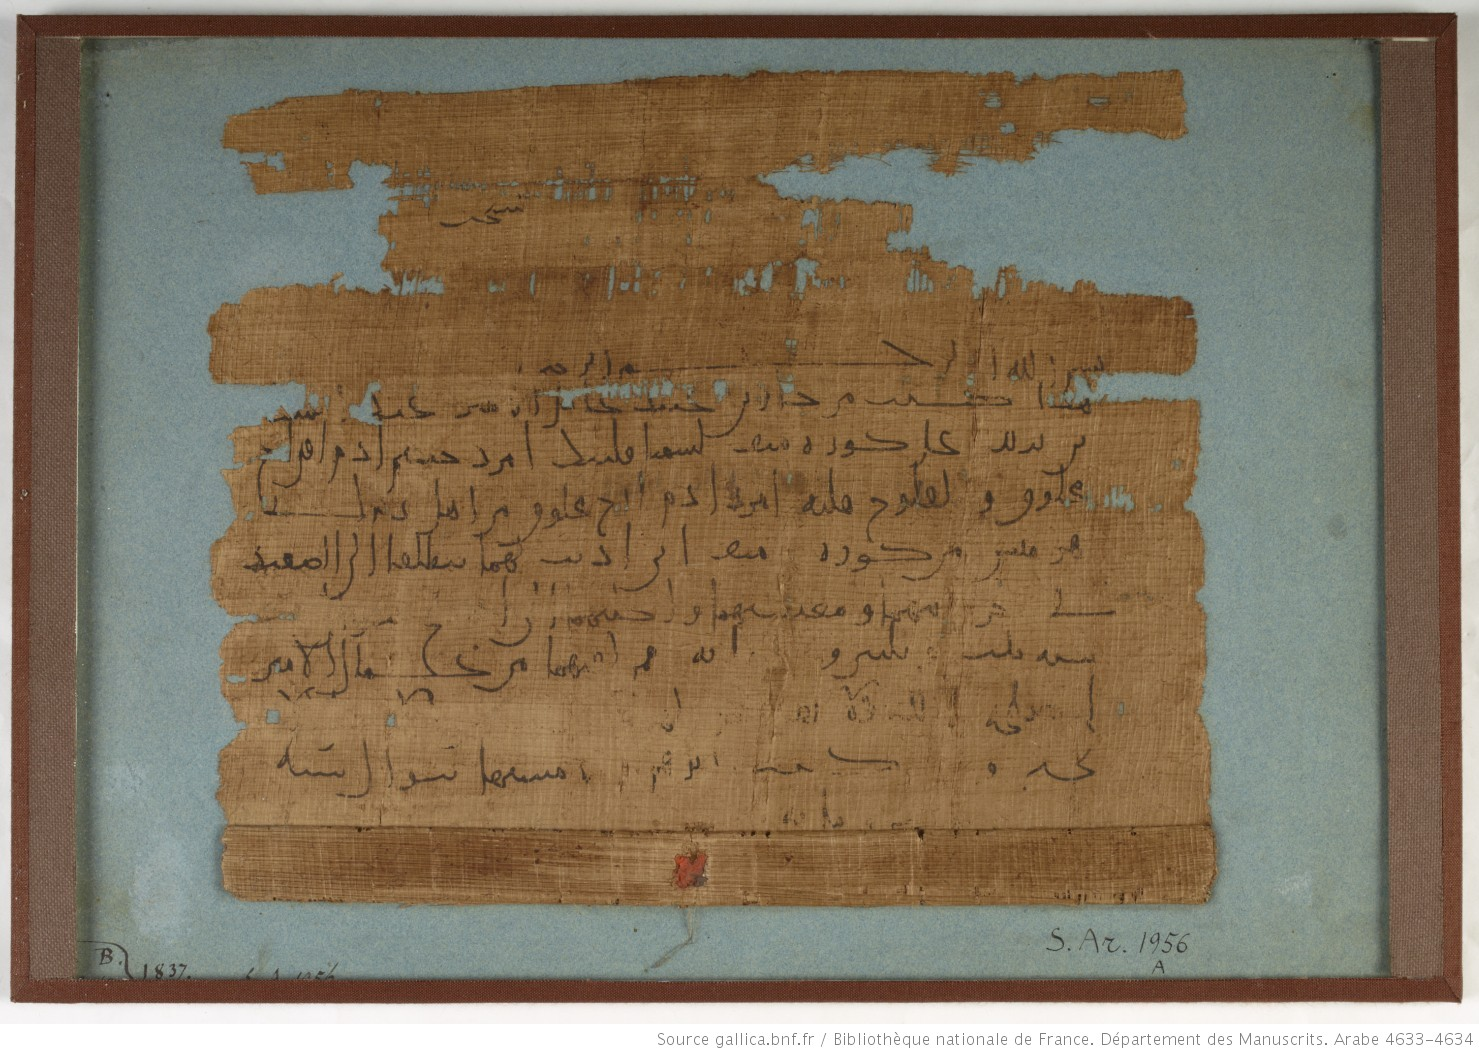
\includegraphics[width=0.68\textwidth]{images/4644.jpg}
	\caption{An Arabic papyrus showing both visible fibers and typical
	deterioration of the writing surface (BnF Arabe 4634).}
        \label{fig:papyrus}
\end{wrapfigure}

The second writing surface in wide\-spread use before the introduction of paper
in the Islamic world was parchment. Parchment is a carefully processed un- or
minimally tanned animal skin; fundamentally it can be procured from a variety
of animals and its production is not limited to a particular geographic area as
papyrus. Goat, calf, donkey, and gazelle skins, although these have never been
corroborated by testing, are mentioned as sources but the most common was sheep
skin~\cite[pg. 44]{blair2006islamic}. Its use in the East extends to time
memorial although no dated Arabic manuscripts from before the ninth century CE
survive~\cite[pg.33]{deroche2006islamic}. 

Parchment is manufactured by first removing the hair from the hide with a basic
solution made from lime or dates. Residual flesh and fat was then scraped from
the flesh side of the hide with a blade, before placing it in a wooden frame to
stretch and dry it. Finally, an abrassive stone was utilized to smooth the
surface and equalize the texture of the flesh and hair side and chalk was
applied to control bleeding of ink. Parchment were sometimes dyed with blue
indigo or yellow saffron; the most famous example of this practice is the Blue
\emph{Qurʼān} from the tenth century CE \cite[pg. 195-196]{gacek2009arabic}.

An important consideration for humanists and computer vision researchers alike,
is the ease with which previously used parchments could be reemployed by
washing or scraping off existing writing. Known as palimpsests, this practice
is attested both in the literature and by several surviving exemplars. There
could be considerably time between between the writing of the first and second
layer and examples of Arabic text over a lower layer written in another script
such as Greek or Syriac exist~\cite[pg. 43-46]{deroche2006islamic}. While the
practice was intended to remove the initial writing as completely as possible,
the lower layer often remains visibile to some extent. Separating the writing
and deciphering both texts is an immensely skilled task which can be aided by
costly multispectral imaging~\cite{easton2003multispectral}. Nevertheless the
problem has not gathered substantial research interest in the DIA community
with results from one of the few publications~\cite{starynska2017methods}
indicating that existing methods would require substantial improvement.
Parchment was also recycled in other ways, being employed in bookbinding and
protective covers to loose quires, similar to papyrus \emph{protokollon}~\cite[pg. 46]{deroche2006islamic}.

Paper was invented in China in 105 CE by the Han courtier Cai Lun. The
traditional account of its introduction to the Islamic world attributes it to a
Muslim victory in July 751 CE on the river Talas in modern-day Kazakhstan.
Chinese papermakers were supposedly taken prisoner after the battle and
dispatched to set up paper mills in Samarqand. Although the actual details of
the story can be disputed, there are etymological hints that the knowledge of
papermaking was received through Central Asia~\cite[pg. 45]{blair2006islamic}.
Paper, significantly less costly than the alternatives, rapidly displaced
papyrus and parchment as the writing surface of choice. Paper mills were
established in Baghdad by 794 CE with its use in the administration of the
Abbasid Caliphate mandated in 808 CE. By the ninth century CE its production
had spread to Egypt, by the tenth century to the Maghreb, and by the twelfth
century to Damascus and Spain~\cite[pg. 51]{deroche2006islamic}.

Apart from economical reasons paper had other benefits: it absorbes ink so
writing could not easily be erased~\cite[pg. 45]{blair2006islamic}, it is less
brittle than papyrus with a more uniform coloration, and can be easily tinted
and decorated.

The availability of an inexpensive writing material in the ninth century
produced a flurry of literary activity in subjects from theology to the natural
sciences. Books were soon copied on paper. Quranic manuscripts remained the
purview of parchment until the late tenth century CE and continued to be used
in the Maghreb and West Africa until the fourteenth century CE.

Description of papermaking in the Islamic world are sparse and unclear. In
general, a suspension of cellulose fibers is drained through a screen and
dried, resulting in a fiber mat called paper. The source of the fibers can vary
considerably: they can either be liberated from virgin plant material through a
combination of heat, beating, and chemical means such as fermentation or acids,
or originate from waste material such as rags, old ropes, etc. They are then
suspended in water to soak and collected and drained in a mold. The dried fiber
mat is called paper. An account from what is now Tunisia describes making paper
from raw flax on a floating screen. Analysis of extant specimens on the other
hand shows that waste materials, such as rags from cotton and linen or ropes,
were primarily used. Before use paper has to be sized with a mixture of
starches and egg white and burnished to prevent the ink from bleeding
excessively~\cite[pg. 44-45]{bloompaper}.

\begin{figure}[h!tp]
        \centering
	\begin{subfigure}[t]{0.3\textwidth}
		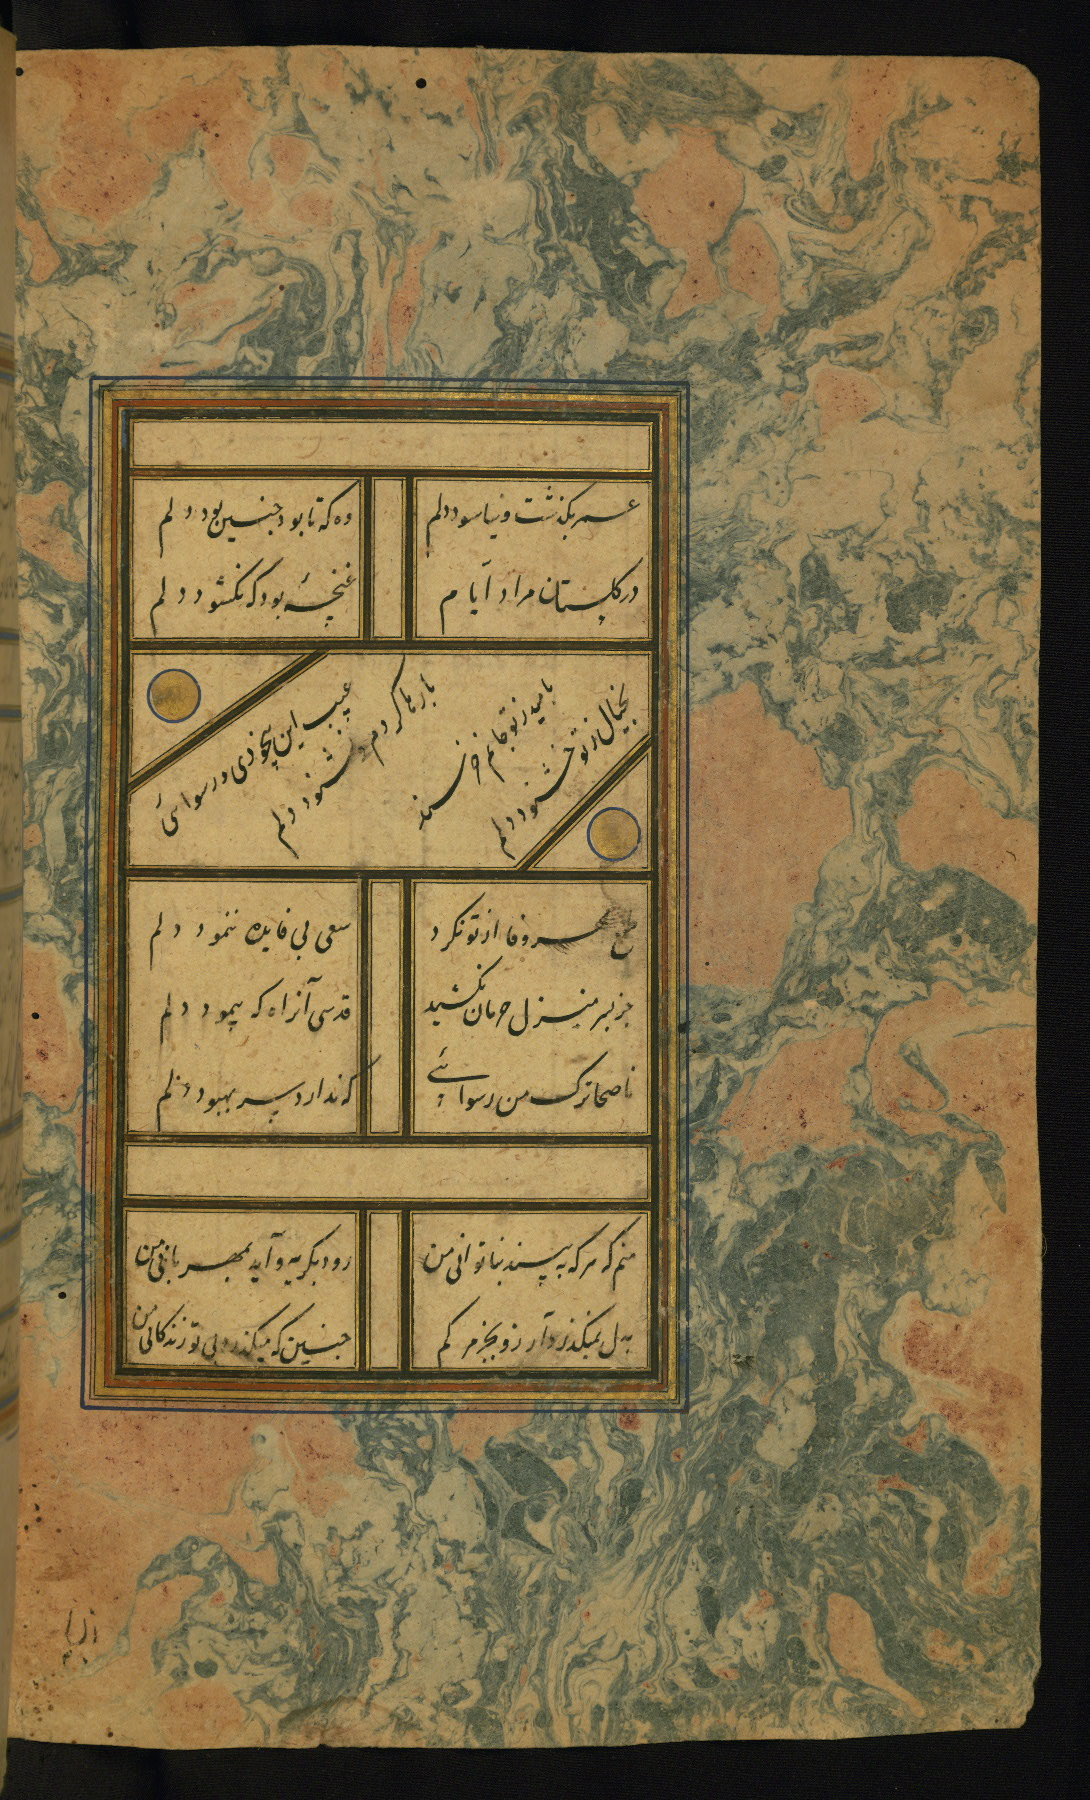
\includegraphics[width=\textwidth]{images/W654_000010_sap.jpg}
		\caption{Example of marbled paper (Walter W.654, fol. 1b)}
                \label{fig:ara_marble}
        \end{subfigure}
	\hfill
	\begin{subfigure}[t]{.3\textwidth}
                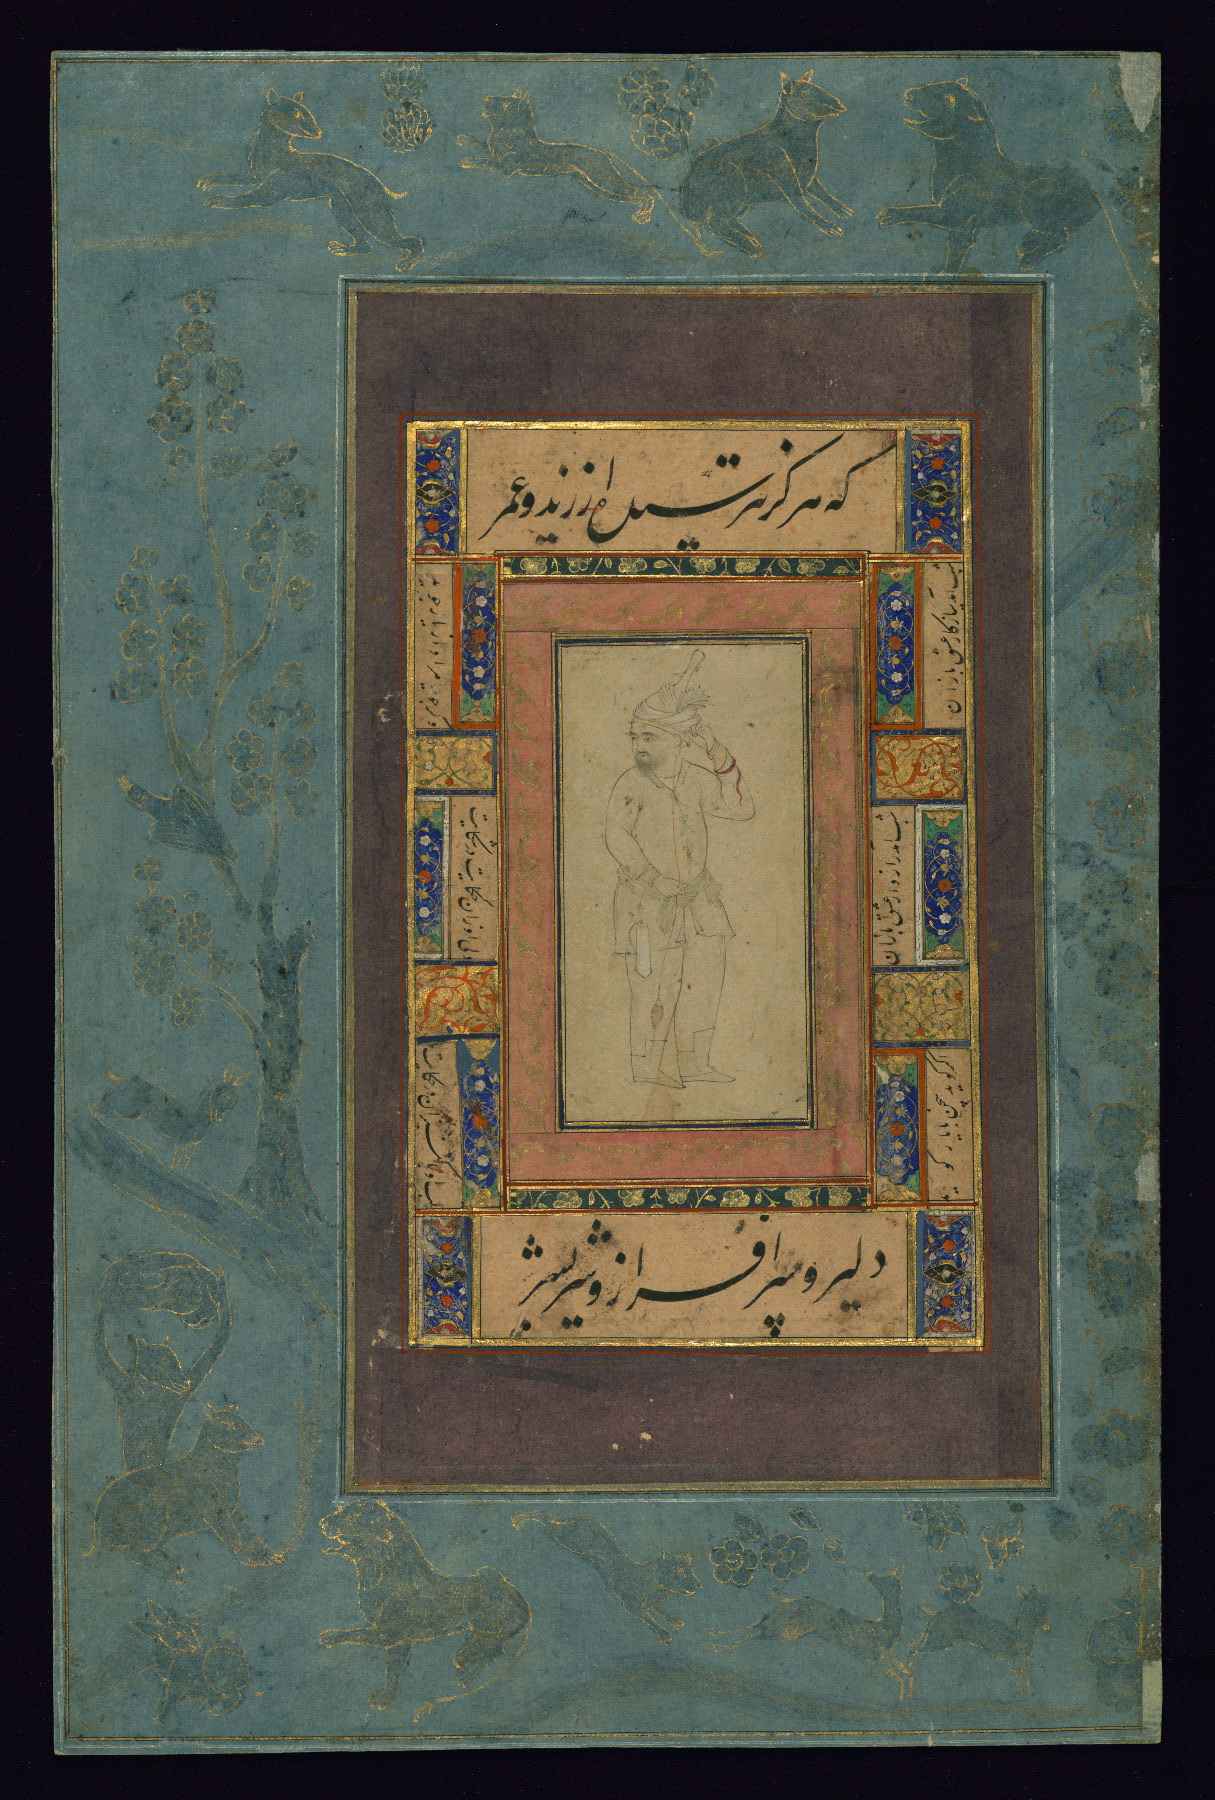
\includegraphics[width=\textwidth]{images/W746_000001_sap.jpg}
		\caption{A page with an outer border made of blue-tinted paper and an inner rose-tinted paper (Walters W.746).}
                \label{fig:ara_blue}
        \end{subfigure}
	\hfill
	\begin{subfigure}[t]{.3\columnwidth}
                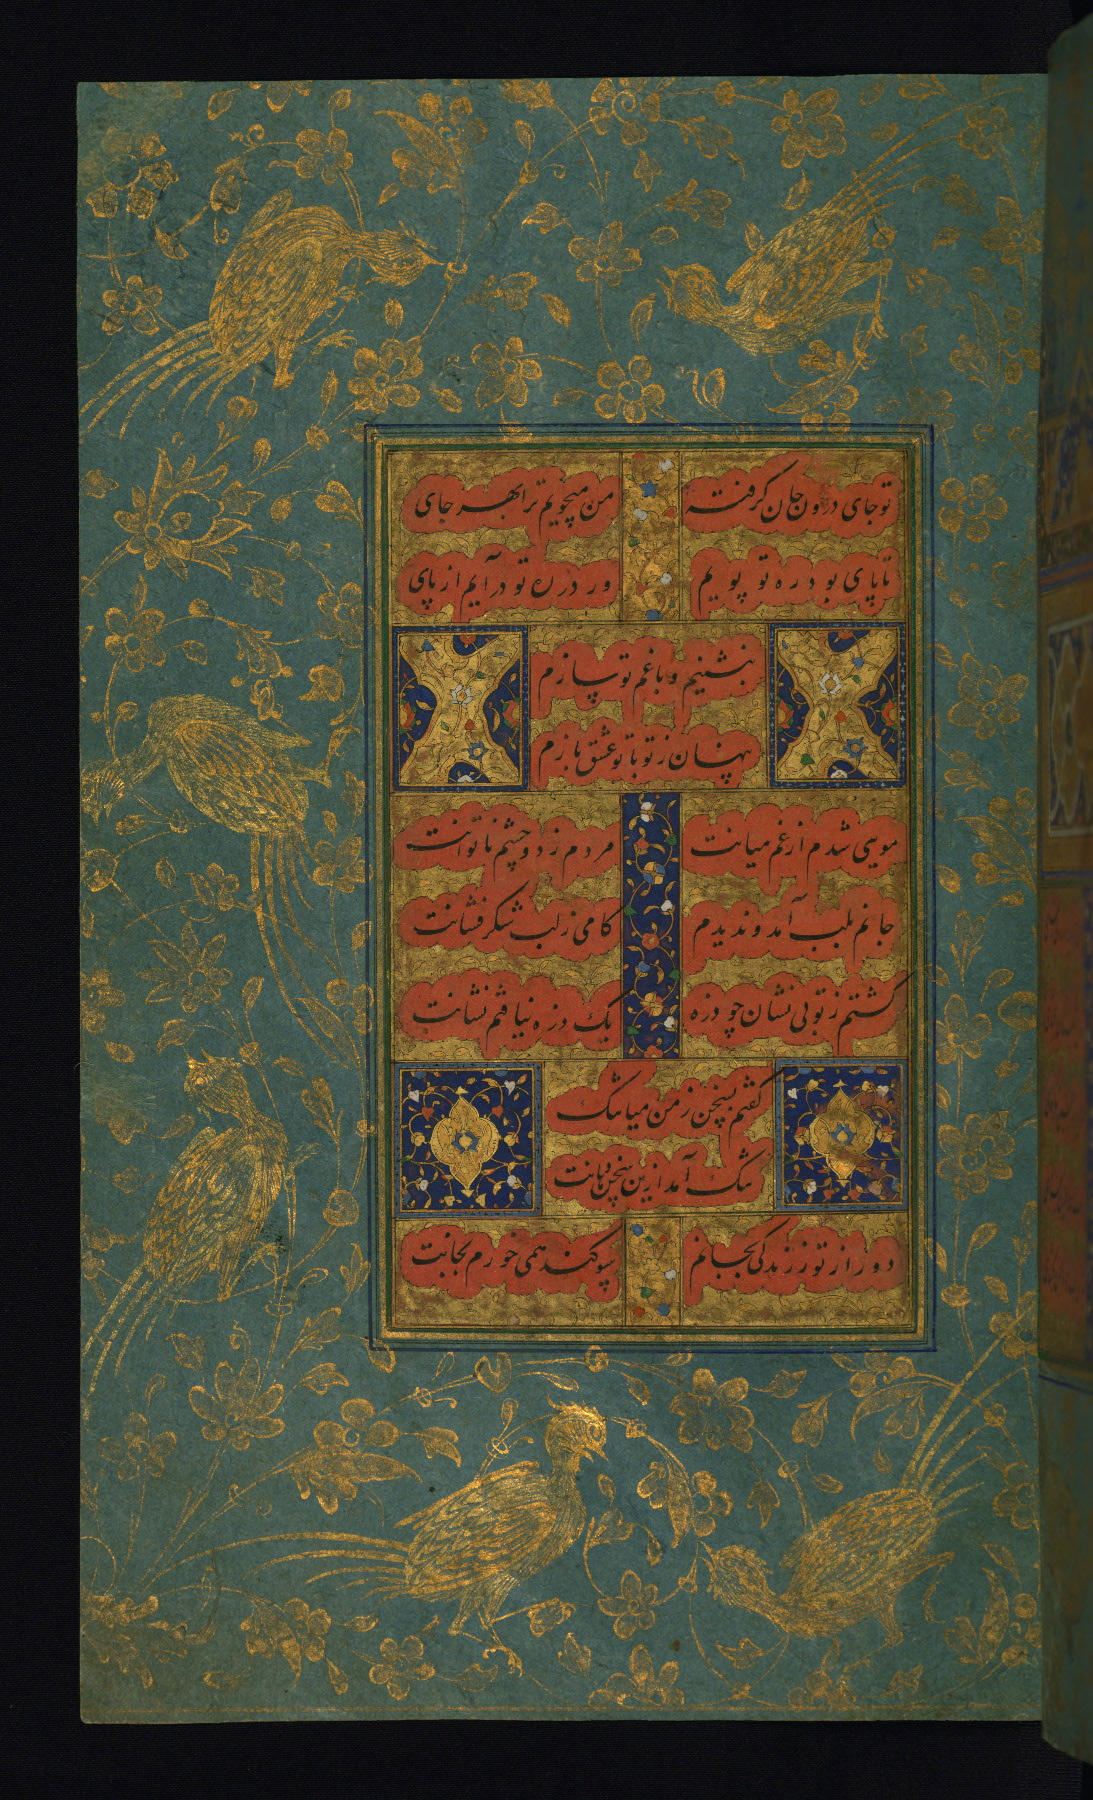
\includegraphics[width=\textwidth]{images/W651_000009_sap.jpg}
		\caption{Illumination in gold on blue-tinted border with text written on orange-tinted paper (Walters W.651, fol. 2a).}
                \label{fig:ara_orange}
        \end{subfigure}
        \caption{Decorated papers}
\end{figure}


A particularly impressive practice that often presents a challenge to modern
DIA methods are specially prepared papers used for many fine manuscripts.
Pre-modern papers retained the color of the source of the fibers, a fact that
was used in European manufacture to produce colored papers, most often various
hues of brown, but could also be tinted or dyed (figure~\ref{fig:ara_blue}).
The preference for tinted papers was probably initially fueled by colored
imports from China but Iranian artists started developing techniques to make
colored, gold-decorated, and marbled papers by the thirteenth century CE.
Popular colors were red or orange, and Persian treatises of the time list a
plethora of recipes to obtain these colors. Gold-sprinkled paper
(figure~\ref{fig:ara_orange}) was utilized throughout the Eastern Islamic lands
by the late fifteenth century CE with even more elaborate gold painting
incorporating arabesques coming into fashion from the sixteenth century onward
at the Safavid, Mughal, and Uzbek courts. Such gold-decorated papers were
mainly used in scrapbook albums of calligraphy and paintings to unify the
disparate contents into a single book. 

Other techniques rising in popularity after the fifteenth century CE are
marbled papers (figure~\ref{fig:ara_marble}) and paper cuts. While the marbling
produced by slipping a sheet of paper over a bath of carefully swirled colorant
cause the same issues to DIA methods as other decorated margins, paper cuts are
likely more complicated.  Cut-out calligraphy, either collage, i.e. placing
cut-out letters on a contrasting background, or decoupage, i.e. mount a sheet
with cut out letters above a differently colored one, allows larger variation
in coloration than purely ink-based writing. Artists were often skilled in more
than one of these techniques and they are often employed together. Works such
as a collection of forty hadith for the Ottoman prince Mehmed in 1540 CE,
contain text in both \emph{taw'qī} and \emph{nastaʼlīq} script, pasted in gold,
white, or light blue on deep-rose or olive grounds. The margins on some pages
are kept plain, others gold-sprinkled, others again marbled~\cite[pg.
52-56]{blair2006islamic}. The sheer variety of printing even contained in a
single manuscript are sure to challenge any DIA system.

\subsection{Writing Instruments and Inks}

The Arabic script is traditionally written with a reed pen whose front had been
trimmed with a special pen knife to create a nib. Depending on the desired
width of the script the nib was slit one or more times at its end. Multiple nib
cuts existed. While straight and oblique cuts changed the thickness of strokes
at certain angles, the association of cut angles and scripts seems to have been
largely a matter of scribal preference~\cite[pg. 42]{gacek2009arabic}.

Brushes were primarily used in the process of decoration, such as paintings in
the margins or gilding. Chinese muslims developed the rounded, flowing
\emph{ṣīnī} script in the fourteenth century CE to adapt Arabic writing to the
instruments and conventions of Chinese calligraphy, even going so far as to
change the directionality of the writing to top-to-bottom in some
cases~\cite[pg. 29-30]{ghoname2012sini}.

Of more pertinence to the application of document image analysis than the
writing instruments are the inks and pigments employed in writing. Three kinds
of black or brown inks were commonly used: carbon-based inks, so-called mixed
inks, and iron gall inks, although compound inks were common in the medieval
period~\cite[pg. 62-63]{blair2006islamic}. All were known in the area of the
later Islamic lands since antiquity. Carbon inks are attested as far back as
the second millenium BCE in Egypt while the first recipes for mixed inks dating
to the third century BCE and iron gall inks being in use by the fifth century
CE~\cite{christiansen2017manufacture}.

Carbon inks, more commonly known as India inks, are composed of fine soot or
finely ground charcoal mixed with some kind of binder, such as oil, gums, or
shellac. For portability they were often carried as a solid stick that is
ground and mixed with water before use. The main source for carbon used in inks
in the muslim world was from the combustion of vegetable matter such as rice,
olives, and chick-peas or various oils. The most common binders were gum arabic
and honey~\cite[pg. 133]{gacek2009arabic}. Inks prepared in this manner adheres
only superficially to the writing surface, can easily be washed off with water
and smudge easily when kept in humid conditions or peels off over time. An
improvement are the so-called mixed inks that are made of carbon inks to which
copper, lead, or iron salts were added. These were intended to increase
adherence to the paper and functioned as drying agents. Iron gall inks do not
contain any carbon and functions by oxidation of the ink once applied to the
paper which forms an insoluble ferric tannate pigment. It is prepared by mixing
tannic acid extracted from gallnuts, vitriol (ferric sulfate), and a binder
such as gum arabic. In contrast to the previous two inks it penetrates the
writing surface and is indelible \cite{christiansen2017manufacture}. Their
major drawback is their acidic nature and fading over time. Manuscripts written
in iron gall ink are often damaged by acid burns to the point of being
illegible to human readers and computer vision methods alike~\cite[pg.
145]{gacek2009arabic}

Colored inks were utilized by scribes and calligraphers as accent colors for
rubrics, vocalization, and other decoration. Red, green, and yellow were most
widely employed. Although the pigments used in the manufacture of these inks
have not been systematically studied, cochineal, vermillion, and red lead
contained in red, lapis lazuli and azurite in blue, and verdigris in green
inks. There is also substantial regional differentation with different pigment
and color use between the east and the west~\cite[pg. 63]{blair2006islamic}.
Coloration of this kind is largely unproblematic to modern DIA methods,
although pipelines employing binarization will encounter substantial
degradation as the most commonplace binarization algorithms perform quite
poorly on mixed-color texts. Of more universal troublesomeness are metallic
inks, such as in figure~\ref{fig:ara_muhaqqaq}, not for their inherent
illegibility but the low contrast exhibited by scanned documents. Both fine
metals such as gold and silver and copper were used in at least two different
ways: liquid inks, made of metal flakes suspended in a binder~\cite[pg.
225-227]{raggetti2019inks}, and dispersing powdered flakes onto glue which were
subsequently burnished and ringed with other colors. Writing produced with the
latter technique is often liable to degradation as disintegration of the glue
has caused flakes to fall off~\cite[pg. 63]{blair2006islamic}.

\section{Styles}

A large number of formal and informal calligraphic styles have been devised
over the centuries. While informal styles naturally evade uniform
classification, the formal styles can be grouped into ones that are recognized
throughout the Muslim world, such as \emph{naskh}, and ones that are largely
limited to a certain geographical region or only used to write specific
languages, such as the North African and Iberian \emph{maghribi} or the Persian
\emph{nastaʼlīq}  

Arabic styles can be defined by elements such as~\cite[pg. 242-243]{gacek2009arabic}:

\begin{description}
	\item[Line of writing] whether all words sit completely on the
			       baseline, descend onto it as in
			       \emph{nastaʼlīq}, curve upwards toward the end,
			       or are slanted.
	\item[Ascender and descenders] vertical, slanted or curved
	\item[Nib width] especially in relation to script size.
	\item[Shading] i.e. contrast between thin and thick strokes.
	\item[Vocalization] Some scripts require a different pen for vocalization.
	\item[Ligatures] The presence of unauthorized connections between letters.
	\item[Contractions] The presence of assimilated (omitted) letter forms.
	\item[Characteristic letterforms] such as straight, wavy, or slanted \emph{ʾalif}
\end{description}

The two earliest styles that emerged in the seventh century CE are
\emph{ḥijāzī} (figure~\ref{fig:ara_hijazi}) and kufic
(figure~\ref{fig:ara_kufic}. Both are somewhat confusingly named after early
Islamic intellectual centers (Hijaz and the city Kufa in southern Iraq) and a
variety of alternative terms such as Early Abbasid have been proposed. As
canonicalization was fairly low the terms do not refer singular hands but to
families of styles that were used mainly to transcribe copies of the
\emph{qurʼān}. One taxonomy divides them into six and four groups for the kufic
and \emph{ḥijāzī} family respectively. Either is notably more angular than
later round styles.  Hijazi being in use from 650 CE it was surplanted by kufic
by the beginning of the eighth century CE. While elaborate, highly decorated
manuscripts in the kufic style survive, the number of surviving Hijazi
fragments is very low and their appearance is utilitarian \cite[pg. 98,
124]{gacek2009arabic}.

\begin{figure}[h!tp]
        \centering
        \begin{subfigure}{\textwidth}
		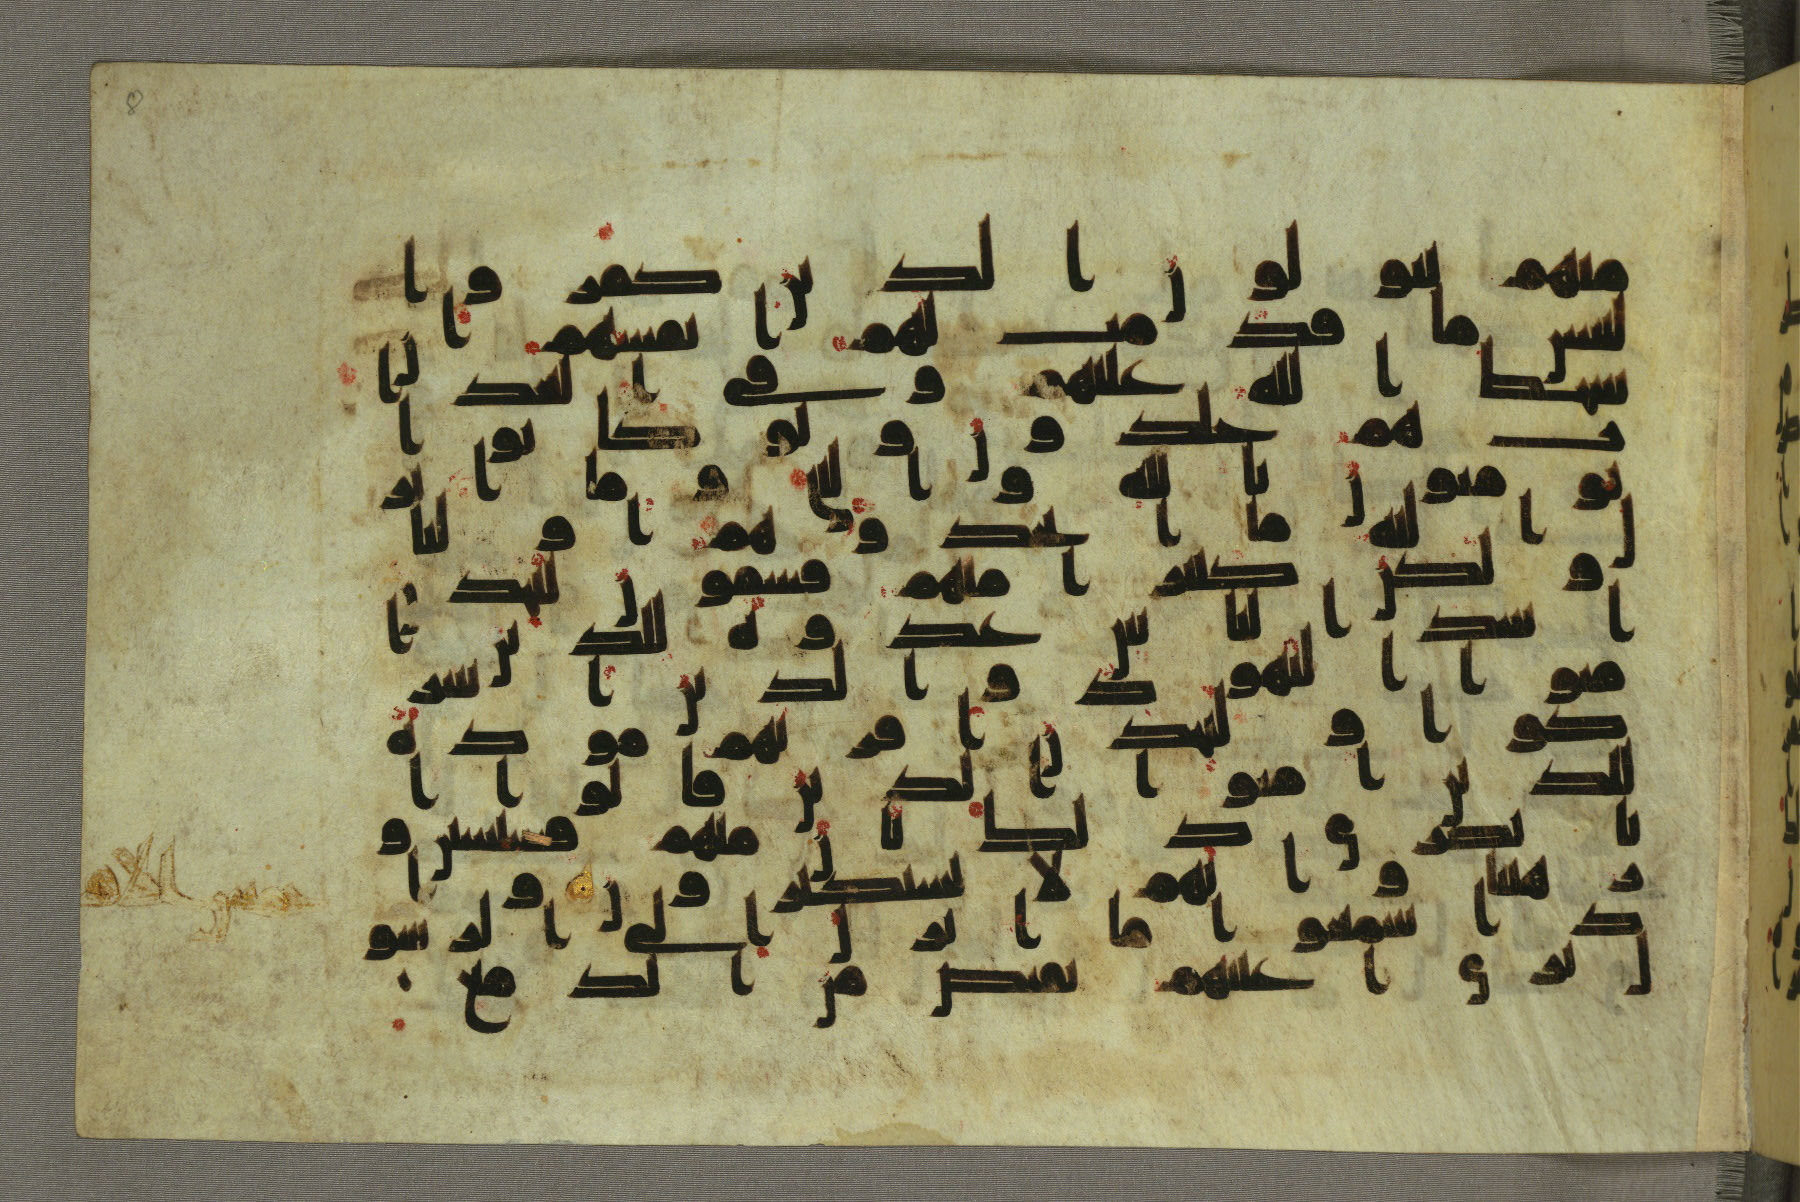
\includegraphics[width=\textwidth]{images/W552_000024_sap.jpg}
		\caption{Ninth century CE \emph{qurʼān} in Kufic or Early Abbasid script (Walters W.552, fol. 8a)}
                \label{fig:ara_kufic}
        \end{subfigure}
        \vskip\baselineskip
	\begin{subfigure}[t]{.48\textwidth}
                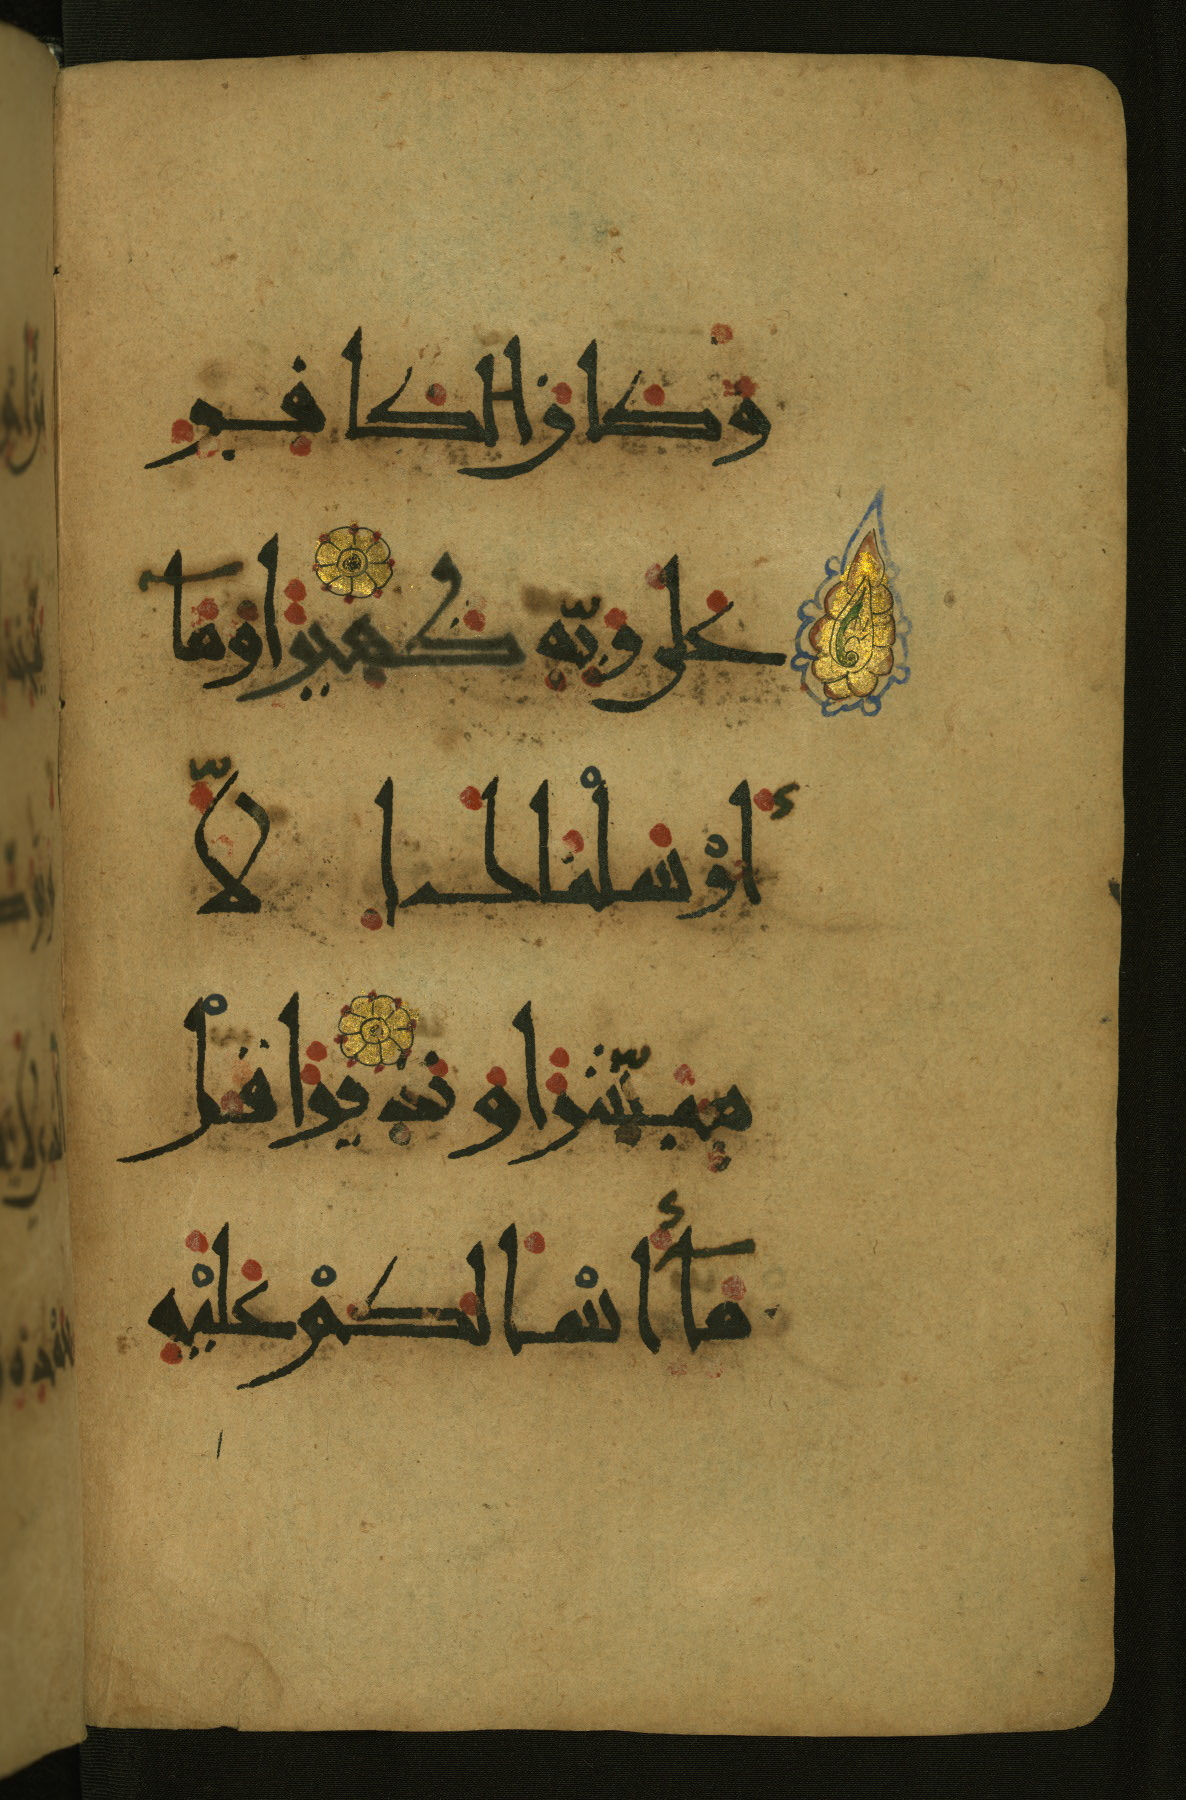
\includegraphics[width=\textwidth]{images/W555_000024_sap.jpg}
		\caption{Twelfth century CE \emph{qurʼān} in broken cursive or New Abbasid script (Walters W.555, fol. 10b)}
                \label{fig:ara_broken}
        \end{subfigure}
	\hfill
	\begin{subfigure}[t]{.48\columnwidth}
                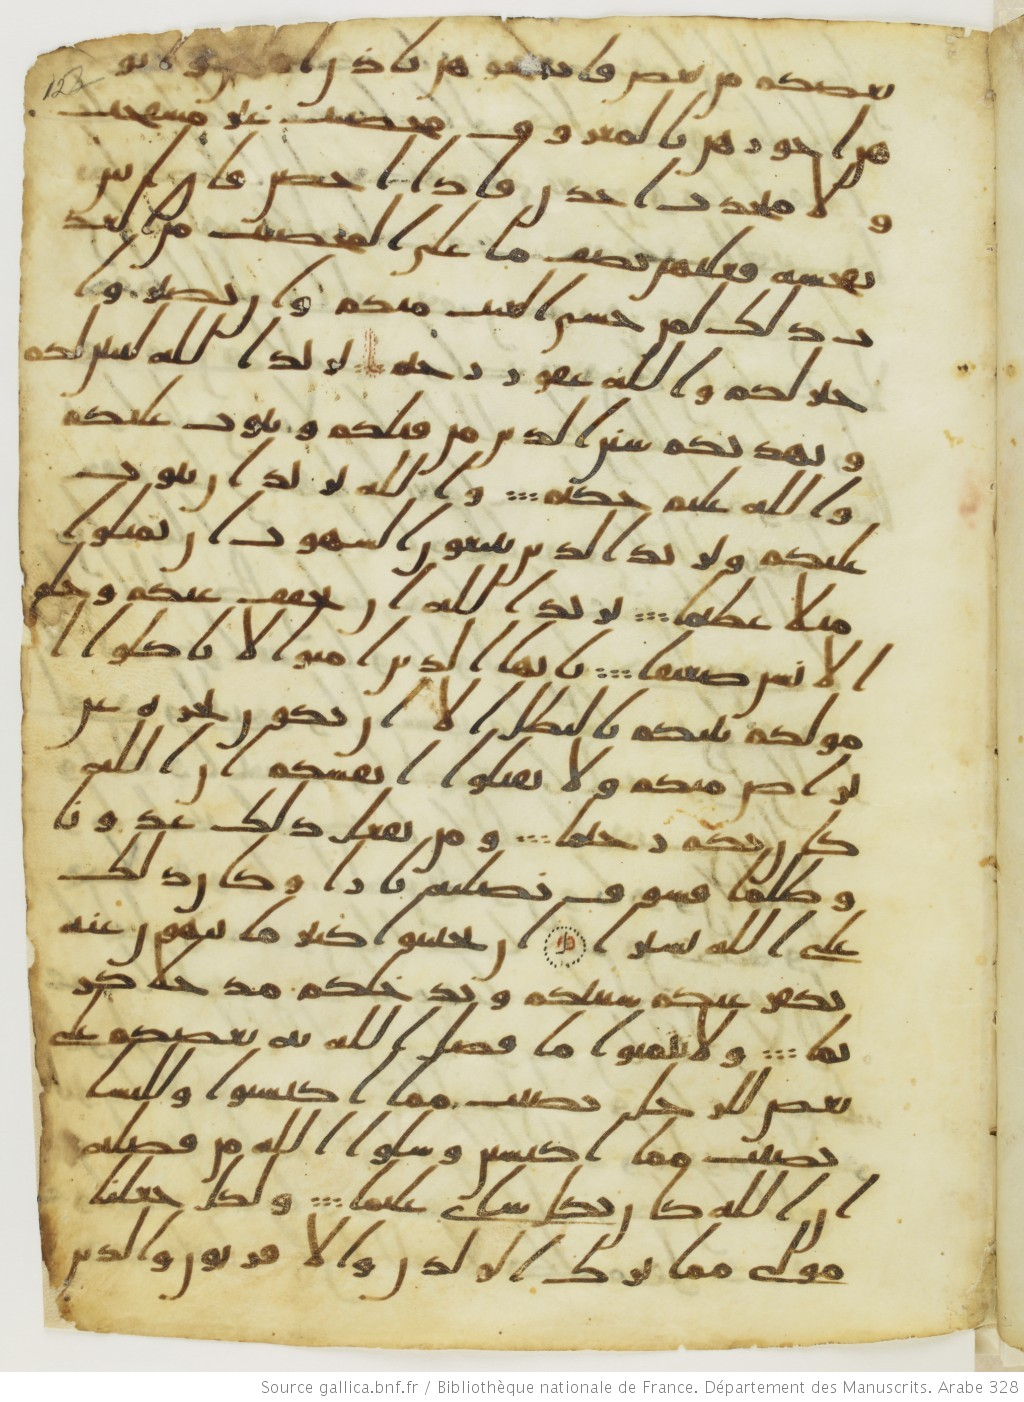
\includegraphics[width=\textwidth]{images/Coran__btv1b8415207g_31.jpeg}
		\caption{Seventh century CE \emph{qurʼān} in \emph{ḥijāzī} script (BnF Arabe 328, fol. 12r)}
                \label{fig:ara_hijazi}
        \end{subfigure}
        \caption{Early Arabic styles}
\end{figure}

By the tenth century CE the use of kufic in high status manuscripts began to be
replaced by a style known under a variety of names such as Eastern kufic, New
Abbasid Style, and broken cursive~\cite[pg. 144]{blair2006islamic}
(figure~\ref{fig:ara_broken}). This style was dominant into the thirteenth
century CE for copies of the \emph{qurʼān} when it was relegated to ornamental
purposes such as titles and headings. As with older styles, it represents not a
single hand but at least two different groups. The main characteristics of this
style is the marked difference between thick and thin strokes \cite[pg.
167-168]{gacek2009arabic}. From this period also dates the practice of using
long \emph{taṭwīl} elongation to mark the start of a new section of
text~\cite[pg. 165]{blair2006islamic}.

\subsection{The Six Pens}

The responsibility for the advancement of the Arabic script until the
thirteenth century CE is traditionally assigned to three great calligraphers:
Ibn Muqlah (d. 940), Ibn al-Bawwab (d. 1022), and Yaqut (d. 1298). The
fundamental development of the period between the tenth and thirteenth century
is the system of proportioned scripts and the canonicalization of the various
rounded styles under this system. Ibn Muqla is attributed with developing the
first proportioned script, \emph{al-khatt al-mansub}, that defined each
letter's dimensions in the unit of rhomboid dots, impressions left by the reed
pen on the writing surface, with \emph{alif} spanning a circle circumscribing
all other graphemes. While this system is most likely only a thirteenth century
CE attempt at reconstructing the hand of the famous calligrapher, as none of
his works survived, Ibn al-Bawwab is credited with canonicalizing the round
chancery scripts in use at the time using this system~\cite[pg. 158-160,
213]{blair2006islamic}. Finally, the popularization of the six proportional
styles known as the \emph{Six Pens} as the dominant scripts in the East falls
during the lifetime of Yaqut~\cite[pg. 251]{gacek2009arabic}.

These six styles are usually paired in three sets of one display (majuscule)
and one text (minuscule) script:

\begin{itemize}
	\item \emph{thuluth} with \emph{naskh}
	\item \emph{muḥaqqaq} with \emph{rayḥān}
	\item \emph{tawqīʿ} and \emph{riqāʿ}
\end{itemize}

\begin{figure}[h!tp]
        \centering
        \begin{subfigure}{\textwidth}
		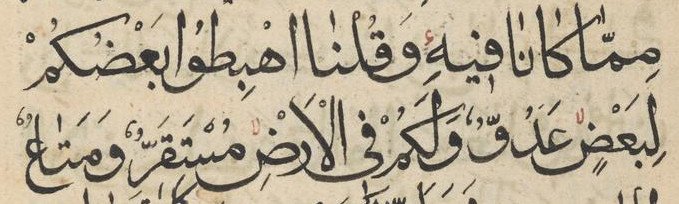
\includegraphics[width=\textwidth]{images/6940_0010_web.jpg}
		\caption{Two lines written in \emph{thuluth} from an undated copy of the \emph{qurʼān} (Columbia University, MS Or 234, fol. 4v).}
                \label{fig:ara_thuluth}
        \end{subfigure}
        \vskip\baselineskip
        \begin{subfigure}{\textwidth}
		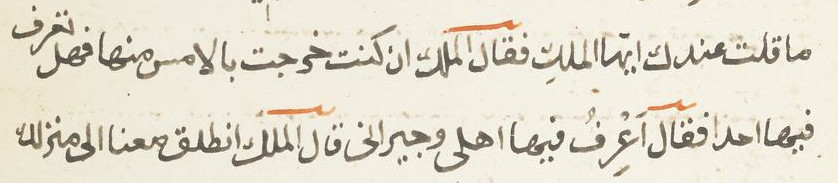
\includegraphics[width=\textwidth]{images/9224_0009_web.jpg}
		\caption{Two lines written in \emph{naskh} from an undated book of quranic stories (Free Library of Philadelphia, Lewis O 170, fol. 5r).}
                \label{fig:ara_naskh}
        \end{subfigure}
        \vskip\baselineskip
        \begin{subfigure}{\textwidth}
		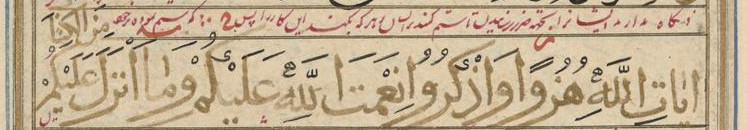
\includegraphics[width=\textwidth]{images/6937_0054_web.jpg}
		\caption{Central line in \emph{muḥaqqaq} in gold of a bilingual
		Arabic and Persian copy of the \emph{qurʼān}. The red line
		above is part of the interlinear Persian translation in
		\emph{nastaʼlīq} (Columbia University, Ms Or 222, 23r).}
                \label{fig:ara_muhaqqaq}
        \end{subfigure}
        \vskip\baselineskip
        \begin{subfigure}{\textwidth}
		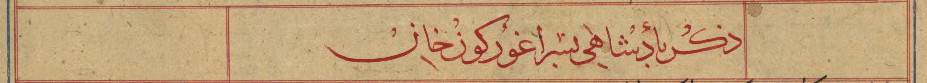
\includegraphics[width=\textwidth]{images/W676_000004_sap.jpg}
		\caption{Chapter heading written in  \emph{tawqīʿ} script from a fifteenth century CE Timurid history (Walters W.676, fol. Bb).}
                \label{fig:ara_tawqi}
        \end{subfigure}
        \vskip\baselineskip
        \begin{subfigure}{\textwidth}
		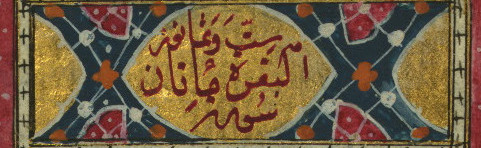
\includegraphics[width=\textwidth]{images/W567_000005_sap.jpg}
		\caption{Heading in \emph{riqāʿ} script of a nineteenth century CE \emph{qurʼān} copy (Walters W.567, fol. 2a).}
                \label{fig:ara_riqa}
        \end{subfigure}
	\caption{Samples of five of the Six Pens}
\end{figure}


\emph{Thuluth} (figure~\ref{fig:ara_thuluth}) is an ancient chancery script
although its exact features are unknown prior to its reform to the proportioned
script system in the eleventh century CE. Its most notable properties are
descenders which fall far below the baseline and curve upwards again for
certain letters, hairlines, and many contracted letterforms. As a display
script its letter are large but horizontally compact. In administrative use it
was utilized for important documents while in codices it was used mainly for
titles and chapter headings~\cite[pg. 275]{gacek2009arabic}.

\emph{Naskh} (figure~\ref{fig:ara_naskh})  is the most widely used bookhand of
the Islamic East. It is a serifless script without unauthorized connections
between letters, long ascenders, and short descenders. Some Persian and Ottoman
variations of the script exist. It is the basis for most modern Arabic
typefaces intended for use in prose~\cite[pg. 162-163]{gacek2009arabic}.

\emph{Muḥaqqaq} (figure~\ref{fig:ara_muhaqqaq}) is one of the ancient scripts
originally devised before the proportioned scripts system. It is rectilinear,
i.e. only a small proportion of the penstrokes are curved or curvilinear. It is
a seriffed script with vocalization performed with a different pen, often in a
different color. While grouped as the display script to \emph{rayḥān} it also
became a bookhand for copies of the \emph{qurʼān} by the thirteenth century
CE~\cite[pg. 160-161]{gacek2009arabic}.

\emph{Rayḥān} is the smaller counterpart to \emph{muḥaqqaq}. The letter forms
were identical except for their size, the inclusion of serifs, and the
execution of vocalization with the same pen as the letters~\cite[pg.
308]{EncyclopediaofArabicLanguageandLinguisticsVolume3}.

\emph{Tawqīʿ} (figure~\ref{fig:ara_tawqi}) is a smaller diplay variant of the
\emph{thuluth} chancery script being written with even more hairlines. Like
\emph{thuluth} it was rarely used as a bookhand~\cite[pg.
264-264]{gacek2009arabic}.

\emph{Riqāʿ} (figure~\ref{fig:ara_riqa}) is the smaller version of the
\emph{tawqīʿ} script. It is optionally seriffed with slightly rightward
inclined \emph{alif}. In Iran the differences between it and \emph{tawqīʿ} were
minor with one publication using the terms synonymously~\cite[pg.
224]{gacek2009arabic}.

\subsection{Regional Styles}

At the same time a number of regional scripts developed. In the Maghreb, Muslim
Spain, and West Africa a number of scripts emerged that were later summarized
under the name \emph{maghribī} (figure~\ref{fig:ara_maghribi}). These
non-proportioned  hands are distinctive but no detailled paeleographical
analysis has been done to date and there exist a number of sub-types. One
shared feature is the use of a rounded nib resulting in even thickness of
strokes~\cite[pg. 147-148]{gacek2009arabic}.  The earliest manuscripts in these
styles date to the mid-tenth century CE with the earliest surviving
\emph{qurʼān} copy dated to 1008 CE but little change occured
afterwards~\cite[pg. 566]{blair2006islamic}.

In Iran, at the same time as Yaqut was refining the Six Pens, two new styles of
hanging script called \emph{taʿlīq} (figure~\ref{fig:ara_taliq}) and
\emph{nastaʼlīq} (figure~\ref{fig:ara_nastaliq}) emerged. These were more
suitable for writing languages such as Persian and Turkish that differ from
Arabic in their proportion of straight and curved letters. As such they were
never popular in the Arabic speaking world but \emph{nastaʼlīq} ended up as the
style of choice for a number of other states such as Ottoman Turkey and Mughal
India. The highly stylized \emph{taʿlīq} script with its curvilinear elements,
extraneous loops, and connected letter was a typical style for official
decrees, diplomatic correspondence, sometimes poetry, but almost never codices,
from the tenth century CE. The stereotypical \emph{taʿlīq} document contains
widely spaced lines with dramatic upward curving at the end of the line. A
variant broken \emph{taʿlīq} replaced it from the fourteenth century CE in
administrative use~\cite[pg. 270-273]{blair2006islamic}.

\begin{figure}[h!tp]
        \centering
	\begin{subfigure}[t]{.48\columnwidth}
                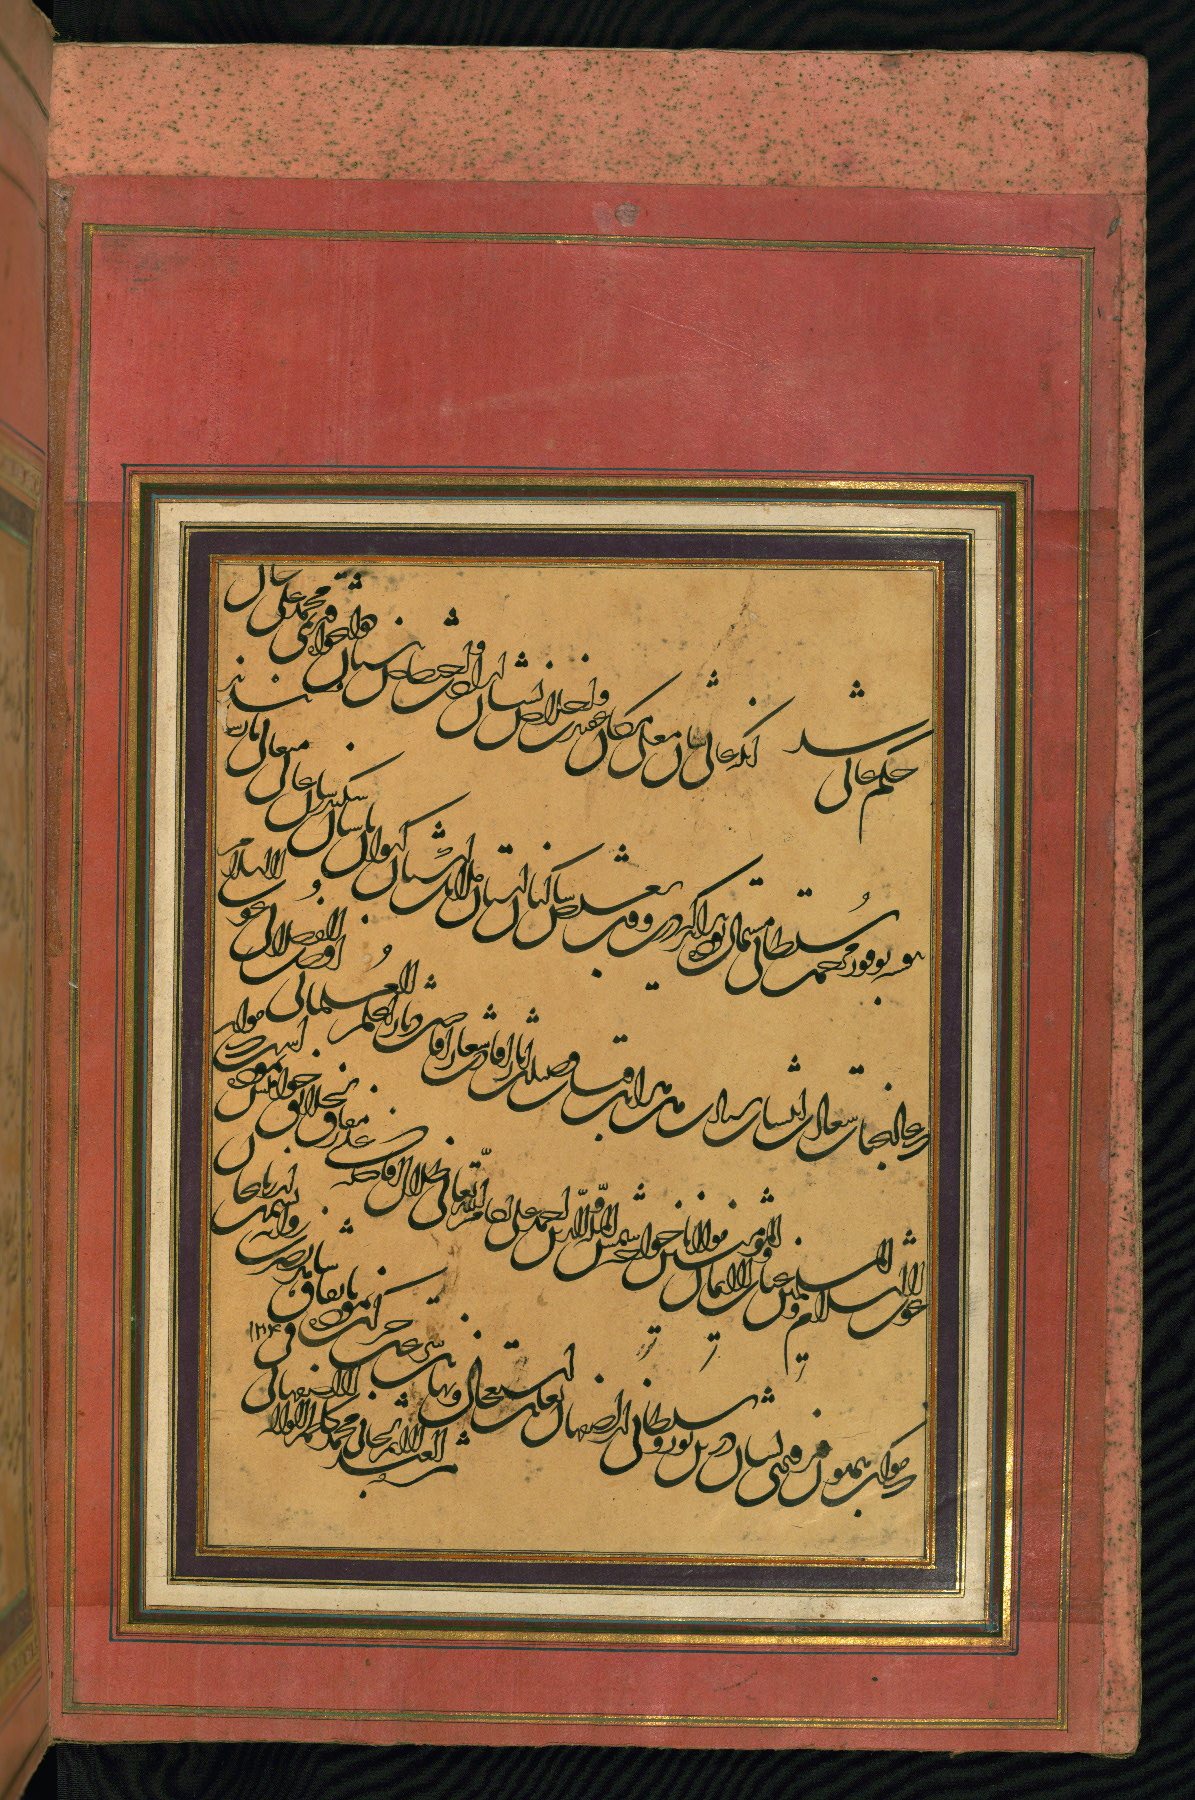
\includegraphics[width=\textwidth]{images/W670_000040_sap.jpg}
		\caption{Page from a Persian nineteenth century CE album of calligraphic samples written in \emph{taʼlīq} (Walters W.670, fol. 19b)}
                \label{fig:ara_taliq}
        \end{subfigure}
	\hfill
	\begin{subfigure}[t]{.48\columnwidth}
                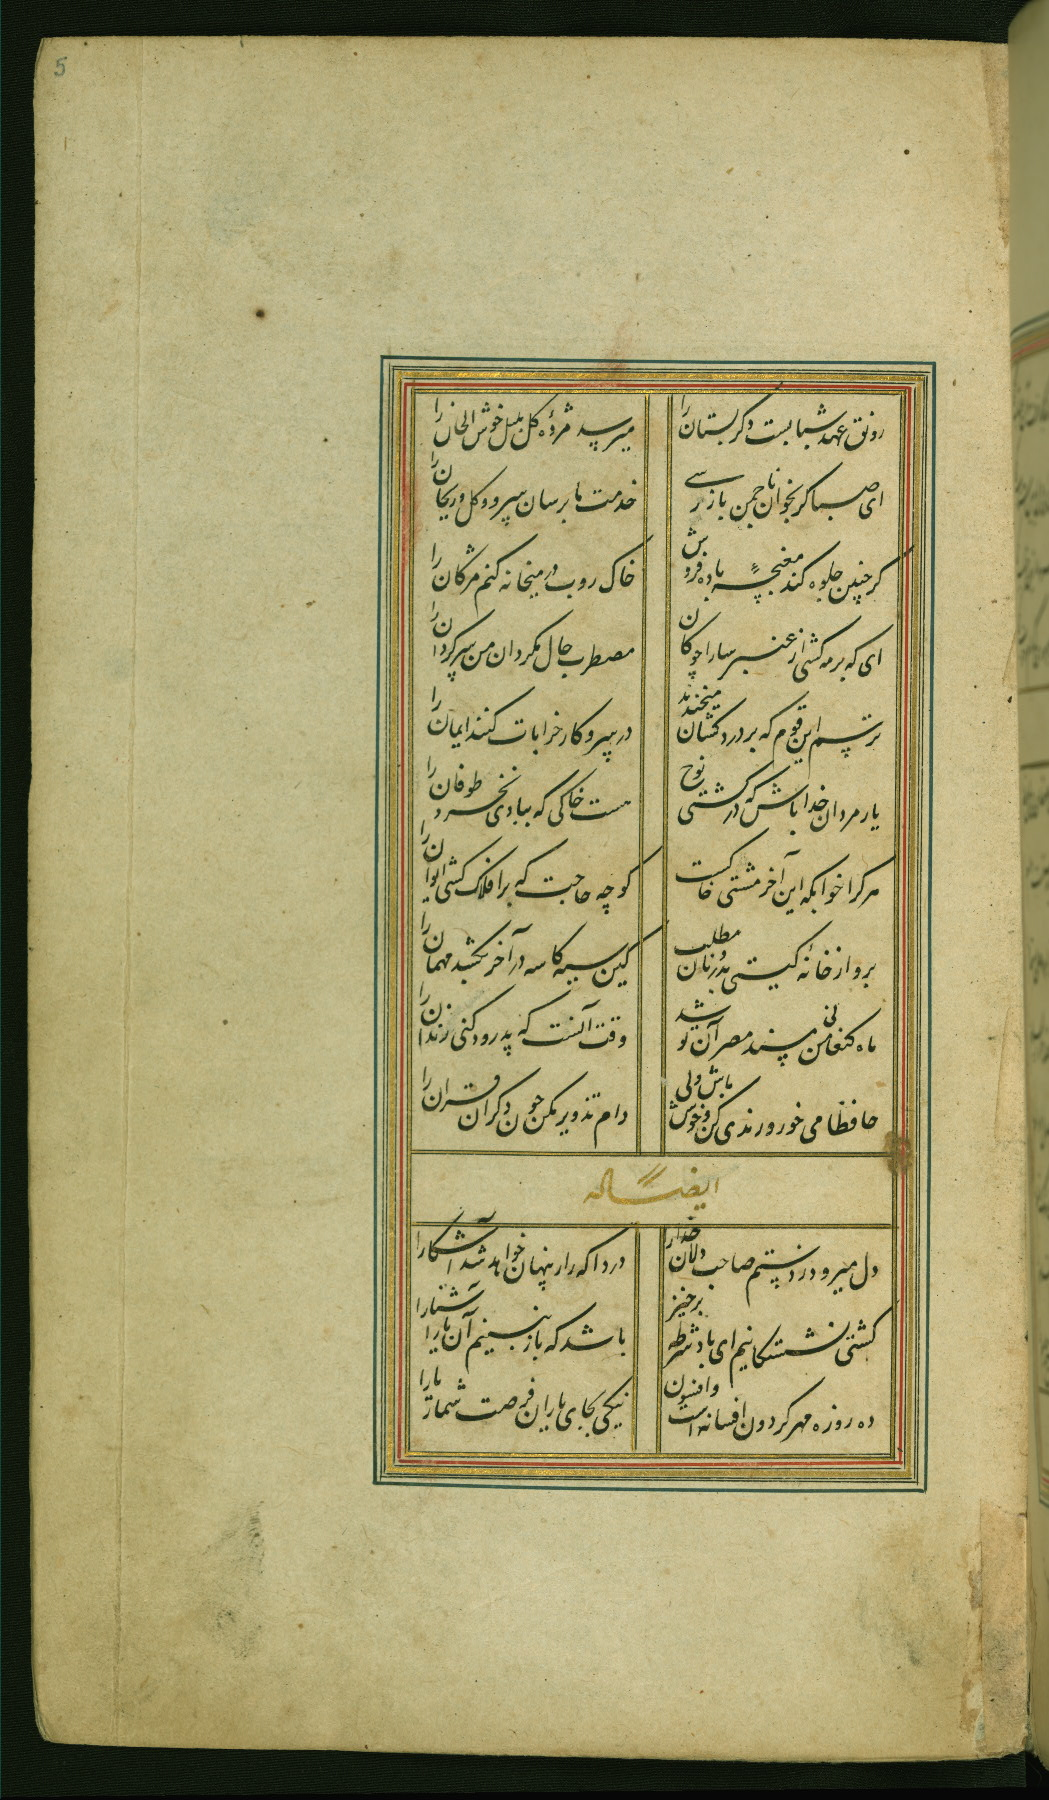
\includegraphics[width=\textwidth]{images/W631_000014_sap.jpg}
		\caption{1539 CE page from a collection of poems written in \emph{nastaʼlīq} (Walters W.631, fol. 5a)}
                \label{fig:ara_nastaliq}
        \end{subfigure}
        \vskip\baselineskip
	\begin{subfigure}[t]{.48\textwidth}
		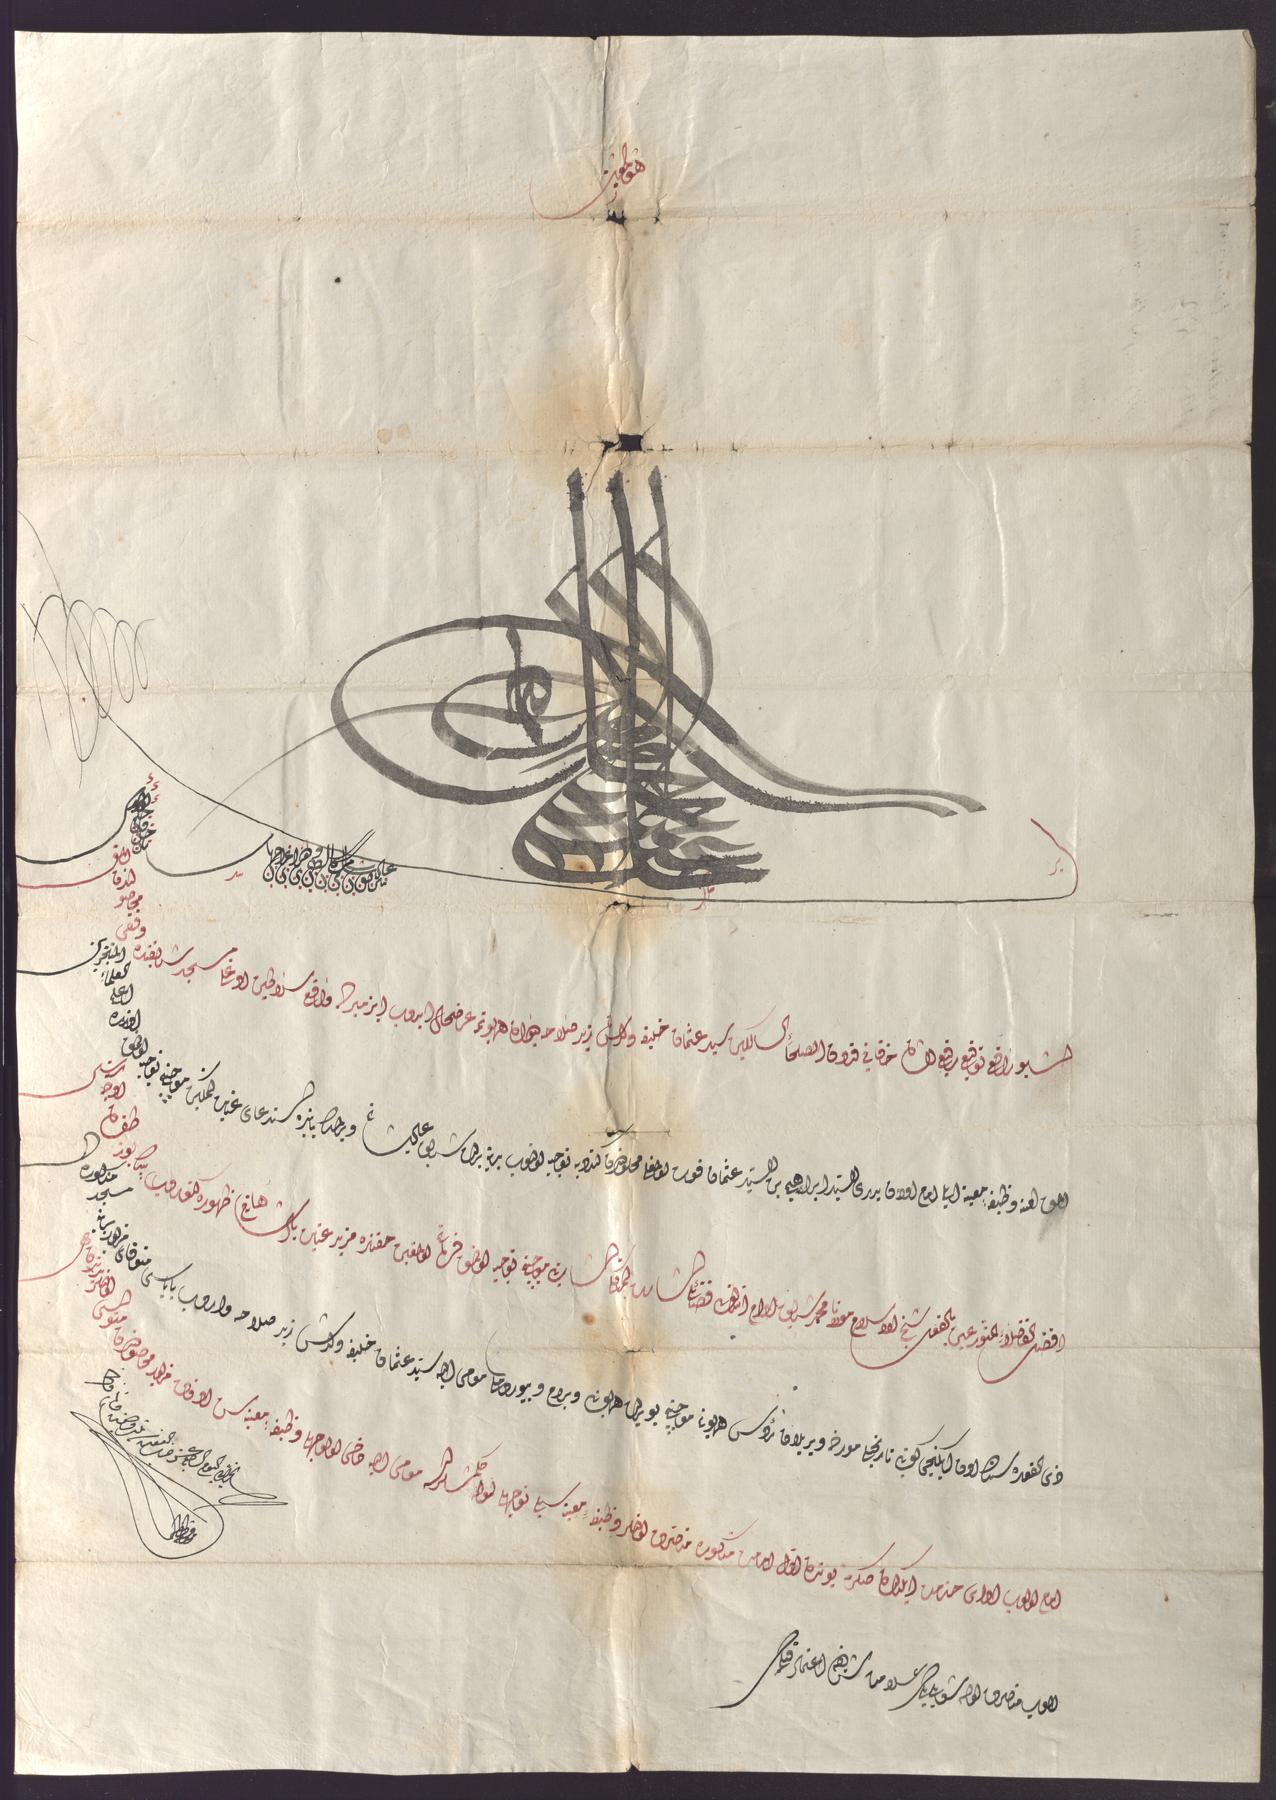
\includegraphics[width=\textwidth]{images/9676_0002_web.jpg}
		\caption{1779 CE Ottoman firman \emph{diwānī} script (American Philosophical Society Ms. Coll. 200, fol. 2)}
                \label{fig:ara_diwani}
        \end{subfigure}
	\hfill
	\begin{subfigure}[t]{.48\textwidth}
                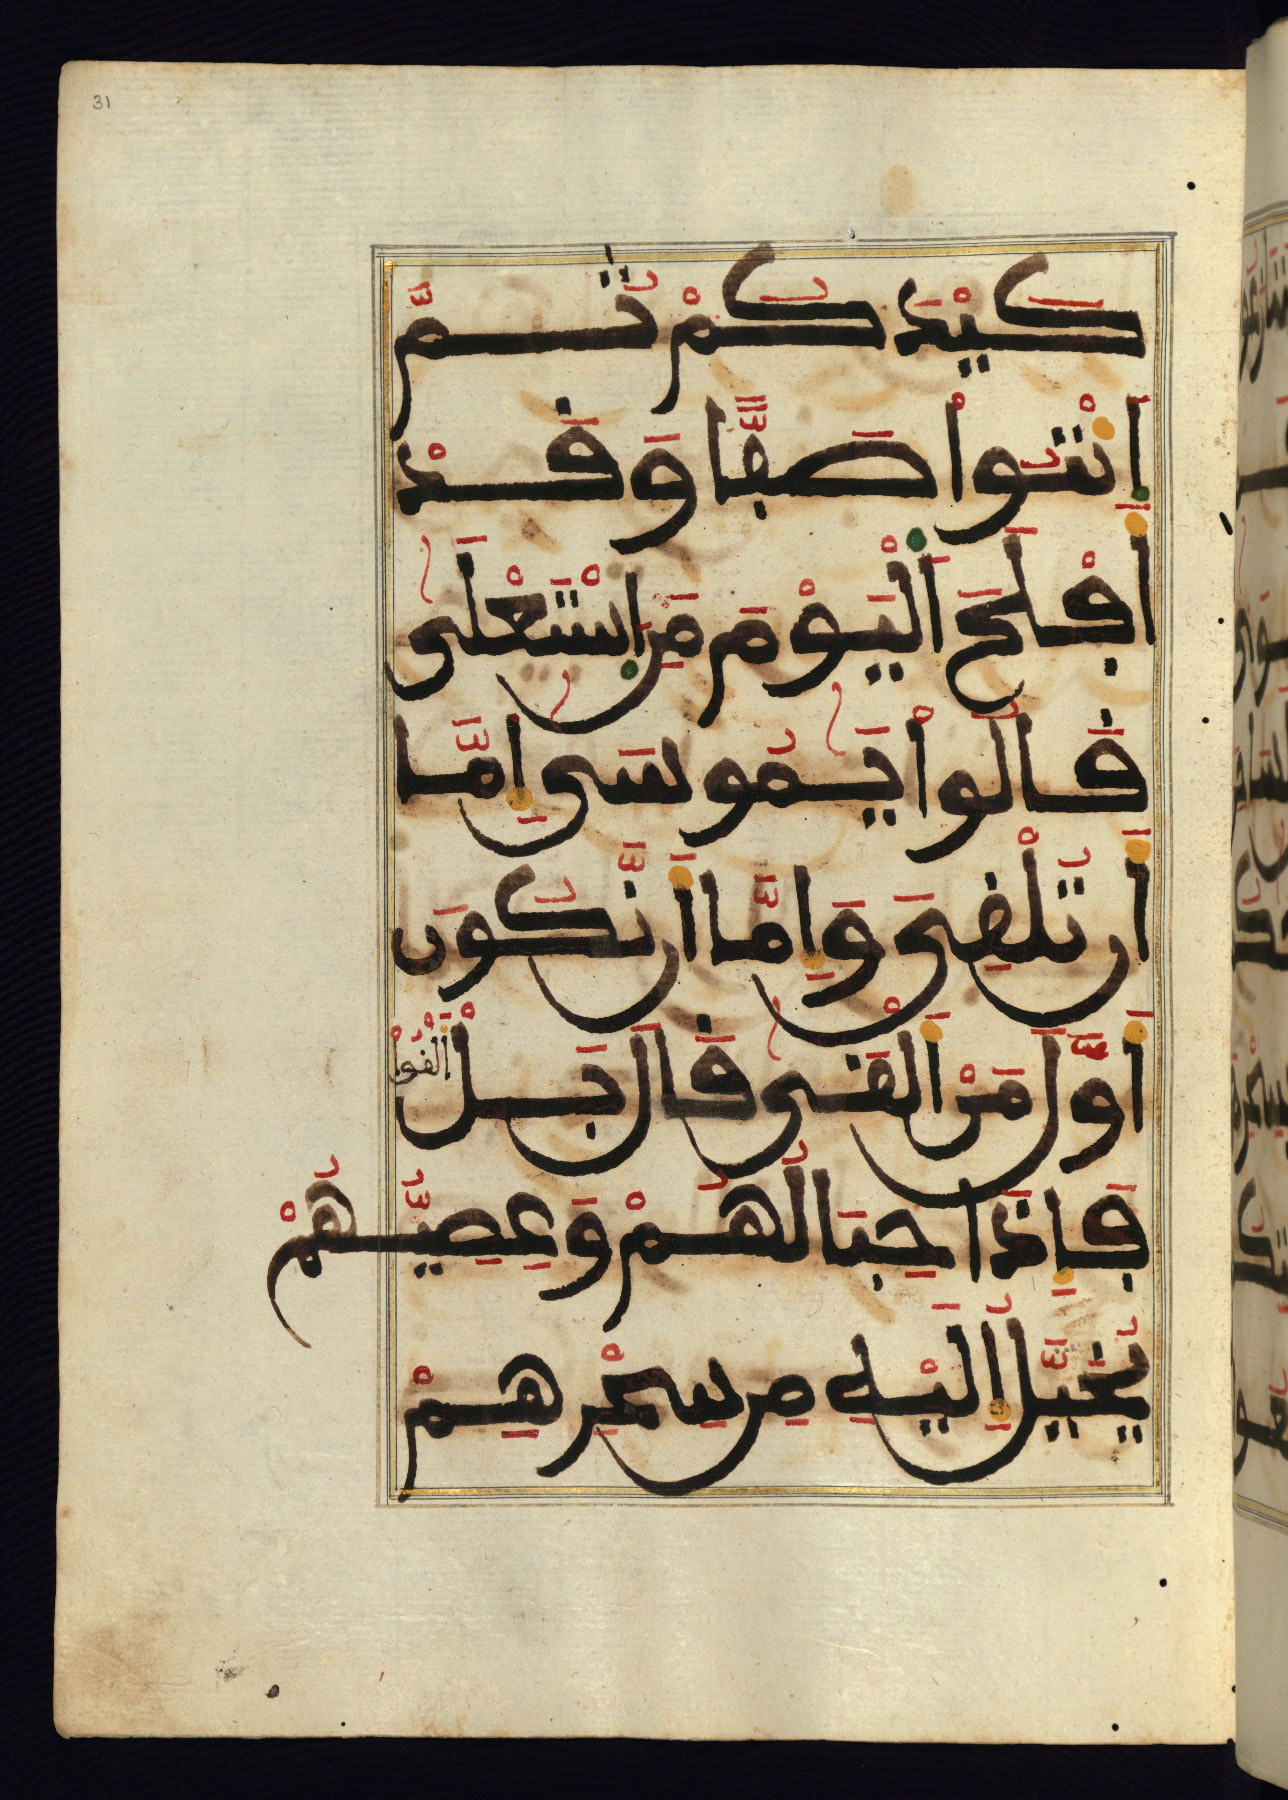
\includegraphics[width=\textwidth]{images/W568_000064_sap.jpg}
		\caption{Nineteenth century CE \emph{qurʼān} in large \emph{maghribī} script (Walters W.568, fol. 31a)}
                \label{fig:ara_maghribi}
        \end{subfigure}
        \caption{Example of regional styles}
\end{figure}


The second major Persian style, \emph{nastaʼlīq}, became the epitome of Persian
literature. At first reserved for poetry, it took over the place of
\emph{naskh} for prose by the fifteenth century as well. It is characterized by
individual words descending onto a common baseline, greatly elongated
horizontal lines, and the aforementioned heaping of the last stroke~\cite[pg.
166-167]{gacek2009arabic}. While the aforementioned styles, depending on the
preservation of the document, the desired generalization, and accuracy, are not
inherently troublesome for a modern OCR engine, the sophistication displayed by
the most decorated \emph{nastaʼlīq} epics and calligraphic specimens are highly
challenging. Calligraphers of the time were interested in variety and visual
excitement, arranging verses on the diagonal, changing direction between
successive verses, alternating red, blue, orange, and green inks for headings,
and adding lavish illumination and scrollwork. The writing was being subsumed
by decoration~\cite[pg. 436]{blair2006islamic}. 

Both round scripts, primarily \emph{naskh} and \emph{thuluth}, and Persian
hanging scripts were common in the Ottoman Empire with their relative
proportion in text production varying over the centuries\footnote{\cite[chapter
XI]{blair2006islamic} elaborates the cycles of popularity between round and
hanging scripts.} In the fifteenth century CE imperial scribes began to develop
the \emph{taʿlīq} script into the highly stylized \emph{diwānī}
(figure~\ref{fig:ara_diwani}) chancery style with its unauthorized connections
between letters and curved baselines.

\section{Printing}

While the main focus of this dissertation is the question of handwritten text
recognition, printing of the Arabic script deserves some consideration,
especially as its development and diffusion is directly linked to the practice
of calligraphy. Printing is the mechanical reproduction of text and images.
Since the printing system developed by Johannes Gutenberg around 1450 the term
has been near-synonymous with movable type printing where reverse images of
each grapheme including punctuation marks and decorations are cast in metal as
individual elements, the type. Types are arranged to form larger units, most
often whole lines, which are subsequently assembled into a matrix for a whole
page. The matrix is placed in a printing press, inked, brought into contact
with the material to be printed, usually paper, and the process is repeated as
desired. Nevertheless other kinds of printing, such as Egyptian and
Mesopotamian cylinder seals or Chinese woodblock printing, have existed for
thousands of years before Gutenberg's invention. 

In contrast to movable type printing, block printing employs a unitary matrix
carved out of a single piece of wood. The production of block printed texts has
been attested throughout Islamic world since at least 900 CE, although the
practice seems to have died out by 1430. The actual extent of the use of this
technique and its exact origins are still unknown and the low number of
block-printed documents in archives and the lack of archeological evidence for
matrices and printing equipment leave the topic mostly shrouded in obscurity.
The only preserved documents with any frequency are amulets and charms
containing quranic passages printed on paper in a wide array of styles,
generally following equivalent calligraphic practices of their handwritten
counterparts\footnote{A survey of the current state of scholarship is found in
\cite{schaefer2006enigmatic}}. As these documents have largely escaped the
scholarly interest, there are up to now no specific methods developed by the
DIA community to treat them.

Movable type printing arrived in the Islamic world at the end of the fifteenth
century CE with printing presses being set up in Constantinople and other
cities of the Ottoman Empire. While these were operating in Islamic lands, they
were run by the Jewish minority and did not produce books in Arabic script.
Evidence for the popularly held notion that the Ottoman Sultan Bayezid II
prohibited movable type printing outright, restricted it to certain scripts, or
minorities of the empire in 1485 CE is contradictory and slim
\cite{schwartz2017did} but in any case printing of the Arabic script in the
Islamic world was first performed in the workshop established by imperial
printer Ibrahim Muteferrika in 1727 CE. This does not mean that no Arabic books
were printed at all but these were exclusively imports, mostly from workshops
in Italy. The earliest preserved print is a book of hours from 1513 CE printed
in Venice by Gregorio de Gregori~\cite{krek1979enigma}. The earliest printed
edition of the \emph{qurʼān} was produced by the brother Paganino and Alessandro
Paganini in 1537-1538 CE and was an utter commercial failure as the typeface
was odd and the text itself riddled with numberous errors~\cite[pg.
219-220]{bloompaper}. Even typefaces later cut by famed type-founders such as
Robert Granjon (1585), William Caslon (1720), Giambattista Bodoni (1759) were
simplistic and of low quality~\cite{tracy1975advances}. 

Although universally derided for their lack of grace, legibility, and
orthographical correctness later imports seem to have found more popular
acceptance as lamented by Muteferrika in a 1727 CE work on the usefulness of
printing. The secular nature of the vast majority of these imports support the
theory that religious sentiment was a principal factor hindering the adoption
of printing, although the economic interests of a substantial class of scribes
and calligraphers certainly played a role, in addition to the inherent
difficulties of creating adequate typefaces for a cursive script~\cite[pg.
605]{blair2006islamic}.

Despite this multi-faceted resistance to movable type printing, some refinement
took place. While typeface cut in the Christian world were largely modelled on
the \emph{maghrebi} style, Muteferrika introduced the more legible \emph{naskh}
style in printing which remains to this day the most popular style for printed
Arabic texts. However, creating a full Arabic font remained a truly staggering
task; the Imprimerie Nationale's twenty-four-point nineteenth century CE Arabic
typeface contained 710 different types~\cite[pg. 218]{bloompaper}. In addition,
actually setting such large typefaces required skill incomparable to the much
simpler Latin script. It has been argued that apart from social objections, the
sheer laboriousness combined with a lacking industrial base made movable type
printing uneconomical in the Islamic world \cite{auji2017neither}. Indeed, the
rise of printing presses in the nineteenth century coincides with the invention
of lithography which allowed inexpensive, accurate reproductions of handwritten
texts, missionary activity and modernization drives less subject to immediate
economic pressures \cite{turner1996dictionary}. Printers like Faris al Shidyaq,
founder of the al-Jawa'ib press in Istanbul, introduced Western-style layouts
with punctuation marks and paragraphs but were not able to resolve the
laborious typesetting process or aesthetic issues such as lacking overlap of
letters, line justification limited to baseline stroke elongation instead of
the more aesthetically pleasing letter elongation or stacking, and visible gaps
between individual types~\cite[pg. 605]{blair2006islamic}. The invention of hot
type line casting machines such as the 1911 Arabic Linotype eliminated gaps
between glyphs but the limits of the machine did not allow proper placement of
vowel marks~\cite[pg. 67]{nemeth2017arabic} and subsequent iterations
economised more and more glyph variants reducing the visual appeal of the final
product. Only the advent of software-driven phototypesetters in the
nineteen-sixties make sufficiently large type repertoires including contextual
and elongated forms economically feasable. Even though the last vestiges of the
limitations of physical type have disappeared with purely digital typesetters,
most common typefacess do not make use of these.

A closer study on the limitations of current OCR technology on modern printed
Arabic texts follows in the next chapter.

\section{Basic requirements for Arabic OCR systems}

In summary the recognition of Arabic handwritten texts requires a number of
design decisions and features not commonly found in available OCR engines. Not
all of them have been addressed as part of this dissertation, chiefly because
of a lack of available Arabic-script or substitute training data. The principal
ones are, in order of processing inside a typical pipeline:

\begin{description}
	\item[Freedom of Binarization] The variety of supports employed in
		writing Arabic, the often fragmentary nature of writing on
		Papyrus, faded and acid-damaged writing in iron-gall inks, and
		highly decorated pages make it impossible to devise a general
		binarization method applicable to most Arabic handwriting.
		While trainable methods using semantic segmentation approaches
		exist, their training data requirements are frequently
		insurmountable.
	\item[Segmentation of curved and slanted lines] The frequent use of
		baseline curvature and slanted lines for both practical and
		aesthetic purposes requires a layout analysis (LA) method
		capable of modelling lines in a way that allows normalization
		of the axis of writing and the effective suppression of
		non-line content.
	\item[Semantic layout analysis] Many Arabic manuscripts contain an
		unusual amount of paratext or textual \emph{noise}, be it
		marginal notes, parallel texts, interlinear translations, or
		detached word fragments. Proper treatment of these elements,
		e.g. separation of commentary from maint text or selection of
		the appropriate recognition model for a parallel text in
		another script, requires at least in part awareness of these
		elements in the LA component. As the types of elements, their
		presentation, and frequency can vary immensely it is highly
		desirable for the LA system to be trainable.
	\item[Advanced reading order determination] Related to the
		classification of textual components in the LA module is the
		correct ordering of the texts and the proper linking of
		paratextual components to the main text. As mentioned before
		this is a nacent field of research and all OCR systems
		available infer the order of text using highly flawed
		heuristics.
	\item[Segmentation-free transcription] The cursive nature of Arabic
		writing, particularly the variation of letter connections
		encountered between different scripts makes reliable
		segmentation into single graphemes impractical for handwritten
		texts, especially so when executed in highly stylized and
		contracted scripts. While a significant body of literature
		exist on this problem, the success of sequence-to-sequence
		machine learning models, that require no or only implicit
		segmentation/alignment of input image data and characters, have
		rendered the problem largely moot.
	\item[Data creation and curation tools] While not a direct part of an
		OCR pipeline, especially one employed in large-scale archival
		or library digitization pro\-jects, the lack of open tools
		adapted to create training data that can capture the pertinent
		features of Arabic handwritten text and the subsequent lack of
		training data sets available for DIA research has stifled the
		field. Simple transcription tools such as the one utilized for
		the study in chapter~\ref{ch:champs} are inadequate for
		preparing multi-purpose datasets. Fully featured Virtual
		Research Environments (VREs) for palaeographic scholarly work
		are one way to attain deeply annotated data in flexible
		non-writing-system-specific data models.
\end{description}

In addition there are minor technical requirements that do not present a true
research question but are sometimes disregarded. The most glaring one often
missing from older or purely research software is support for non-ASCII and
bidirectional text requiring manual substitution and reordering of code points.
More subtle sources of errors such as overly aggressive normalization of input
text, lack of Unicode white space normalization, and the treatment of
non-printing code points are also prevalent and often difficult to ascertain,
especially in proprietary software. 

It should be noted that while the underlying reasons for implementing these
requirements are specific to the Arabic script, comparable features exist in
documents written in other scripts. The motivations for binarization-freedom
are applicable to more or less any historical written document; the same
applies to curved handwriting, marginalia, and parallel texts. Tailoring an OCR
system to better process Arabic texts therefore \emph{enhances} the capability
to process most other texts as well.

\phantomsection
\printbibliography[heading=subbibliography]
\endrefsection

\printbibliography[heading=subbibliography]
\end{refsection}
\begin{refsection}
\import{./chapters/champs}{advances.tex}
\printbibliography[heading=subbibliography]
\end{refsection}
\part{Layout Analysis and Segmentation}
\begin{refsection}
\import{./chapters/hip}{icdar}
\printbibliography[heading=subbibliography]
\end{refsection}
\begin{refsection}
\import{./chapters/icfhr2020}{seg}
\printbibliography[heading=subbibliography]
\end{refsection}
\cleardoublepage
%\begin{refsection}
%\import{./chapters/read}{read}
%\printbibliography[heading=subbibliography]
%\end{refsection}

\part{Transcription and Character Alignment}
\cleardoublepage
\begin{refsection}
\import{./chapters/dh2019}{dh}
\printbibliography[heading=subbibliography]
\end{refsection}
\begin{refsection}
\import{./chapters/icfhr2020algn}{Transcribe}
\printbibliography[heading=subbibliography]
\end{refsection}

\part{The Escriptorium VRE}
\cleardoublepage
\begin{refsection}
\import{./chapters/manuvre}{vre}
\printbibliography[heading=subbibliography]
\end{refsection}

\appendix

\label{annex:vgsl}


\printbibliography

\end{document}
